% This is samplepaper.tex, a sample chapter demonstrating the
% LLNCS macro package for Springer Computer Science proceedings;
% Version 2.21 of 2022/01/12
%
\documentclass[runningheads]{llncs}
%
\usepackage[T1]{fontenc}
% T1 fonts will be used to generate the final print and online PDFs,
% so please use T1 fonts in your manuscript whenever possible.
% Other font encondings may result in incorrect characters.
%
\usepackage{graphicx}
% Used for displaying a sample figure. If possible, figure files should
% be included in EPS format.
\usepackage{latexsym}
\usepackage{algorithm}
\usepackage[noend]{algorithmic}
\usepackage{amssymb}
\usepackage{amsmath}
% \usepackage{amsthm}
\usepackage{booktabs}
\usepackage[inline]{enumitem}
\usepackage{graphicx}
\usepackage{hyperref}
\usepackage{environ}
\usepackage{marginnote}
\usepackage{multirow}
% \usepackage[numbers]{natbib}
% \usepackage{paralist}
\usepackage{pgfplots}
\usepackage{pifont}
\usepackage{placeins}
\usepackage{rotate} 
\usepackage[draft]{todonotes}
%\usepackage[disable]{todonotes}
\usepackage{tikz}
\usepackage{times} 
\usepackage{url}
\usepackage{varwidth}
\usepackage{verbatim} 
\usepackage{wrapfig}
\usepackage{xcolor,colortbl}
\usepackage{xspace}
\usepackage{subcaption}
\usepackage{tabularx}
\usetikzlibrary{intersections, backgrounds, calc}
\usepackage{cleveref}
%
% If you use the hyperref package, please uncomment the following two lines
% to display URLs in blue roman font according to Springer's eBook style:
\usepackage{color}
\renewcommand\UrlFont{\color{blue}\rmfamily}
\urlstyle{rm}

\renewcommand{\topfraction}{.8}
\renewcommand{\floatpagefraction}{.8}

%
\begin{document}

%%%%%%%%%%%%%%%%%%%%%%%%%%%%%%%%%%%%%%%%%%%%%%%%%%%%%%%%%%%%%%%%%%%%
%%%%%%% This file is an hard link, whose source is in   
%%%%%%% cipeciop.science.unitn.it:/home/rseba/latex/macros
%%%%%%%%%%%%%%%%%%%%%%%%%%%%%%%%%%%%%%%%%%%%%%%%%%%%%%%%%%%%%%%%%%%%

%%%%%%%%%%%%%%%%%%%%%%%%%%%%%%%%%%%%%%%%%%%%%%%%%%%%%%%%%%%%%
%%% general-use macros 
%%%%%%%%%%%%%%%%%%%%%%%%%%%%%%%%%%%%%%%%%%%%%%%%%%%%%%%%%%%%%

%% rgb.tex
%% this file defines the X11 rgb color names for use with pstricks
%% put \usepackage{pstricks, pstcol} in the preamble of your document
%% the put 
%% rgb.tex
%% this file defines the X11 rgb color names for use with pstricks
%% put \usepackage{pstricks, pstcol} in the preamble of your document
%% the put \input{rgb.tex} in the body of your document.
%% Color in pstricks works like a switch.  If you enter
%%    The text will become \color{red}red.
%% Then all text after the \color command will printed in red in the
%% postscript file.  You can restrict the range of the red text in this
%% manner
%%    One {\color{red}some text} will be red.
%% The color will NOT show up in the dvi file, only in the .ps file!
%%
%% this file was created by rgb2tex.pl
%% rgb2tex.pl is by Bruce Ravel <bruce.ravel@nist.gov>
%% --------------------------------------------------------------------------

\definecolor{snow}                {rgb}{1.00,0.98,0.98}
\definecolor{ghostwhite}          {rgb}{0.97,0.97,1.00}
\definecolor{whitesmoke}          {rgb}{0.96,0.96,0.96}
\definecolor{gainsboro}           {rgb}{0.86,0.86,0.86}
\definecolor{floralwhite}         {rgb}{1.00,0.98,0.94}
\definecolor{oldlace}             {rgb}{0.99,0.96,0.90}
\definecolor{linen}               {rgb}{0.98,0.94,0.90}
\definecolor{antiquewhite}        {rgb}{0.98,0.92,0.84}
\definecolor{papayawhip}          {rgb}{1.00,0.94,0.84}
\definecolor{blanchedalmond}      {rgb}{1.00,0.92,0.80}
\definecolor{bisque}              {rgb}{1.00,0.89,0.77}
\definecolor{peachpuff}           {rgb}{1.00,0.85,0.73}
\definecolor{navajowhite}         {rgb}{1.00,0.87,0.68}
\definecolor{moccasin}            {rgb}{1.00,0.89,0.71}
\definecolor{cornsilk}            {rgb}{1.00,0.97,0.86}
\definecolor{ivory}               {rgb}{1.00,1.00,0.94}
\definecolor{lemonchiffon}        {rgb}{1.00,0.98,0.80}
\definecolor{seashell}            {rgb}{1.00,0.96,0.93}
\definecolor{honeydew}            {rgb}{0.94,1.00,0.94}
\definecolor{mintcream}           {rgb}{0.96,1.00,0.98}
\definecolor{azure}               {rgb}{0.94,1.00,1.00}
\definecolor{aliceblue}           {rgb}{0.94,0.97,1.00}
\definecolor{lavender}            {rgb}{0.90,0.90,0.98}
\definecolor{lavenderblush}       {rgb}{1.00,0.94,0.96}
\definecolor{mistyrose}           {rgb}{1.00,0.89,0.88}
\definecolor{white}               {rgb}{1.00,1.00,1.00}
\definecolor{black}               {rgb}{0.00,0.00,0.00}
\definecolor{darkslategray}       {rgb}{0.18,0.31,0.31}
\definecolor{dimgray}             {rgb}{0.41,0.41,0.41}
\definecolor{slategray}           {rgb}{0.44,0.50,0.56}
\definecolor{lightslategray}      {rgb}{0.47,0.53,0.60}
\definecolor{gray}                {rgb}{0.75,0.75,0.75}
\definecolor{lightgrey}           {rgb}{0.83,0.83,0.83}
\definecolor{midnightblue}        {rgb}{0.10,0.10,0.44}
\definecolor{navy}                {rgb}{0.00,0.00,0.50}
\definecolor{cornflowerblue}      {rgb}{0.39,0.58,0.93}
\definecolor{darkslateblue}       {rgb}{0.28,0.24,0.55}
\definecolor{slateblue}           {rgb}{0.42,0.35,0.80}
\definecolor{mediumslateblue}     {rgb}{0.48,0.41,0.93}
\definecolor{lightslateblue}      {rgb}{0.52,0.44,1.00}
\definecolor{mediumblue}          {rgb}{0.00,0.00,0.80}
\definecolor{royalblue}           {rgb}{0.25,0.41,0.88}
\definecolor{blue}                {rgb}{0.00,0.00,1.00}
\definecolor{dodgerblue}          {rgb}{0.12,0.56,1.00}
\definecolor{deepskyblue}         {rgb}{0.00,0.75,1.00}
\definecolor{skyblue}             {rgb}{0.53,0.81,0.92}
\definecolor{lightskyblue}        {rgb}{0.53,0.81,0.98}
\definecolor{steelblue}           {rgb}{0.27,0.51,0.71}
\definecolor{lightsteelblue}      {rgb}{0.69,0.77,0.87}
\definecolor{lightblue}           {rgb}{0.68,0.85,0.90}
\definecolor{powderblue}          {rgb}{0.69,0.88,0.90}
\definecolor{paleturquoise}       {rgb}{0.69,0.93,0.93}
\definecolor{darkturquoise}       {rgb}{0.00,0.81,0.82}
\definecolor{mediumturquoise}     {rgb}{0.28,0.82,0.80}
\definecolor{turquoise}           {rgb}{0.25,0.88,0.82}
\definecolor{cyan}                {rgb}{0.00,1.00,1.00}
\definecolor{lightcyan}           {rgb}{0.88,1.00,1.00}
\definecolor{cadetblue}           {rgb}{0.37,0.62,0.63}
\definecolor{mediumaquamarine}    {rgb}{0.40,0.80,0.67}
\definecolor{aquamarine}          {rgb}{0.50,1.00,0.83}
\definecolor{darkgreen}           {rgb}{0.00,0.39,0.00}
\definecolor{darkolivegreen}      {rgb}{0.33,0.42,0.18}
\definecolor{darkseagreen}        {rgb}{0.56,0.74,0.56}
\definecolor{seagreen}            {rgb}{0.18,0.55,0.34}
\definecolor{mediumseagreen}      {rgb}{0.24,0.70,0.44}
\definecolor{lightseagreen}       {rgb}{0.13,0.70,0.67}
\definecolor{palegreen}           {rgb}{0.60,0.98,0.60}
\definecolor{springgreen}         {rgb}{0.00,1.00,0.50}
\definecolor{lawngreen}           {rgb}{0.49,0.99,0.00}
\definecolor{green}               {rgb}{0.00,1.00,0.00}
\definecolor{chartreuse}          {rgb}{0.50,1.00,0.00}
\definecolor{mediumspringgreen}   {rgb}{0.00,0.98,0.60}
\definecolor{greenyellow}         {rgb}{0.68,1.00,0.18}
\definecolor{limegreen}           {rgb}{0.20,0.80,0.20}
\definecolor{yellowgreen}         {rgb}{0.60,0.80,0.20}
\definecolor{forestgreen}         {rgb}{0.13,0.55,0.13}
\definecolor{olivedrab}           {rgb}{0.42,0.56,0.14}
\definecolor{darkkhaki}           {rgb}{0.74,0.72,0.42}
\definecolor{khaki}               {rgb}{0.94,0.90,0.55}
\definecolor{palegoldenrod}       {rgb}{0.93,0.91,0.67}
\definecolor{lightgoldenrodyellow} {rgb}{0.98,0.98,0.82}
\definecolor{lightyellow}         {rgb}{1.00,1.00,0.88}
\definecolor{yellow}              {rgb}{1.00,1.00,0.00}
\definecolor{gold}                {rgb}{1.00,0.84,0.00}
\definecolor{lightgoldenrod}      {rgb}{0.93,0.87,0.51}
\definecolor{goldenrod}           {rgb}{0.85,0.65,0.13}
\definecolor{darkgoldenrod}       {rgb}{0.72,0.53,0.04}
\definecolor{rosybrown}           {rgb}{0.74,0.56,0.56}
\definecolor{indianred}           {rgb}{0.80,0.36,0.36}
\definecolor{saddlebrown}         {rgb}{0.55,0.27,0.07}
\definecolor{sienna}              {rgb}{0.63,0.32,0.18}
\definecolor{peru}                {rgb}{0.80,0.52,0.25}
\definecolor{burlywood}           {rgb}{0.87,0.72,0.53}
\definecolor{beige}               {rgb}{0.96,0.96,0.86}
\definecolor{wheat}               {rgb}{0.96,0.87,0.70}
\definecolor{sandybrown}          {rgb}{0.96,0.64,0.38}
\definecolor{tan}                 {rgb}{0.82,0.71,0.55}
\definecolor{chocolate}           {rgb}{0.82,0.41,0.12}
\definecolor{firebrick}           {rgb}{0.70,0.13,0.13}
\definecolor{brown}               {rgb}{0.65,0.16,0.16}
\definecolor{darksalmon}          {rgb}{0.91,0.59,0.48}
\definecolor{salmon}              {rgb}{0.98,0.50,0.45}
\definecolor{lightsalmon}         {rgb}{1.00,0.63,0.48}
\definecolor{orange}              {rgb}{1.00,0.65,0.00}
\definecolor{darkorange}          {rgb}{1.00,0.55,0.00}
\definecolor{coral}               {rgb}{1.00,0.50,0.31}
\definecolor{lightcoral}          {rgb}{0.94,0.50,0.50}
\definecolor{tomato}              {rgb}{1.00,0.39,0.28}
\definecolor{orangered}           {rgb}{1.00,0.27,0.00}
\definecolor{red}                 {rgb}{1.00,0.00,0.00}
\definecolor{hotpink}             {rgb}{1.00,0.41,0.71}
\definecolor{deeppink}            {rgb}{1.00,0.08,0.58}
\definecolor{pink}                {rgb}{1.00,0.75,0.80}
\definecolor{lightpink}           {rgb}{1.00,0.71,0.76}
\definecolor{palevioletred}       {rgb}{0.86,0.44,0.58}
\definecolor{maroon}              {rgb}{0.69,0.19,0.38}
\definecolor{mediumvioletred}     {rgb}{0.78,0.08,0.52}
\definecolor{violetred}           {rgb}{0.82,0.13,0.56}
\definecolor{magenta}             {rgb}{1.00,0.00,1.00}
\definecolor{violet}              {rgb}{0.93,0.51,0.93}
\definecolor{plum}                {rgb}{0.87,0.63,0.87}
\definecolor{orchid}              {rgb}{0.85,0.44,0.84}
\definecolor{mediumorchid}        {rgb}{0.73,0.33,0.83}
\definecolor{darkorchid}          {rgb}{0.60,0.20,0.80}
\definecolor{darkviolet}          {rgb}{0.58,0.00,0.83}
\definecolor{blueviolet}          {rgb}{0.54,0.17,0.89}
\definecolor{purple}              {rgb}{0.63,0.13,0.94}
\definecolor{mediumpurple}        {rgb}{0.58,0.44,0.86}
\definecolor{thistle}             {rgb}{0.85,0.75,0.85}
\definecolor{snow2}               {rgb}{0.93,0.91,0.91}
\definecolor{snow3}               {rgb}{0.80,0.79,0.79}
\definecolor{snow4}               {rgb}{0.55,0.54,0.54}
\definecolor{seashell2}           {rgb}{0.93,0.90,0.87}
\definecolor{seashell3}           {rgb}{0.80,0.77,0.75}
\definecolor{seashell4}           {rgb}{0.55,0.53,0.51}
\definecolor{antiquewhite1}       {rgb}{1.00,0.94,0.86}
\definecolor{antiquewhite2}       {rgb}{0.93,0.87,0.80}
\definecolor{antiquewhite3}       {rgb}{0.80,0.75,0.69}
\definecolor{antiquewhite4}       {rgb}{0.55,0.51,0.47}
\definecolor{bisque2}             {rgb}{0.93,0.84,0.72}
\definecolor{bisque3}             {rgb}{0.80,0.72,0.62}
\definecolor{bisque4}             {rgb}{0.55,0.49,0.42}
\definecolor{peachpuff2}          {rgb}{0.93,0.80,0.68}
\definecolor{peachpuff3}          {rgb}{0.80,0.69,0.58}
\definecolor{peachpuff4}          {rgb}{0.55,0.47,0.40}
\definecolor{navajowhite2}        {rgb}{0.93,0.81,0.63}
\definecolor{navajowhite3}        {rgb}{0.80,0.70,0.55}
\definecolor{navajowhite4}        {rgb}{0.55,0.47,0.37}
\definecolor{lemonchiffon2}       {rgb}{0.93,0.91,0.75}
\definecolor{lemonchiffon3}       {rgb}{0.80,0.79,0.65}
\definecolor{lemonchiffon4}       {rgb}{0.55,0.54,0.44}
\definecolor{cornsilk2}           {rgb}{0.93,0.91,0.80}
\definecolor{cornsilk3}           {rgb}{0.80,0.78,0.69}
\definecolor{cornsilk4}           {rgb}{0.55,0.53,0.47}
\definecolor{ivory2}              {rgb}{0.93,0.93,0.88}
\definecolor{ivory3}              {rgb}{0.80,0.80,0.76}
\definecolor{ivory4}              {rgb}{0.55,0.55,0.51}
\definecolor{honeydew2}           {rgb}{0.88,0.93,0.88}
\definecolor{honeydew3}           {rgb}{0.76,0.80,0.76}
\definecolor{honeydew4}           {rgb}{0.51,0.55,0.51}
\definecolor{lavenderblush2}      {rgb}{0.93,0.88,0.90}
\definecolor{lavenderblush3}      {rgb}{0.80,0.76,0.77}
\definecolor{lavenderblush4}      {rgb}{0.55,0.51,0.53}
\definecolor{mistyrose2}          {rgb}{0.93,0.84,0.82}
\definecolor{mistyrose3}          {rgb}{0.80,0.72,0.71}
\definecolor{mistyrose4}          {rgb}{0.55,0.49,0.48}
\definecolor{azure2}              {rgb}{0.88,0.93,0.93}
\definecolor{azure3}              {rgb}{0.76,0.80,0.80}
\definecolor{azure4}              {rgb}{0.51,0.55,0.55}
\definecolor{slateblue1}          {rgb}{0.51,0.44,1.00}
\definecolor{slateblue2}          {rgb}{0.48,0.40,0.93}
\definecolor{slateblue3}          {rgb}{0.41,0.35,0.80}
\definecolor{slateblue4}          {rgb}{0.28,0.24,0.55}
\definecolor{royalblue1}          {rgb}{0.28,0.46,1.00}
\definecolor{royalblue2}          {rgb}{0.26,0.43,0.93}
\definecolor{royalblue3}          {rgb}{0.23,0.37,0.80}
\definecolor{royalblue4}          {rgb}{0.15,0.25,0.55}
\definecolor{blue2}               {rgb}{0.00,0.00,0.93}
\definecolor{blue4}               {rgb}{0.00,0.00,0.55}
\definecolor{dodgerblue2}         {rgb}{0.11,0.53,0.93}
\definecolor{dodgerblue3}         {rgb}{0.09,0.45,0.80}
\definecolor{dodgerblue4}         {rgb}{0.06,0.31,0.55}
\definecolor{steelblue1}          {rgb}{0.39,0.72,1.00}
\definecolor{steelblue2}          {rgb}{0.36,0.67,0.93}
\definecolor{steelblue3}          {rgb}{0.31,0.58,0.80}
\definecolor{steelblue4}          {rgb}{0.21,0.39,0.55}
\definecolor{deepskyblue2}        {rgb}{0.00,0.70,0.93}
\definecolor{deepskyblue3}        {rgb}{0.00,0.60,0.80}
\definecolor{deepskyblue4}        {rgb}{0.00,0.41,0.55}
\definecolor{skyblue1}            {rgb}{0.53,0.81,1.00}
\definecolor{skyblue2}            {rgb}{0.49,0.75,0.93}
\definecolor{skyblue3}            {rgb}{0.42,0.65,0.80}
\definecolor{skyblue4}            {rgb}{0.29,0.44,0.55}
\definecolor{lightskyblue1}       {rgb}{0.69,0.89,1.00}
\definecolor{lightskyblue2}       {rgb}{0.64,0.83,0.93}
\definecolor{lightskyblue3}       {rgb}{0.55,0.71,0.80}
\definecolor{lightskyblue4}       {rgb}{0.38,0.48,0.55}
\definecolor{slategray1}          {rgb}{0.78,0.89,1.00}
\definecolor{slategray2}          {rgb}{0.73,0.83,0.93}
\definecolor{slategray3}          {rgb}{0.62,0.71,0.80}
\definecolor{slategray4}          {rgb}{0.42,0.48,0.55}
\definecolor{lightsteelblue1}     {rgb}{0.79,0.88,1.00}
\definecolor{lightsteelblue2}     {rgb}{0.74,0.82,0.93}
\definecolor{lightsteelblue3}     {rgb}{0.64,0.71,0.80}
\definecolor{lightsteelblue4}     {rgb}{0.43,0.48,0.55}
\definecolor{lightblue1}          {rgb}{0.75,0.94,1.00}
\definecolor{lightblue2}          {rgb}{0.70,0.87,0.93}
\definecolor{lightblue3}          {rgb}{0.60,0.75,0.80}
\definecolor{lightblue4}          {rgb}{0.41,0.51,0.55}
\definecolor{lightcyan2}          {rgb}{0.82,0.93,0.93}
\definecolor{lightcyan3}          {rgb}{0.71,0.80,0.80}
\definecolor{lightcyan4}          {rgb}{0.48,0.55,0.55}
\definecolor{paleturquoise1}      {rgb}{0.73,1.00,1.00}
\definecolor{paleturquoise2}      {rgb}{0.68,0.93,0.93}
\definecolor{paleturquoise3}      {rgb}{0.59,0.80,0.80}
\definecolor{paleturquoise4}      {rgb}{0.40,0.55,0.55}
\definecolor{cadetblue1}          {rgb}{0.60,0.96,1.00}
\definecolor{cadetblue2}          {rgb}{0.56,0.90,0.93}
\definecolor{cadetblue3}          {rgb}{0.48,0.77,0.80}
\definecolor{cadetblue4}          {rgb}{0.33,0.53,0.55}
\definecolor{turquoise1}          {rgb}{0.00,0.96,1.00}
\definecolor{turquoise2}          {rgb}{0.00,0.90,0.93}
\definecolor{turquoise3}          {rgb}{0.00,0.77,0.80}
\definecolor{turquoise4}          {rgb}{0.00,0.53,0.55}
\definecolor{cyan2}               {rgb}{0.00,0.93,0.93}
\definecolor{cyan3}               {rgb}{0.00,0.80,0.80}
\definecolor{cyan4}               {rgb}{0.00,0.55,0.55}
\definecolor{darkslategray1}      {rgb}{0.59,1.00,1.00}
\definecolor{darkslategray2}      {rgb}{0.55,0.93,0.93}
\definecolor{darkslategray3}      {rgb}{0.47,0.80,0.80}
\definecolor{darkslategray4}      {rgb}{0.32,0.55,0.55}
\definecolor{aquamarine2}         {rgb}{0.46,0.93,0.78}
\definecolor{aquamarine4}         {rgb}{0.27,0.55,0.45}
\definecolor{darkseagreen1}       {rgb}{0.76,1.00,0.76}
\definecolor{darkseagreen2}       {rgb}{0.71,0.93,0.71}
\definecolor{darkseagreen3}       {rgb}{0.61,0.80,0.61}
\definecolor{darkseagreen4}       {rgb}{0.41,0.55,0.41}
\definecolor{seagreen1}           {rgb}{0.33,1.00,0.62}
\definecolor{seagreen2}           {rgb}{0.31,0.93,0.58}
\definecolor{seagreen3}           {rgb}{0.26,0.80,0.50}
\definecolor{palegreen1}          {rgb}{0.60,1.00,0.60}
\definecolor{palegreen2}          {rgb}{0.56,0.93,0.56}
\definecolor{palegreen3}          {rgb}{0.49,0.80,0.49}
\definecolor{palegreen4}          {rgb}{0.33,0.55,0.33}
\definecolor{springgreen2}        {rgb}{0.00,0.93,0.46}
\definecolor{springgreen3}        {rgb}{0.00,0.80,0.40}
\definecolor{springgreen4}        {rgb}{0.00,0.55,0.27}
\definecolor{green2}              {rgb}{0.00,0.93,0.00}
\definecolor{green3}              {rgb}{0.00,0.80,0.00}
\definecolor{green4}              {rgb}{0.00,0.55,0.00}
\definecolor{chartreuse2}         {rgb}{0.46,0.93,0.00}
\definecolor{chartreuse3}         {rgb}{0.40,0.80,0.00}
\definecolor{chartreuse4}         {rgb}{0.27,0.55,0.00}
\definecolor{olivedrab1}          {rgb}{0.75,1.00,0.24}
\definecolor{olivedrab2}          {rgb}{0.70,0.93,0.23}
\definecolor{olivedrab4}          {rgb}{0.41,0.55,0.13}
\definecolor{darkolivegreen1}     {rgb}{0.79,1.00,0.44}
\definecolor{darkolivegreen2}     {rgb}{0.74,0.93,0.41}
\definecolor{darkolivegreen3}     {rgb}{0.64,0.80,0.35}
\definecolor{darkolivegreen4}     {rgb}{0.43,0.55,0.24}
\definecolor{khaki1}              {rgb}{1.00,0.96,0.56}
\definecolor{khaki2}              {rgb}{0.93,0.90,0.52}
\definecolor{khaki3}              {rgb}{0.80,0.78,0.45}
\definecolor{khaki4}              {rgb}{0.55,0.53,0.31}
\definecolor{lightgoldenrod1}     {rgb}{1.00,0.93,0.55}
\definecolor{lightgoldenrod2}     {rgb}{0.93,0.86,0.51}
\definecolor{lightgoldenrod3}     {rgb}{0.80,0.75,0.44}
\definecolor{lightgoldenrod4}     {rgb}{0.55,0.51,0.30}
\definecolor{lightyellow2}        {rgb}{0.93,0.93,0.82}
\definecolor{lightyellow3}        {rgb}{0.80,0.80,0.71}
\definecolor{lightyellow4}        {rgb}{0.55,0.55,0.48}
\definecolor{yellow2}             {rgb}{0.93,0.93,0.00}
\definecolor{yellow3}             {rgb}{0.80,0.80,0.00}
\definecolor{yellow4}             {rgb}{0.55,0.55,0.00}
\definecolor{gold2}               {rgb}{0.93,0.79,0.00}
\definecolor{gold3}               {rgb}{0.80,0.68,0.00}
\definecolor{gold4}               {rgb}{0.55,0.46,0.00}
\definecolor{goldenrod1}          {rgb}{1.00,0.76,0.15}
\definecolor{goldenrod2}          {rgb}{0.93,0.71,0.13}
\definecolor{goldenrod3}          {rgb}{0.80,0.61,0.11}
\definecolor{goldenrod4}          {rgb}{0.55,0.41,0.08}
\definecolor{darkgoldenrod1}      {rgb}{1.00,0.73,0.06}
\definecolor{darkgoldenrod2}      {rgb}{0.93,0.68,0.05}
\definecolor{darkgoldenrod3}      {rgb}{0.80,0.58,0.05}
\definecolor{darkgoldenrod4}      {rgb}{0.55,0.40,0.03}
\definecolor{rosybrown1}          {rgb}{1.00,0.76,0.76}
\definecolor{rosybrown2}          {rgb}{0.93,0.71,0.71}
\definecolor{rosybrown3}          {rgb}{0.80,0.61,0.61}
\definecolor{rosybrown4}          {rgb}{0.55,0.41,0.41}
\definecolor{indianred1}          {rgb}{1.00,0.42,0.42}
\definecolor{indianred2}          {rgb}{0.93,0.39,0.39}
\definecolor{indianred3}          {rgb}{0.80,0.33,0.33}
\definecolor{indianred4}          {rgb}{0.55,0.23,0.23}
\definecolor{sienna1}             {rgb}{1.00,0.51,0.28}
\definecolor{sienna2}             {rgb}{0.93,0.47,0.26}
\definecolor{sienna3}             {rgb}{0.80,0.41,0.22}
\definecolor{sienna4}             {rgb}{0.55,0.28,0.15}
\definecolor{burlywood1}          {rgb}{1.00,0.83,0.61}
\definecolor{burlywood2}          {rgb}{0.93,0.77,0.57}
\definecolor{burlywood3}          {rgb}{0.80,0.67,0.49}
\definecolor{burlywood4}          {rgb}{0.55,0.45,0.33}
\definecolor{wheat1}              {rgb}{1.00,0.91,0.73}
\definecolor{wheat2}              {rgb}{0.93,0.85,0.68}
\definecolor{wheat3}              {rgb}{0.80,0.73,0.59}
\definecolor{wheat4}              {rgb}{0.55,0.49,0.40}
\definecolor{tan1}                {rgb}{1.00,0.65,0.31}
\definecolor{tan2}                {rgb}{0.93,0.60,0.29}
\definecolor{tan4}                {rgb}{0.55,0.35,0.17}
\definecolor{chocolate1}          {rgb}{1.00,0.50,0.14}
\definecolor{chocolate2}          {rgb}{0.93,0.46,0.13}
\definecolor{chocolate3}          {rgb}{0.80,0.40,0.11}
\definecolor{firebrick1}          {rgb}{1.00,0.19,0.19}
\definecolor{firebrick2}          {rgb}{0.93,0.17,0.17}
\definecolor{firebrick3}          {rgb}{0.80,0.15,0.15}
\definecolor{firebrick4}          {rgb}{0.55,0.10,0.10}
\definecolor{brown1}              {rgb}{1.00,0.25,0.25}
\definecolor{brown2}              {rgb}{0.93,0.23,0.23}
\definecolor{brown3}              {rgb}{0.80,0.20,0.20}
\definecolor{brown4}              {rgb}{0.55,0.14,0.14}
\definecolor{salmon1}             {rgb}{1.00,0.55,0.41}
\definecolor{salmon2}             {rgb}{0.93,0.51,0.38}
\definecolor{salmon3}             {rgb}{0.80,0.44,0.33}
\definecolor{salmon4}             {rgb}{0.55,0.30,0.22}
\definecolor{lightsalmon2}        {rgb}{0.93,0.58,0.45}
\definecolor{lightsalmon3}        {rgb}{0.80,0.51,0.38}
\definecolor{lightsalmon4}        {rgb}{0.55,0.34,0.26}
\definecolor{orange2}             {rgb}{0.93,0.60,0.00}
\definecolor{orange3}             {rgb}{0.80,0.52,0.00}
\definecolor{orange4}             {rgb}{0.55,0.35,0.00}
\definecolor{darkorange1}         {rgb}{1.00,0.50,0.00}
\definecolor{darkorange2}         {rgb}{0.93,0.46,0.00}
\definecolor{darkorange3}         {rgb}{0.80,0.40,0.00}
\definecolor{darkorange4}         {rgb}{0.55,0.27,0.00}
\definecolor{coral1}              {rgb}{1.00,0.45,0.34}
\definecolor{coral2}              {rgb}{0.93,0.42,0.31}
\definecolor{coral3}              {rgb}{0.80,0.36,0.27}
\definecolor{coral4}              {rgb}{0.55,0.24,0.18}
\definecolor{tomato2}             {rgb}{0.93,0.36,0.26}
\definecolor{tomato3}             {rgb}{0.80,0.31,0.22}
\definecolor{tomato4}             {rgb}{0.55,0.21,0.15}
\definecolor{orangered2}          {rgb}{0.93,0.25,0.00}
\definecolor{orangered3}          {rgb}{0.80,0.22,0.00}
\definecolor{orangered4}          {rgb}{0.55,0.15,0.00}
\definecolor{red2}                {rgb}{0.93,0.00,0.00}
\definecolor{red3}                {rgb}{0.80,0.00,0.00}
\definecolor{red4}                {rgb}{0.55,0.00,0.00}
\definecolor{deeppink2}           {rgb}{0.93,0.07,0.54}
\definecolor{deeppink3}           {rgb}{0.80,0.06,0.46}
\definecolor{deeppink4}           {rgb}{0.55,0.04,0.31}
\definecolor{hotpink1}            {rgb}{1.00,0.43,0.71}
\definecolor{hotpink2}            {rgb}{0.93,0.42,0.65}
\definecolor{hotpink3}            {rgb}{0.80,0.38,0.56}
\definecolor{hotpink4}            {rgb}{0.55,0.23,0.38}
\definecolor{pink1}               {rgb}{1.00,0.71,0.77}
\definecolor{pink2}               {rgb}{0.93,0.66,0.72}
\definecolor{pink3}               {rgb}{0.80,0.57,0.62}
\definecolor{pink4}               {rgb}{0.55,0.39,0.42}
\definecolor{lightpink1}          {rgb}{1.00,0.68,0.73}
\definecolor{lightpink2}          {rgb}{0.93,0.64,0.68}
\definecolor{lightpink3}          {rgb}{0.80,0.55,0.58}
\definecolor{lightpink4}          {rgb}{0.55,0.37,0.40}
\definecolor{palevioletred1}      {rgb}{1.00,0.51,0.67}
\definecolor{palevioletred2}      {rgb}{0.93,0.47,0.62}
\definecolor{palevioletred3}      {rgb}{0.80,0.41,0.54}
\definecolor{palevioletred4}      {rgb}{0.55,0.28,0.36}
\definecolor{maroon1}             {rgb}{1.00,0.20,0.70}
\definecolor{maroon2}             {rgb}{0.93,0.19,0.65}
\definecolor{maroon3}             {rgb}{0.80,0.16,0.56}
\definecolor{maroon4}             {rgb}{0.55,0.11,0.38}
\definecolor{violetred1}          {rgb}{1.00,0.24,0.59}
\definecolor{violetred2}          {rgb}{0.93,0.23,0.55}
\definecolor{violetred3}          {rgb}{0.80,0.20,0.47}
\definecolor{violetred4}          {rgb}{0.55,0.13,0.32}
\definecolor{magenta2}            {rgb}{0.93,0.00,0.93}
\definecolor{magenta3}            {rgb}{0.80,0.00,0.80}
\definecolor{magenta4}            {rgb}{0.55,0.00,0.55}
\definecolor{orchid1}             {rgb}{1.00,0.51,0.98}
\definecolor{orchid2}             {rgb}{0.93,0.48,0.91}
\definecolor{orchid3}             {rgb}{0.80,0.41,0.79}
\definecolor{orchid4}             {rgb}{0.55,0.28,0.54}
\definecolor{plum1}               {rgb}{1.00,0.73,1.00}
\definecolor{plum2}               {rgb}{0.93,0.68,0.93}
\definecolor{plum3}               {rgb}{0.80,0.59,0.80}
\definecolor{plum4}               {rgb}{0.55,0.40,0.55}
\definecolor{mediumorchid1}       {rgb}{0.88,0.40,1.00}
\definecolor{mediumorchid2}       {rgb}{0.82,0.37,0.93}
\definecolor{mediumorchid3}       {rgb}{0.71,0.32,0.80}
\definecolor{mediumorchid4}       {rgb}{0.48,0.22,0.55}
\definecolor{darkorchid1}         {rgb}{0.75,0.24,1.00}
\definecolor{darkorchid2}         {rgb}{0.70,0.23,0.93}
\definecolor{darkorchid3}         {rgb}{0.60,0.20,0.80}
\definecolor{darkorchid4}         {rgb}{0.41,0.13,0.55}
\definecolor{purple1}             {rgb}{0.61,0.19,1.00}
\definecolor{purple2}             {rgb}{0.57,0.17,0.93}
\definecolor{purple3}             {rgb}{0.49,0.15,0.80}
\definecolor{purple4}             {rgb}{0.33,0.10,0.55}
\definecolor{mediumpurple1}       {rgb}{0.67,0.51,1.00}
\definecolor{mediumpurple2}       {rgb}{0.62,0.47,0.93}
\definecolor{mediumpurple3}       {rgb}{0.54,0.41,0.80}
\definecolor{mediumpurple4}       {rgb}{0.36,0.28,0.55}
\definecolor{thistle1}            {rgb}{1.00,0.88,1.00}
\definecolor{thistle2}            {rgb}{0.93,0.82,0.93}
\definecolor{thistle3}            {rgb}{0.80,0.71,0.80}
\definecolor{thistle4}            {rgb}{0.55,0.48,0.55}
\definecolor{gray1}               {rgb}{0.01,0.01,0.01}
\definecolor{gray2}               {rgb}{0.02,0.02,0.02}
\definecolor{gray3}               {rgb}{0.03,0.03,0.03}
\definecolor{gray4}               {rgb}{0.04,0.04,0.04}
\definecolor{gray5}               {rgb}{0.05,0.05,0.05}
\definecolor{gray6}               {rgb}{0.06,0.06,0.06}
\definecolor{gray7}               {rgb}{0.07,0.07,0.07}
\definecolor{gray8}               {rgb}{0.08,0.08,0.08}
\definecolor{gray9}               {rgb}{0.09,0.09,0.09}
\definecolor{gray10}              {rgb}{0.10,0.10,0.10}
\definecolor{gray11}              {rgb}{0.11,0.11,0.11}
\definecolor{gray12}              {rgb}{0.12,0.12,0.12}
\definecolor{gray13}              {rgb}{0.13,0.13,0.13}
\definecolor{gray14}              {rgb}{0.14,0.14,0.14}
\definecolor{gray15}              {rgb}{0.15,0.15,0.15}
\definecolor{gray16}              {rgb}{0.16,0.16,0.16}
\definecolor{gray17}              {rgb}{0.17,0.17,0.17}
\definecolor{gray18}              {rgb}{0.18,0.18,0.18}
\definecolor{gray19}              {rgb}{0.19,0.19,0.19}
\definecolor{gray20}              {rgb}{0.20,0.20,0.20}
\definecolor{gray21}              {rgb}{0.21,0.21,0.21}
\definecolor{gray22}              {rgb}{0.22,0.22,0.22}
\definecolor{gray23}              {rgb}{0.23,0.23,0.23}
\definecolor{gray24}              {rgb}{0.24,0.24,0.24}
\definecolor{gray25}              {rgb}{0.25,0.25,0.25}
\definecolor{gray26}              {rgb}{0.26,0.26,0.26}
\definecolor{gray27}              {rgb}{0.27,0.27,0.27}
\definecolor{gray28}              {rgb}{0.28,0.28,0.28}
\definecolor{gray29}              {rgb}{0.29,0.29,0.29}
\definecolor{gray30}              {rgb}{0.30,0.30,0.30}
\definecolor{gray31}              {rgb}{0.31,0.31,0.31}
\definecolor{gray32}              {rgb}{0.32,0.32,0.32}
\definecolor{gray33}              {rgb}{0.33,0.33,0.33}
\definecolor{gray34}              {rgb}{0.34,0.34,0.34}
\definecolor{gray35}              {rgb}{0.35,0.35,0.35}
\definecolor{gray36}              {rgb}{0.36,0.36,0.36}
\definecolor{gray37}              {rgb}{0.37,0.37,0.37}
\definecolor{gray38}              {rgb}{0.38,0.38,0.38}
\definecolor{gray39}              {rgb}{0.39,0.39,0.39}
\definecolor{gray40}              {rgb}{0.40,0.40,0.40}
\definecolor{gray42}              {rgb}{0.42,0.42,0.42}
\definecolor{gray43}              {rgb}{0.43,0.43,0.43}
\definecolor{gray44}              {rgb}{0.44,0.44,0.44}
\definecolor{gray45}              {rgb}{0.45,0.45,0.45}
\definecolor{gray46}              {rgb}{0.46,0.46,0.46}
\definecolor{gray47}              {rgb}{0.47,0.47,0.47}
\definecolor{gray48}              {rgb}{0.48,0.48,0.48}
\definecolor{gray49}              {rgb}{0.49,0.49,0.49}
\definecolor{gray50}              {rgb}{0.50,0.50,0.50}
\definecolor{gray51}              {rgb}{0.51,0.51,0.51}
\definecolor{gray52}              {rgb}{0.52,0.52,0.52}
\definecolor{gray53}              {rgb}{0.53,0.53,0.53}
\definecolor{gray54}              {rgb}{0.54,0.54,0.54}
\definecolor{gray55}              {rgb}{0.55,0.55,0.55}
\definecolor{gray56}              {rgb}{0.56,0.56,0.56}
\definecolor{gray57}              {rgb}{0.57,0.57,0.57}
\definecolor{gray58}              {rgb}{0.58,0.58,0.58}
\definecolor{gray59}              {rgb}{0.59,0.59,0.59}
\definecolor{gray60}              {rgb}{0.60,0.60,0.60}
\definecolor{gray61}              {rgb}{0.61,0.61,0.61}
\definecolor{gray62}              {rgb}{0.62,0.62,0.62}
\definecolor{gray63}              {rgb}{0.63,0.63,0.63}
\definecolor{gray64}              {rgb}{0.64,0.64,0.64}
\definecolor{gray65}              {rgb}{0.65,0.65,0.65}
\definecolor{gray66}              {rgb}{0.66,0.66,0.66}
\definecolor{gray67}              {rgb}{0.67,0.67,0.67}
\definecolor{gray68}              {rgb}{0.68,0.68,0.68}
\definecolor{gray69}              {rgb}{0.69,0.69,0.69}
\definecolor{gray70}              {rgb}{0.70,0.70,0.70}
\definecolor{gray71}              {rgb}{0.71,0.71,0.71}
\definecolor{gray72}              {rgb}{0.72,0.72,0.72}
\definecolor{gray73}              {rgb}{0.73,0.73,0.73}
\definecolor{gray74}              {rgb}{0.74,0.74,0.74}
\definecolor{gray75}              {rgb}{0.75,0.75,0.75}
\definecolor{gray76}              {rgb}{0.76,0.76,0.76}
\definecolor{gray77}              {rgb}{0.77,0.77,0.77}
\definecolor{gray78}              {rgb}{0.78,0.78,0.78}
\definecolor{gray79}              {rgb}{0.79,0.79,0.79}
\definecolor{gray80}              {rgb}{0.80,0.80,0.80}
\definecolor{gray81}              {rgb}{0.81,0.81,0.81}
\definecolor{gray82}              {rgb}{0.82,0.82,0.82}
\definecolor{gray83}              {rgb}{0.83,0.83,0.83}
\definecolor{gray84}              {rgb}{0.84,0.84,0.84}
\definecolor{gray85}              {rgb}{0.85,0.85,0.85}
\definecolor{gray86}              {rgb}{0.86,0.86,0.86}
\definecolor{gray87}              {rgb}{0.87,0.87,0.87}
\definecolor{gray88}              {rgb}{0.88,0.88,0.88}
\definecolor{gray89}              {rgb}{0.89,0.89,0.89}
\definecolor{gray90}              {rgb}{0.90,0.90,0.90}
\definecolor{gray91}              {rgb}{0.91,0.91,0.91}
\definecolor{gray92}              {rgb}{0.92,0.92,0.92}
\definecolor{gray93}              {rgb}{0.93,0.93,0.93}
\definecolor{gray94}              {rgb}{0.94,0.94,0.94}
\definecolor{gray95}              {rgb}{0.95,0.95,0.95}
\definecolor{gray97}              {rgb}{0.97,0.97,0.97}
\definecolor{gray98}              {rgb}{0.98,0.98,0.98}
\definecolor{gray99}              {rgb}{0.99,0.99,0.99}
\definecolor{darkgrey}            {rgb}{0.66,0.66,0.66}
 in the body of your document.
%% Color in pstricks works like a switch.  If you enter
%%    The text will become \color{red}red.
%% Then all text after the \color command will printed in red in the
%% postscript file.  You can restrict the range of the red text in this
%% manner
%%    One {\color{red}some text} will be red.
%% The color will NOT show up in the dvi file, only in the .ps file!
%%
%% this file was created by rgb2tex.pl
%% rgb2tex.pl is by Bruce Ravel <bruce.ravel@nist.gov>
%% --------------------------------------------------------------------------

\definecolor{snow}                {rgb}{1.00,0.98,0.98}
\definecolor{ghostwhite}          {rgb}{0.97,0.97,1.00}
\definecolor{whitesmoke}          {rgb}{0.96,0.96,0.96}
\definecolor{gainsboro}           {rgb}{0.86,0.86,0.86}
\definecolor{floralwhite}         {rgb}{1.00,0.98,0.94}
\definecolor{oldlace}             {rgb}{0.99,0.96,0.90}
\definecolor{linen}               {rgb}{0.98,0.94,0.90}
\definecolor{antiquewhite}        {rgb}{0.98,0.92,0.84}
\definecolor{papayawhip}          {rgb}{1.00,0.94,0.84}
\definecolor{blanchedalmond}      {rgb}{1.00,0.92,0.80}
\definecolor{bisque}              {rgb}{1.00,0.89,0.77}
\definecolor{peachpuff}           {rgb}{1.00,0.85,0.73}
\definecolor{navajowhite}         {rgb}{1.00,0.87,0.68}
\definecolor{moccasin}            {rgb}{1.00,0.89,0.71}
\definecolor{cornsilk}            {rgb}{1.00,0.97,0.86}
\definecolor{ivory}               {rgb}{1.00,1.00,0.94}
\definecolor{lemonchiffon}        {rgb}{1.00,0.98,0.80}
\definecolor{seashell}            {rgb}{1.00,0.96,0.93}
\definecolor{honeydew}            {rgb}{0.94,1.00,0.94}
\definecolor{mintcream}           {rgb}{0.96,1.00,0.98}
\definecolor{azure}               {rgb}{0.94,1.00,1.00}
\definecolor{aliceblue}           {rgb}{0.94,0.97,1.00}
\definecolor{lavender}            {rgb}{0.90,0.90,0.98}
\definecolor{lavenderblush}       {rgb}{1.00,0.94,0.96}
\definecolor{mistyrose}           {rgb}{1.00,0.89,0.88}
\definecolor{white}               {rgb}{1.00,1.00,1.00}
\definecolor{black}               {rgb}{0.00,0.00,0.00}
\definecolor{darkslategray}       {rgb}{0.18,0.31,0.31}
\definecolor{dimgray}             {rgb}{0.41,0.41,0.41}
\definecolor{slategray}           {rgb}{0.44,0.50,0.56}
\definecolor{lightslategray}      {rgb}{0.47,0.53,0.60}
\definecolor{gray}                {rgb}{0.75,0.75,0.75}
\definecolor{lightgrey}           {rgb}{0.83,0.83,0.83}
\definecolor{midnightblue}        {rgb}{0.10,0.10,0.44}
\definecolor{navy}                {rgb}{0.00,0.00,0.50}
\definecolor{cornflowerblue}      {rgb}{0.39,0.58,0.93}
\definecolor{darkslateblue}       {rgb}{0.28,0.24,0.55}
\definecolor{slateblue}           {rgb}{0.42,0.35,0.80}
\definecolor{mediumslateblue}     {rgb}{0.48,0.41,0.93}
\definecolor{lightslateblue}      {rgb}{0.52,0.44,1.00}
\definecolor{mediumblue}          {rgb}{0.00,0.00,0.80}
\definecolor{royalblue}           {rgb}{0.25,0.41,0.88}
\definecolor{blue}                {rgb}{0.00,0.00,1.00}
\definecolor{dodgerblue}          {rgb}{0.12,0.56,1.00}
\definecolor{deepskyblue}         {rgb}{0.00,0.75,1.00}
\definecolor{skyblue}             {rgb}{0.53,0.81,0.92}
\definecolor{lightskyblue}        {rgb}{0.53,0.81,0.98}
\definecolor{steelblue}           {rgb}{0.27,0.51,0.71}
\definecolor{lightsteelblue}      {rgb}{0.69,0.77,0.87}
\definecolor{lightblue}           {rgb}{0.68,0.85,0.90}
\definecolor{powderblue}          {rgb}{0.69,0.88,0.90}
\definecolor{paleturquoise}       {rgb}{0.69,0.93,0.93}
\definecolor{darkturquoise}       {rgb}{0.00,0.81,0.82}
\definecolor{mediumturquoise}     {rgb}{0.28,0.82,0.80}
\definecolor{turquoise}           {rgb}{0.25,0.88,0.82}
\definecolor{cyan}                {rgb}{0.00,1.00,1.00}
\definecolor{lightcyan}           {rgb}{0.88,1.00,1.00}
\definecolor{cadetblue}           {rgb}{0.37,0.62,0.63}
\definecolor{mediumaquamarine}    {rgb}{0.40,0.80,0.67}
\definecolor{aquamarine}          {rgb}{0.50,1.00,0.83}
\definecolor{darkgreen}           {rgb}{0.00,0.39,0.00}
\definecolor{darkolivegreen}      {rgb}{0.33,0.42,0.18}
\definecolor{darkseagreen}        {rgb}{0.56,0.74,0.56}
\definecolor{seagreen}            {rgb}{0.18,0.55,0.34}
\definecolor{mediumseagreen}      {rgb}{0.24,0.70,0.44}
\definecolor{lightseagreen}       {rgb}{0.13,0.70,0.67}
\definecolor{palegreen}           {rgb}{0.60,0.98,0.60}
\definecolor{springgreen}         {rgb}{0.00,1.00,0.50}
\definecolor{lawngreen}           {rgb}{0.49,0.99,0.00}
\definecolor{green}               {rgb}{0.00,1.00,0.00}
\definecolor{chartreuse}          {rgb}{0.50,1.00,0.00}
\definecolor{mediumspringgreen}   {rgb}{0.00,0.98,0.60}
\definecolor{greenyellow}         {rgb}{0.68,1.00,0.18}
\definecolor{limegreen}           {rgb}{0.20,0.80,0.20}
\definecolor{yellowgreen}         {rgb}{0.60,0.80,0.20}
\definecolor{forestgreen}         {rgb}{0.13,0.55,0.13}
\definecolor{olivedrab}           {rgb}{0.42,0.56,0.14}
\definecolor{darkkhaki}           {rgb}{0.74,0.72,0.42}
\definecolor{khaki}               {rgb}{0.94,0.90,0.55}
\definecolor{palegoldenrod}       {rgb}{0.93,0.91,0.67}
\definecolor{lightgoldenrodyellow} {rgb}{0.98,0.98,0.82}
\definecolor{lightyellow}         {rgb}{1.00,1.00,0.88}
\definecolor{yellow}              {rgb}{1.00,1.00,0.00}
\definecolor{gold}                {rgb}{1.00,0.84,0.00}
\definecolor{lightgoldenrod}      {rgb}{0.93,0.87,0.51}
\definecolor{goldenrod}           {rgb}{0.85,0.65,0.13}
\definecolor{darkgoldenrod}       {rgb}{0.72,0.53,0.04}
\definecolor{rosybrown}           {rgb}{0.74,0.56,0.56}
\definecolor{indianred}           {rgb}{0.80,0.36,0.36}
\definecolor{saddlebrown}         {rgb}{0.55,0.27,0.07}
\definecolor{sienna}              {rgb}{0.63,0.32,0.18}
\definecolor{peru}                {rgb}{0.80,0.52,0.25}
\definecolor{burlywood}           {rgb}{0.87,0.72,0.53}
\definecolor{beige}               {rgb}{0.96,0.96,0.86}
\definecolor{wheat}               {rgb}{0.96,0.87,0.70}
\definecolor{sandybrown}          {rgb}{0.96,0.64,0.38}
\definecolor{tan}                 {rgb}{0.82,0.71,0.55}
\definecolor{chocolate}           {rgb}{0.82,0.41,0.12}
\definecolor{firebrick}           {rgb}{0.70,0.13,0.13}
\definecolor{brown}               {rgb}{0.65,0.16,0.16}
\definecolor{darksalmon}          {rgb}{0.91,0.59,0.48}
\definecolor{salmon}              {rgb}{0.98,0.50,0.45}
\definecolor{lightsalmon}         {rgb}{1.00,0.63,0.48}
\definecolor{orange}              {rgb}{1.00,0.65,0.00}
\definecolor{darkorange}          {rgb}{1.00,0.55,0.00}
\definecolor{coral}               {rgb}{1.00,0.50,0.31}
\definecolor{lightcoral}          {rgb}{0.94,0.50,0.50}
\definecolor{tomato}              {rgb}{1.00,0.39,0.28}
\definecolor{orangered}           {rgb}{1.00,0.27,0.00}
\definecolor{red}                 {rgb}{1.00,0.00,0.00}
\definecolor{hotpink}             {rgb}{1.00,0.41,0.71}
\definecolor{deeppink}            {rgb}{1.00,0.08,0.58}
\definecolor{pink}                {rgb}{1.00,0.75,0.80}
\definecolor{lightpink}           {rgb}{1.00,0.71,0.76}
\definecolor{palevioletred}       {rgb}{0.86,0.44,0.58}
\definecolor{maroon}              {rgb}{0.69,0.19,0.38}
\definecolor{mediumvioletred}     {rgb}{0.78,0.08,0.52}
\definecolor{violetred}           {rgb}{0.82,0.13,0.56}
\definecolor{magenta}             {rgb}{1.00,0.00,1.00}
\definecolor{violet}              {rgb}{0.93,0.51,0.93}
\definecolor{plum}                {rgb}{0.87,0.63,0.87}
\definecolor{orchid}              {rgb}{0.85,0.44,0.84}
\definecolor{mediumorchid}        {rgb}{0.73,0.33,0.83}
\definecolor{darkorchid}          {rgb}{0.60,0.20,0.80}
\definecolor{darkviolet}          {rgb}{0.58,0.00,0.83}
\definecolor{blueviolet}          {rgb}{0.54,0.17,0.89}
\definecolor{purple}              {rgb}{0.63,0.13,0.94}
\definecolor{mediumpurple}        {rgb}{0.58,0.44,0.86}
\definecolor{thistle}             {rgb}{0.85,0.75,0.85}
\definecolor{snow2}               {rgb}{0.93,0.91,0.91}
\definecolor{snow3}               {rgb}{0.80,0.79,0.79}
\definecolor{snow4}               {rgb}{0.55,0.54,0.54}
\definecolor{seashell2}           {rgb}{0.93,0.90,0.87}
\definecolor{seashell3}           {rgb}{0.80,0.77,0.75}
\definecolor{seashell4}           {rgb}{0.55,0.53,0.51}
\definecolor{antiquewhite1}       {rgb}{1.00,0.94,0.86}
\definecolor{antiquewhite2}       {rgb}{0.93,0.87,0.80}
\definecolor{antiquewhite3}       {rgb}{0.80,0.75,0.69}
\definecolor{antiquewhite4}       {rgb}{0.55,0.51,0.47}
\definecolor{bisque2}             {rgb}{0.93,0.84,0.72}
\definecolor{bisque3}             {rgb}{0.80,0.72,0.62}
\definecolor{bisque4}             {rgb}{0.55,0.49,0.42}
\definecolor{peachpuff2}          {rgb}{0.93,0.80,0.68}
\definecolor{peachpuff3}          {rgb}{0.80,0.69,0.58}
\definecolor{peachpuff4}          {rgb}{0.55,0.47,0.40}
\definecolor{navajowhite2}        {rgb}{0.93,0.81,0.63}
\definecolor{navajowhite3}        {rgb}{0.80,0.70,0.55}
\definecolor{navajowhite4}        {rgb}{0.55,0.47,0.37}
\definecolor{lemonchiffon2}       {rgb}{0.93,0.91,0.75}
\definecolor{lemonchiffon3}       {rgb}{0.80,0.79,0.65}
\definecolor{lemonchiffon4}       {rgb}{0.55,0.54,0.44}
\definecolor{cornsilk2}           {rgb}{0.93,0.91,0.80}
\definecolor{cornsilk3}           {rgb}{0.80,0.78,0.69}
\definecolor{cornsilk4}           {rgb}{0.55,0.53,0.47}
\definecolor{ivory2}              {rgb}{0.93,0.93,0.88}
\definecolor{ivory3}              {rgb}{0.80,0.80,0.76}
\definecolor{ivory4}              {rgb}{0.55,0.55,0.51}
\definecolor{honeydew2}           {rgb}{0.88,0.93,0.88}
\definecolor{honeydew3}           {rgb}{0.76,0.80,0.76}
\definecolor{honeydew4}           {rgb}{0.51,0.55,0.51}
\definecolor{lavenderblush2}      {rgb}{0.93,0.88,0.90}
\definecolor{lavenderblush3}      {rgb}{0.80,0.76,0.77}
\definecolor{lavenderblush4}      {rgb}{0.55,0.51,0.53}
\definecolor{mistyrose2}          {rgb}{0.93,0.84,0.82}
\definecolor{mistyrose3}          {rgb}{0.80,0.72,0.71}
\definecolor{mistyrose4}          {rgb}{0.55,0.49,0.48}
\definecolor{azure2}              {rgb}{0.88,0.93,0.93}
\definecolor{azure3}              {rgb}{0.76,0.80,0.80}
\definecolor{azure4}              {rgb}{0.51,0.55,0.55}
\definecolor{slateblue1}          {rgb}{0.51,0.44,1.00}
\definecolor{slateblue2}          {rgb}{0.48,0.40,0.93}
\definecolor{slateblue3}          {rgb}{0.41,0.35,0.80}
\definecolor{slateblue4}          {rgb}{0.28,0.24,0.55}
\definecolor{royalblue1}          {rgb}{0.28,0.46,1.00}
\definecolor{royalblue2}          {rgb}{0.26,0.43,0.93}
\definecolor{royalblue3}          {rgb}{0.23,0.37,0.80}
\definecolor{royalblue4}          {rgb}{0.15,0.25,0.55}
\definecolor{blue2}               {rgb}{0.00,0.00,0.93}
\definecolor{blue4}               {rgb}{0.00,0.00,0.55}
\definecolor{dodgerblue2}         {rgb}{0.11,0.53,0.93}
\definecolor{dodgerblue3}         {rgb}{0.09,0.45,0.80}
\definecolor{dodgerblue4}         {rgb}{0.06,0.31,0.55}
\definecolor{steelblue1}          {rgb}{0.39,0.72,1.00}
\definecolor{steelblue2}          {rgb}{0.36,0.67,0.93}
\definecolor{steelblue3}          {rgb}{0.31,0.58,0.80}
\definecolor{steelblue4}          {rgb}{0.21,0.39,0.55}
\definecolor{deepskyblue2}        {rgb}{0.00,0.70,0.93}
\definecolor{deepskyblue3}        {rgb}{0.00,0.60,0.80}
\definecolor{deepskyblue4}        {rgb}{0.00,0.41,0.55}
\definecolor{skyblue1}            {rgb}{0.53,0.81,1.00}
\definecolor{skyblue2}            {rgb}{0.49,0.75,0.93}
\definecolor{skyblue3}            {rgb}{0.42,0.65,0.80}
\definecolor{skyblue4}            {rgb}{0.29,0.44,0.55}
\definecolor{lightskyblue1}       {rgb}{0.69,0.89,1.00}
\definecolor{lightskyblue2}       {rgb}{0.64,0.83,0.93}
\definecolor{lightskyblue3}       {rgb}{0.55,0.71,0.80}
\definecolor{lightskyblue4}       {rgb}{0.38,0.48,0.55}
\definecolor{slategray1}          {rgb}{0.78,0.89,1.00}
\definecolor{slategray2}          {rgb}{0.73,0.83,0.93}
\definecolor{slategray3}          {rgb}{0.62,0.71,0.80}
\definecolor{slategray4}          {rgb}{0.42,0.48,0.55}
\definecolor{lightsteelblue1}     {rgb}{0.79,0.88,1.00}
\definecolor{lightsteelblue2}     {rgb}{0.74,0.82,0.93}
\definecolor{lightsteelblue3}     {rgb}{0.64,0.71,0.80}
\definecolor{lightsteelblue4}     {rgb}{0.43,0.48,0.55}
\definecolor{lightblue1}          {rgb}{0.75,0.94,1.00}
\definecolor{lightblue2}          {rgb}{0.70,0.87,0.93}
\definecolor{lightblue3}          {rgb}{0.60,0.75,0.80}
\definecolor{lightblue4}          {rgb}{0.41,0.51,0.55}
\definecolor{lightcyan2}          {rgb}{0.82,0.93,0.93}
\definecolor{lightcyan3}          {rgb}{0.71,0.80,0.80}
\definecolor{lightcyan4}          {rgb}{0.48,0.55,0.55}
\definecolor{paleturquoise1}      {rgb}{0.73,1.00,1.00}
\definecolor{paleturquoise2}      {rgb}{0.68,0.93,0.93}
\definecolor{paleturquoise3}      {rgb}{0.59,0.80,0.80}
\definecolor{paleturquoise4}      {rgb}{0.40,0.55,0.55}
\definecolor{cadetblue1}          {rgb}{0.60,0.96,1.00}
\definecolor{cadetblue2}          {rgb}{0.56,0.90,0.93}
\definecolor{cadetblue3}          {rgb}{0.48,0.77,0.80}
\definecolor{cadetblue4}          {rgb}{0.33,0.53,0.55}
\definecolor{turquoise1}          {rgb}{0.00,0.96,1.00}
\definecolor{turquoise2}          {rgb}{0.00,0.90,0.93}
\definecolor{turquoise3}          {rgb}{0.00,0.77,0.80}
\definecolor{turquoise4}          {rgb}{0.00,0.53,0.55}
\definecolor{cyan2}               {rgb}{0.00,0.93,0.93}
\definecolor{cyan3}               {rgb}{0.00,0.80,0.80}
\definecolor{cyan4}               {rgb}{0.00,0.55,0.55}
\definecolor{darkslategray1}      {rgb}{0.59,1.00,1.00}
\definecolor{darkslategray2}      {rgb}{0.55,0.93,0.93}
\definecolor{darkslategray3}      {rgb}{0.47,0.80,0.80}
\definecolor{darkslategray4}      {rgb}{0.32,0.55,0.55}
\definecolor{aquamarine2}         {rgb}{0.46,0.93,0.78}
\definecolor{aquamarine4}         {rgb}{0.27,0.55,0.45}
\definecolor{darkseagreen1}       {rgb}{0.76,1.00,0.76}
\definecolor{darkseagreen2}       {rgb}{0.71,0.93,0.71}
\definecolor{darkseagreen3}       {rgb}{0.61,0.80,0.61}
\definecolor{darkseagreen4}       {rgb}{0.41,0.55,0.41}
\definecolor{seagreen1}           {rgb}{0.33,1.00,0.62}
\definecolor{seagreen2}           {rgb}{0.31,0.93,0.58}
\definecolor{seagreen3}           {rgb}{0.26,0.80,0.50}
\definecolor{palegreen1}          {rgb}{0.60,1.00,0.60}
\definecolor{palegreen2}          {rgb}{0.56,0.93,0.56}
\definecolor{palegreen3}          {rgb}{0.49,0.80,0.49}
\definecolor{palegreen4}          {rgb}{0.33,0.55,0.33}
\definecolor{springgreen2}        {rgb}{0.00,0.93,0.46}
\definecolor{springgreen3}        {rgb}{0.00,0.80,0.40}
\definecolor{springgreen4}        {rgb}{0.00,0.55,0.27}
\definecolor{green2}              {rgb}{0.00,0.93,0.00}
\definecolor{green3}              {rgb}{0.00,0.80,0.00}
\definecolor{green4}              {rgb}{0.00,0.55,0.00}
\definecolor{chartreuse2}         {rgb}{0.46,0.93,0.00}
\definecolor{chartreuse3}         {rgb}{0.40,0.80,0.00}
\definecolor{chartreuse4}         {rgb}{0.27,0.55,0.00}
\definecolor{olivedrab1}          {rgb}{0.75,1.00,0.24}
\definecolor{olivedrab2}          {rgb}{0.70,0.93,0.23}
\definecolor{olivedrab4}          {rgb}{0.41,0.55,0.13}
\definecolor{darkolivegreen1}     {rgb}{0.79,1.00,0.44}
\definecolor{darkolivegreen2}     {rgb}{0.74,0.93,0.41}
\definecolor{darkolivegreen3}     {rgb}{0.64,0.80,0.35}
\definecolor{darkolivegreen4}     {rgb}{0.43,0.55,0.24}
\definecolor{khaki1}              {rgb}{1.00,0.96,0.56}
\definecolor{khaki2}              {rgb}{0.93,0.90,0.52}
\definecolor{khaki3}              {rgb}{0.80,0.78,0.45}
\definecolor{khaki4}              {rgb}{0.55,0.53,0.31}
\definecolor{lightgoldenrod1}     {rgb}{1.00,0.93,0.55}
\definecolor{lightgoldenrod2}     {rgb}{0.93,0.86,0.51}
\definecolor{lightgoldenrod3}     {rgb}{0.80,0.75,0.44}
\definecolor{lightgoldenrod4}     {rgb}{0.55,0.51,0.30}
\definecolor{lightyellow2}        {rgb}{0.93,0.93,0.82}
\definecolor{lightyellow3}        {rgb}{0.80,0.80,0.71}
\definecolor{lightyellow4}        {rgb}{0.55,0.55,0.48}
\definecolor{yellow2}             {rgb}{0.93,0.93,0.00}
\definecolor{yellow3}             {rgb}{0.80,0.80,0.00}
\definecolor{yellow4}             {rgb}{0.55,0.55,0.00}
\definecolor{gold2}               {rgb}{0.93,0.79,0.00}
\definecolor{gold3}               {rgb}{0.80,0.68,0.00}
\definecolor{gold4}               {rgb}{0.55,0.46,0.00}
\definecolor{goldenrod1}          {rgb}{1.00,0.76,0.15}
\definecolor{goldenrod2}          {rgb}{0.93,0.71,0.13}
\definecolor{goldenrod3}          {rgb}{0.80,0.61,0.11}
\definecolor{goldenrod4}          {rgb}{0.55,0.41,0.08}
\definecolor{darkgoldenrod1}      {rgb}{1.00,0.73,0.06}
\definecolor{darkgoldenrod2}      {rgb}{0.93,0.68,0.05}
\definecolor{darkgoldenrod3}      {rgb}{0.80,0.58,0.05}
\definecolor{darkgoldenrod4}      {rgb}{0.55,0.40,0.03}
\definecolor{rosybrown1}          {rgb}{1.00,0.76,0.76}
\definecolor{rosybrown2}          {rgb}{0.93,0.71,0.71}
\definecolor{rosybrown3}          {rgb}{0.80,0.61,0.61}
\definecolor{rosybrown4}          {rgb}{0.55,0.41,0.41}
\definecolor{indianred1}          {rgb}{1.00,0.42,0.42}
\definecolor{indianred2}          {rgb}{0.93,0.39,0.39}
\definecolor{indianred3}          {rgb}{0.80,0.33,0.33}
\definecolor{indianred4}          {rgb}{0.55,0.23,0.23}
\definecolor{sienna1}             {rgb}{1.00,0.51,0.28}
\definecolor{sienna2}             {rgb}{0.93,0.47,0.26}
\definecolor{sienna3}             {rgb}{0.80,0.41,0.22}
\definecolor{sienna4}             {rgb}{0.55,0.28,0.15}
\definecolor{burlywood1}          {rgb}{1.00,0.83,0.61}
\definecolor{burlywood2}          {rgb}{0.93,0.77,0.57}
\definecolor{burlywood3}          {rgb}{0.80,0.67,0.49}
\definecolor{burlywood4}          {rgb}{0.55,0.45,0.33}
\definecolor{wheat1}              {rgb}{1.00,0.91,0.73}
\definecolor{wheat2}              {rgb}{0.93,0.85,0.68}
\definecolor{wheat3}              {rgb}{0.80,0.73,0.59}
\definecolor{wheat4}              {rgb}{0.55,0.49,0.40}
\definecolor{tan1}                {rgb}{1.00,0.65,0.31}
\definecolor{tan2}                {rgb}{0.93,0.60,0.29}
\definecolor{tan4}                {rgb}{0.55,0.35,0.17}
\definecolor{chocolate1}          {rgb}{1.00,0.50,0.14}
\definecolor{chocolate2}          {rgb}{0.93,0.46,0.13}
\definecolor{chocolate3}          {rgb}{0.80,0.40,0.11}
\definecolor{firebrick1}          {rgb}{1.00,0.19,0.19}
\definecolor{firebrick2}          {rgb}{0.93,0.17,0.17}
\definecolor{firebrick3}          {rgb}{0.80,0.15,0.15}
\definecolor{firebrick4}          {rgb}{0.55,0.10,0.10}
\definecolor{brown1}              {rgb}{1.00,0.25,0.25}
\definecolor{brown2}              {rgb}{0.93,0.23,0.23}
\definecolor{brown3}              {rgb}{0.80,0.20,0.20}
\definecolor{brown4}              {rgb}{0.55,0.14,0.14}
\definecolor{salmon1}             {rgb}{1.00,0.55,0.41}
\definecolor{salmon2}             {rgb}{0.93,0.51,0.38}
\definecolor{salmon3}             {rgb}{0.80,0.44,0.33}
\definecolor{salmon4}             {rgb}{0.55,0.30,0.22}
\definecolor{lightsalmon2}        {rgb}{0.93,0.58,0.45}
\definecolor{lightsalmon3}        {rgb}{0.80,0.51,0.38}
\definecolor{lightsalmon4}        {rgb}{0.55,0.34,0.26}
\definecolor{orange2}             {rgb}{0.93,0.60,0.00}
\definecolor{orange3}             {rgb}{0.80,0.52,0.00}
\definecolor{orange4}             {rgb}{0.55,0.35,0.00}
\definecolor{darkorange1}         {rgb}{1.00,0.50,0.00}
\definecolor{darkorange2}         {rgb}{0.93,0.46,0.00}
\definecolor{darkorange3}         {rgb}{0.80,0.40,0.00}
\definecolor{darkorange4}         {rgb}{0.55,0.27,0.00}
\definecolor{coral1}              {rgb}{1.00,0.45,0.34}
\definecolor{coral2}              {rgb}{0.93,0.42,0.31}
\definecolor{coral3}              {rgb}{0.80,0.36,0.27}
\definecolor{coral4}              {rgb}{0.55,0.24,0.18}
\definecolor{tomato2}             {rgb}{0.93,0.36,0.26}
\definecolor{tomato3}             {rgb}{0.80,0.31,0.22}
\definecolor{tomato4}             {rgb}{0.55,0.21,0.15}
\definecolor{orangered2}          {rgb}{0.93,0.25,0.00}
\definecolor{orangered3}          {rgb}{0.80,0.22,0.00}
\definecolor{orangered4}          {rgb}{0.55,0.15,0.00}
\definecolor{red2}                {rgb}{0.93,0.00,0.00}
\definecolor{red3}                {rgb}{0.80,0.00,0.00}
\definecolor{red4}                {rgb}{0.55,0.00,0.00}
\definecolor{deeppink2}           {rgb}{0.93,0.07,0.54}
\definecolor{deeppink3}           {rgb}{0.80,0.06,0.46}
\definecolor{deeppink4}           {rgb}{0.55,0.04,0.31}
\definecolor{hotpink1}            {rgb}{1.00,0.43,0.71}
\definecolor{hotpink2}            {rgb}{0.93,0.42,0.65}
\definecolor{hotpink3}            {rgb}{0.80,0.38,0.56}
\definecolor{hotpink4}            {rgb}{0.55,0.23,0.38}
\definecolor{pink1}               {rgb}{1.00,0.71,0.77}
\definecolor{pink2}               {rgb}{0.93,0.66,0.72}
\definecolor{pink3}               {rgb}{0.80,0.57,0.62}
\definecolor{pink4}               {rgb}{0.55,0.39,0.42}
\definecolor{lightpink1}          {rgb}{1.00,0.68,0.73}
\definecolor{lightpink2}          {rgb}{0.93,0.64,0.68}
\definecolor{lightpink3}          {rgb}{0.80,0.55,0.58}
\definecolor{lightpink4}          {rgb}{0.55,0.37,0.40}
\definecolor{palevioletred1}      {rgb}{1.00,0.51,0.67}
\definecolor{palevioletred2}      {rgb}{0.93,0.47,0.62}
\definecolor{palevioletred3}      {rgb}{0.80,0.41,0.54}
\definecolor{palevioletred4}      {rgb}{0.55,0.28,0.36}
\definecolor{maroon1}             {rgb}{1.00,0.20,0.70}
\definecolor{maroon2}             {rgb}{0.93,0.19,0.65}
\definecolor{maroon3}             {rgb}{0.80,0.16,0.56}
\definecolor{maroon4}             {rgb}{0.55,0.11,0.38}
\definecolor{violetred1}          {rgb}{1.00,0.24,0.59}
\definecolor{violetred2}          {rgb}{0.93,0.23,0.55}
\definecolor{violetred3}          {rgb}{0.80,0.20,0.47}
\definecolor{violetred4}          {rgb}{0.55,0.13,0.32}
\definecolor{magenta2}            {rgb}{0.93,0.00,0.93}
\definecolor{magenta3}            {rgb}{0.80,0.00,0.80}
\definecolor{magenta4}            {rgb}{0.55,0.00,0.55}
\definecolor{orchid1}             {rgb}{1.00,0.51,0.98}
\definecolor{orchid2}             {rgb}{0.93,0.48,0.91}
\definecolor{orchid3}             {rgb}{0.80,0.41,0.79}
\definecolor{orchid4}             {rgb}{0.55,0.28,0.54}
\definecolor{plum1}               {rgb}{1.00,0.73,1.00}
\definecolor{plum2}               {rgb}{0.93,0.68,0.93}
\definecolor{plum3}               {rgb}{0.80,0.59,0.80}
\definecolor{plum4}               {rgb}{0.55,0.40,0.55}
\definecolor{mediumorchid1}       {rgb}{0.88,0.40,1.00}
\definecolor{mediumorchid2}       {rgb}{0.82,0.37,0.93}
\definecolor{mediumorchid3}       {rgb}{0.71,0.32,0.80}
\definecolor{mediumorchid4}       {rgb}{0.48,0.22,0.55}
\definecolor{darkorchid1}         {rgb}{0.75,0.24,1.00}
\definecolor{darkorchid2}         {rgb}{0.70,0.23,0.93}
\definecolor{darkorchid3}         {rgb}{0.60,0.20,0.80}
\definecolor{darkorchid4}         {rgb}{0.41,0.13,0.55}
\definecolor{purple1}             {rgb}{0.61,0.19,1.00}
\definecolor{purple2}             {rgb}{0.57,0.17,0.93}
\definecolor{purple3}             {rgb}{0.49,0.15,0.80}
\definecolor{purple4}             {rgb}{0.33,0.10,0.55}
\definecolor{mediumpurple1}       {rgb}{0.67,0.51,1.00}
\definecolor{mediumpurple2}       {rgb}{0.62,0.47,0.93}
\definecolor{mediumpurple3}       {rgb}{0.54,0.41,0.80}
\definecolor{mediumpurple4}       {rgb}{0.36,0.28,0.55}
\definecolor{thistle1}            {rgb}{1.00,0.88,1.00}
\definecolor{thistle2}            {rgb}{0.93,0.82,0.93}
\definecolor{thistle3}            {rgb}{0.80,0.71,0.80}
\definecolor{thistle4}            {rgb}{0.55,0.48,0.55}
\definecolor{gray1}               {rgb}{0.01,0.01,0.01}
\definecolor{gray2}               {rgb}{0.02,0.02,0.02}
\definecolor{gray3}               {rgb}{0.03,0.03,0.03}
\definecolor{gray4}               {rgb}{0.04,0.04,0.04}
\definecolor{gray5}               {rgb}{0.05,0.05,0.05}
\definecolor{gray6}               {rgb}{0.06,0.06,0.06}
\definecolor{gray7}               {rgb}{0.07,0.07,0.07}
\definecolor{gray8}               {rgb}{0.08,0.08,0.08}
\definecolor{gray9}               {rgb}{0.09,0.09,0.09}
\definecolor{gray10}              {rgb}{0.10,0.10,0.10}
\definecolor{gray11}              {rgb}{0.11,0.11,0.11}
\definecolor{gray12}              {rgb}{0.12,0.12,0.12}
\definecolor{gray13}              {rgb}{0.13,0.13,0.13}
\definecolor{gray14}              {rgb}{0.14,0.14,0.14}
\definecolor{gray15}              {rgb}{0.15,0.15,0.15}
\definecolor{gray16}              {rgb}{0.16,0.16,0.16}
\definecolor{gray17}              {rgb}{0.17,0.17,0.17}
\definecolor{gray18}              {rgb}{0.18,0.18,0.18}
\definecolor{gray19}              {rgb}{0.19,0.19,0.19}
\definecolor{gray20}              {rgb}{0.20,0.20,0.20}
\definecolor{gray21}              {rgb}{0.21,0.21,0.21}
\definecolor{gray22}              {rgb}{0.22,0.22,0.22}
\definecolor{gray23}              {rgb}{0.23,0.23,0.23}
\definecolor{gray24}              {rgb}{0.24,0.24,0.24}
\definecolor{gray25}              {rgb}{0.25,0.25,0.25}
\definecolor{gray26}              {rgb}{0.26,0.26,0.26}
\definecolor{gray27}              {rgb}{0.27,0.27,0.27}
\definecolor{gray28}              {rgb}{0.28,0.28,0.28}
\definecolor{gray29}              {rgb}{0.29,0.29,0.29}
\definecolor{gray30}              {rgb}{0.30,0.30,0.30}
\definecolor{gray31}              {rgb}{0.31,0.31,0.31}
\definecolor{gray32}              {rgb}{0.32,0.32,0.32}
\definecolor{gray33}              {rgb}{0.33,0.33,0.33}
\definecolor{gray34}              {rgb}{0.34,0.34,0.34}
\definecolor{gray35}              {rgb}{0.35,0.35,0.35}
\definecolor{gray36}              {rgb}{0.36,0.36,0.36}
\definecolor{gray37}              {rgb}{0.37,0.37,0.37}
\definecolor{gray38}              {rgb}{0.38,0.38,0.38}
\definecolor{gray39}              {rgb}{0.39,0.39,0.39}
\definecolor{gray40}              {rgb}{0.40,0.40,0.40}
\definecolor{gray42}              {rgb}{0.42,0.42,0.42}
\definecolor{gray43}              {rgb}{0.43,0.43,0.43}
\definecolor{gray44}              {rgb}{0.44,0.44,0.44}
\definecolor{gray45}              {rgb}{0.45,0.45,0.45}
\definecolor{gray46}              {rgb}{0.46,0.46,0.46}
\definecolor{gray47}              {rgb}{0.47,0.47,0.47}
\definecolor{gray48}              {rgb}{0.48,0.48,0.48}
\definecolor{gray49}              {rgb}{0.49,0.49,0.49}
\definecolor{gray50}              {rgb}{0.50,0.50,0.50}
\definecolor{gray51}              {rgb}{0.51,0.51,0.51}
\definecolor{gray52}              {rgb}{0.52,0.52,0.52}
\definecolor{gray53}              {rgb}{0.53,0.53,0.53}
\definecolor{gray54}              {rgb}{0.54,0.54,0.54}
\definecolor{gray55}              {rgb}{0.55,0.55,0.55}
\definecolor{gray56}              {rgb}{0.56,0.56,0.56}
\definecolor{gray57}              {rgb}{0.57,0.57,0.57}
\definecolor{gray58}              {rgb}{0.58,0.58,0.58}
\definecolor{gray59}              {rgb}{0.59,0.59,0.59}
\definecolor{gray60}              {rgb}{0.60,0.60,0.60}
\definecolor{gray61}              {rgb}{0.61,0.61,0.61}
\definecolor{gray62}              {rgb}{0.62,0.62,0.62}
\definecolor{gray63}              {rgb}{0.63,0.63,0.63}
\definecolor{gray64}              {rgb}{0.64,0.64,0.64}
\definecolor{gray65}              {rgb}{0.65,0.65,0.65}
\definecolor{gray66}              {rgb}{0.66,0.66,0.66}
\definecolor{gray67}              {rgb}{0.67,0.67,0.67}
\definecolor{gray68}              {rgb}{0.68,0.68,0.68}
\definecolor{gray69}              {rgb}{0.69,0.69,0.69}
\definecolor{gray70}              {rgb}{0.70,0.70,0.70}
\definecolor{gray71}              {rgb}{0.71,0.71,0.71}
\definecolor{gray72}              {rgb}{0.72,0.72,0.72}
\definecolor{gray73}              {rgb}{0.73,0.73,0.73}
\definecolor{gray74}              {rgb}{0.74,0.74,0.74}
\definecolor{gray75}              {rgb}{0.75,0.75,0.75}
\definecolor{gray76}              {rgb}{0.76,0.76,0.76}
\definecolor{gray77}              {rgb}{0.77,0.77,0.77}
\definecolor{gray78}              {rgb}{0.78,0.78,0.78}
\definecolor{gray79}              {rgb}{0.79,0.79,0.79}
\definecolor{gray80}              {rgb}{0.80,0.80,0.80}
\definecolor{gray81}              {rgb}{0.81,0.81,0.81}
\definecolor{gray82}              {rgb}{0.82,0.82,0.82}
\definecolor{gray83}              {rgb}{0.83,0.83,0.83}
\definecolor{gray84}              {rgb}{0.84,0.84,0.84}
\definecolor{gray85}              {rgb}{0.85,0.85,0.85}
\definecolor{gray86}              {rgb}{0.86,0.86,0.86}
\definecolor{gray87}              {rgb}{0.87,0.87,0.87}
\definecolor{gray88}              {rgb}{0.88,0.88,0.88}
\definecolor{gray89}              {rgb}{0.89,0.89,0.89}
\definecolor{gray90}              {rgb}{0.90,0.90,0.90}
\definecolor{gray91}              {rgb}{0.91,0.91,0.91}
\definecolor{gray92}              {rgb}{0.92,0.92,0.92}
\definecolor{gray93}              {rgb}{0.93,0.93,0.93}
\definecolor{gray94}              {rgb}{0.94,0.94,0.94}
\definecolor{gray95}              {rgb}{0.95,0.95,0.95}
\definecolor{gray97}              {rgb}{0.97,0.97,0.97}
\definecolor{gray98}              {rgb}{0.98,0.98,0.98}
\definecolor{gray99}              {rgb}{0.99,0.99,0.99}
\definecolor{darkgrey}            {rgb}{0.66,0.66,0.66}


%%%%%%%%%%%%%% REDEFINITION OF COMMENTS IN "algorithmic" 
\renewcommand{\algorithmiccomment}[1]{\ \ \ \ \ // #1}


%%% CONTROL MACROS
%%%%%%%%%%%%%%%%%%%%%%%%%%%%%%%%%%%%%%%%%%%%%%%%%%%%%%%%%%%%%

\newcommand{\RSHIGHLIGHT}[1]{\textcolor{blue}{{{#1}}}}


%\renewcommand{\emph}[1]{\darkorange{{\em #1}}}
%\newcommand{\new}[1]{\darkorange{#1}}
\newcommand{\new}[1]{{\blue #1}\/}
\newcommand{\ex}[1]{{\green #1}\/}
%\newcommand{\ex}[1]{{#1}} 

\newcommand{\resp}[1]{[resp.\ #1]}
\newcommand{\done}{\textcolor{darkgreen}{\checkmark}}


%\newcommand{\TODO}[1]{{\bf \textcolor{blue}{{\fbox{TODO:} #1}}}}
\newcommand{\TODO}[1]{{}}
\newcommand{\ACTODO}[1]{{\bf \textcolor{red}{{\fbox{AC TODO:} #1}}}}
\newcommand{\RS}[1]{\textcolor{blue}{#1}}
\newcommand{\ignore}[1]{}
%\newcommand{\todo}[1] {\noindent \textcolor{blue}{\fbox{{\bf TO DO:}} #1 }}
%\newcommand{\todo}[1] {}
\newcommand{\RSCHANGE}[1]{\textcolor{blue}{#1}}
\renewcommand{\RS}[1]{\textcolor{darkgreen}{#1}}
\newcommand{\PT}[1]{\textcolor{darkviolet}{#1}}
\newcommand{\RSTODO}[1]{{\bf \textcolor{darkgreen}{{\fbox{RS TODO:} #1}}}}
\renewcommand{\RSTODO}[1]{}
%\renewcommand{\RSCHANGE}[1]{#1}
\newcommand{\nota}[1] {\noindent \fbox{{\bf NOTA:}} #1 }
\newcommand{\marg}[1]{\marginpar{\ \\{\em #1\/}}}
\renewcommand{\marg}[1]{\marginpar{\ \\\textcolor{blue}{\ {\sf #1\/}}}}

\newenvironment{rschange}{\color{darkviolet}}{\normalcolor}
\newenvironment{rs}{\color{blue}}{\normalcolor}
\newenvironment{pt}{\color{darkviolet}}{\normalcolor}

\newcommand{\RSNOTE}[1]{\marginpar{\textcolor{darkgreen}{\textbf{RS: }
            {\footnotesize #1}}}}
\renewcommand{\RSNOTE}[1]{\noindent\textcolor{darkgreen}{{\bf RS: #1}}}


%%% FOR SHORTER VERSION
\newcommand{\ignoreinshort}[1]{}
\newcommand{\ignoreinlong}[1]{{#1}}
% \renewcommand{\ignoreinshort}[1]{\textcolor{blue}{#1}}
% \renewcommand{\ignoreinlong}[1]{}

% \renewcommand{\ignoreinlong}[1]{}
%%%%%%%%%%%%%%%%%%%%%%%%%%%%%%%%%%%%%%%%%%%%%

%%%%%%%%%%%%%%%%%%%%%% HANDLING LONG VERSIONS %%%%%%%%%%%
%% comment the next "\newcommand" to run with make
%% uncomment the next "\newcommand" to run with pdflatex
%
%\newcommand{\longversion}{false}
%
%---- define command if not already defined
\providecommand{\longversion}{true}
\ifthenelse{\equal{\longversion}{true}}
{%
    \renewcommand{\ignoreinshort}[1]{\textcolor{blue}{#1}}
    \newcommand{\ignoreinshortnc}[1]{{#1}}
    % \renewcommand{\ignoreinshort}[1]{{#1}}
    \renewcommand{\ignoreinlong}[1]{}
    \newcommand{\ignoreinlongnc}[1]{}
    \newenvironment{ignoreinshortenv}{\color{blue}}{\normalcolor}
    \NewEnviron{ignoreinlongenv}{}
}%
{%
    \renewcommand{\ignoreinshort}[1]{}
    \newcommand{\ignoreinshortnc}[1]{}
    \renewcommand{\ignoreinlong}[1]{\textcolor{blue}{#1}}
    \newcommand{\ignoreinlongnc}[1]{{#1}}
    \NewEnviron{ignoreinshortenv}{}
    \newenvironment{ignoreinlongenv}{\color{blue}}{\normalcolor}
}
%%%%%%%%%%%%%%%%%%%%%%%%%%%%%%%%%%%%%%%%%%%%%%%%%%%%%%%%%%

%%% FREQUENTLY-USED ENVIRONMENTS (from mrg/environments.tex)
%%%%%%%%%%%%%%%%%%%%%%%%%%%%%%%%%%%%%%%%%%%%%%%%%%%%%%%%%%%%%
\def\makenewenumerate#1#2{%
    \newcounter{cnt#1}
    \newenvironment{#1}%
    {\begin{list}{\makebox[0pt][r]{#2}}%
            {\setlength{\itemsep}{0pt}% 
                \setlength{\parsep}{.2em}%
                \setlength{\leftmargin}{1.5em}%
                \setlength{\labelwidth}{.4em}%
                \usecounter{cnt#1}}}
            {\end{list}}}

\makenewenumerate{myenumerate}{\arabic{cntmyenumerate}.}

\makenewenumerate{renumerate}{\rm(\roman{cntrenumerate})}
\makenewenumerate{renumerateprime}{\rm(\roman{cntrenumerateprime}$'$)}
\makenewenumerate{renumeratesecond}{\rm(\roman{cntrenumeratesecond}$''$)}

\makenewenumerate{aenumerate}{({\it\alph{cntaenumerate}})}
\makenewenumerate{aenumerateprime}{({\it\alph{cntaenumerateprime}$'$})}
\makenewenumerate{aenumeratesecond}{({\it\alph{cntaenumeratesecond}$''$})}

% \def\newplaintheorem#1#2{%
% %\newtheorem{#1plain}{#2}[section]%
% \newtheorem{#1plain}{#2}% %% RS: mon mi piace l'indice di sezione
% \newenvironment{#1}{\begin{#1plain}\rm }{\end{#1plain}}}

% \newtheorem{definition}{Definition}%[section]
% \newtheorem{intfact}{Intuitive Fact}%[section]
% \newtheorem{proposition}{Proposition}%[section]
% \newtheorem{property}{Property}%[section]
%\newtheorem{conjecture}{Conjecture}[section]
%\newtheorem{theorem}{Theorem}%[section]
% \newtheorem{corollary}{Corollary}%[section]
% \newtheorem{lemma}{Lemma}%[section]
% \newplaintheorem{notation}{Notation}
% \newplaintheorem{remark}{Remark}
%\newplaintheorem{example}{Example}
% \newplaintheorem{cexample}{Counter-Example}
% \newtheorem{strategy}{Strategy}
%\newenvironment{proof}{{\bf Proof }}{\mbox{\hspace{0cm}}\hfill $\Box$} 
%\newenvironment{proof}{{\bf Proof }}{} 

%%% TRICK FOR SHORTENING
%%%%%%%%%%%%%%%%%%%%%%%%%%%%%%%%%%%%%%%%%%%%%%%%%%%%%%%%%%%%%
\newcommand{\fakesubsubsection}[1]{\smallskip\noindent {\bf #1.}}


%%% FREQUENTLY-USED MACROS
%%%%%%%%%%%%%%%%%%%%%%%%%%%%%%%%%%%%%%%%%%%%%%%%%%%%%%%%%%%%%

\newcommand{\sref}[1]{\S{}\ref{#1}}
\newcommand{\noi}{\noindent}


%%% FREQUENTLY-USED logic macros
%%%%%%%%%%%%%%%%%%%%%%%%%%%%%%%%%%%%%%%%%%%%%%%%%%%%%%%%%%%%%

\newcommand{\pair}[2]{\ensuremath{\langle{#1},{#2}\rangle}\xspace}
\newcommand{\triple}[3]{\ensuremath{\langle{#1},{#2},{#3}\rangle}\xspace}
\newcommand{\tuple}[1]{\ensuremath{\langle{#1}\rangle}\xspace}
\newcommand{\set}[1]{\ensuremath{\{{#1}\}}\xspace}
\newcommand{\imp}{\ensuremath{\rightarrow}\xspace}
\newcommand{\limp}{\ensuremath{\leftarrow}\xspace}
\renewcommand{\iff}{\ensuremath{\leftrightarrow}\xspace}
\newcommand{\defas}{\ensuremath{\stackrel{\text{\scalebox{.7}{def}}}{=}}\xspace}
\newcommand{\thus}{\ensuremath{\Longrightarrow}\xspace}

\newcommand{\pos}{\phantom{\neg}}



%%% FREQUENTLY-USED symbols
%%%%%%%%%%%%%%%%%%%%%%%%%%%%%%%%%%%%%%%%%%%%%%%%%%%%%%%%%%%%%

%%% CALYGRAPHIC LETTERS
\newcommand\cala{\ensuremath{\mathcal{A}}\xspace}
\newcommand\calb{\ensuremath{\mathcal{B}}\xspace}
\newcommand\calc{\ensuremath{\mathcal{C}}\xspace}
\newcommand\cald{\ensuremath{\mathcal{D}}\xspace}
\newcommand\cale{\ensuremath{\mathcal{E}}\xspace}
\newcommand\calf{\ensuremath{\mathcal{F}}\xspace}
\newcommand\calg{\ensuremath{\mathcal{G}}\xspace}
\newcommand\calh{\ensuremath{\mathcal{H}}\xspace}
\newcommand\cali{\ensuremath{\mathcal{I}}\xspace}
\newcommand\calj{\ensuremath{\mathcal{J}}\xspace}
\newcommand\calk{\ensuremath{\mathcal{K}}\xspace}
\newcommand\call{\ensuremath{\mathcal{L}}\xspace}
\newcommand\calm{\ensuremath{\mathcal{M}}\xspace}
\newcommand\caln{\ensuremath{\mathcal{N}}\xspace}
\newcommand\calo{\ensuremath{\mathcal{O}}\xspace}
\newcommand\calp{\ensuremath{\mathcal{P}}\xspace}
\newcommand\calq{\ensuremath{\mathcal{Q}}\xspace}
\newcommand\calr{\ensuremath{\mathcal{R}}\xspace}
\newcommand\cals{\ensuremath{\mathcal{S}}\xspace}
\newcommand\calt{\ensuremath{\mathcal{T}}\xspace}
\newcommand\calu{\ensuremath{\mathcal{U}}\xspace}
\newcommand\calv{\ensuremath{\mathcal{V}}\xspace}
\newcommand\calw{\ensuremath{\mathcal{W}}\xspace}
\newcommand\calx{\ensuremath{\mathcal{X}}\xspace}
\newcommand\caly{\ensuremath{\mathcal{Y}}\xspace}
\newcommand\calz{\ensuremath{\mathcal{Z}}\xspace}



%%%%%%%%%%%%%%%%%%%%%%%%%%%%%%%%%%%%%%%%%%%%%%%%%%%%%%%%%%%%%
%%% macros for handling modification due to reviems
%%%%%%%%%%%%%%%%%%%%%%%%%%%%%%%%%%%%%%%%%%%%%%%%%%%%%%%%%%%%%
\newcommand{\rone}{\marginnote{\ \textcolor{red}{\ {\sf R1\/}}}}
\newcommand{\rtwo}{\marginnote{\ \textcolor{red}{\ {\sf R2\/}}}}
\newcommand{\rthree}{\marginnote{\ \textcolor{red}{\ {\sf R3\/}}}}
\newcommand{\ronetwo}{\marginnote{\ \textcolor{red}{\ {\sf R1\/}, {\sf R2\/}}}}
\newcommand{\ronethree}{\marginnote{\ \textcolor{red}{\ {\sf R1\/}, {\sf R3\/}}}}

\newcommand{\ronefour}{\marginnote{\ \textcolor{red}{\ {\sf R1\/}, {\sf R4\/}}}}
\newcommand{\rtwothree}{\marginnote{\ \textcolor{red}{\ {\sf R2\/}, {\sf R3\/}}}}
\newcommand{\rtwofour}{\marginnote{\ \textcolor{red}{\ {\sf R2\/}, {\sf R4\/}}}}

\newcommand{\ronetwothree}{\marginnote{\ \textcolor{red}{\ {\sf
R1\/}, {\sf R2\/} {\sf R3\/}}}}
\newcommand{\ronethreefour}{\marginnote{\ \textcolor{red}{\ {\sf
R1\/}, {\sf R3\/} {\sf R4\/}}}}
\newcommand{\rtwothreefour}{\marginnote{\ \textcolor{red}{\ {\sf
R2\/}, {\sf R3\/} {\sf R4\/}}}}

\newcommand{\ronetwothreefour}{\marginnote{\ \textcolor{red}{\ {\sf
R1\/}, {\sf R2\/}, {\sf R3\/}  {\sf R4\/}}}}


\renewcommand{\RSCHANGE}[1]{\textcolor{darkviolet}{{#1}}}
%\renewcommand{\RSCHANGE}[1]{#1}
\newcommand{\RSCHANGEONE}[1]{\rone{}~\textcolor{blue}{{#1}}}
\newcommand{\RSCHANGETWO}[1]{\rtwo{}~\textcolor{blue}{{#1}}}
\newcommand{\RSCHANGETHREE}[1]{\rthree{}~\textcolor{blue}{{#1}}}
\newcommand{\RSCHANGEONETHREE}[1]{\ronethree{}~\textcolor{blue}{{#1}}}
\newcommand{\RSCHANGEONETWO}[1]{\ronetwo{}~\textcolor{blue}{{#1}}}
\newcommand{\RSCHANGETWOTHREE}[1]{\rtwothree{}~\textcolor{blue}{{#1}}}

\newcommand{\RSCHANGEFOUR}[1]{\rfour{}~\textcolor{blue}{{#1}}}
\newcommand{\RSCHANGEONEFOUR}[1]{\ronefour{}~\textcolor{blue}{{#1}}}
\newcommand{\RSCHANGETWOFOUR}[1]{\rtwofour{}~\textcolor{blue}{{#1}}}
\newcommand{\RSCHANGETHREEFOUR}[1]{\rtwothreefour{}~\textcolor{blue}{{#1}}}
\newcommand{\RSCHANGEONETHREEFOUR}[1]{\ronethreefour{}~\textcolor{blue}{{#1}}}

%%%%%%%%%% RS_MACROS_DL %%%%%%%%%%

\newcommand{\en}[2]{{#1}e{#2}}
\newcommand{\den}[4]{\en{#1}{#2}/\en{#3}{#4}}

\newcommand{\mc}[1]{\ensuremath{\mathcal{#1}}}
\newcommand{\msf}[1]{\ensuremath{\mathsf{#1}}}

\newcommand{\snomed}{\textsc{Snomed-CT}\xspace}
\newcommand{\geneonto}{\textsc{GeneOntology}\xspace}
\newcommand{\nci}{\textsc{NCI}\xspace}
\newcommand{\galen}{\textsc{Galen}\xspace}

\newcommand{\shsnomed}{\textsc{Snomed09}\xspace}
\newcommand{\shnci}{\textsc{NCI}\xspace}
\newcommand{\shgalen}{\textsc{notGalen}\xspace}
\newcommand{\shfullgalen}{{\textsc{fullGalen}}\xspace}
\newcommand{\shgeneontology}{{\textsc{GeneOnt.}}\xspace}

\newcommand{\conj}{\sqcap}
\newcommand{\disj}{\sqcup}
\newcommand{\exr}[2]{{\exists}#1.#2}

\newcommand{\subs}{\sqsubseteq}
\newcommand{\sups}{\sqsupseteq}
\newcommand{\norm}{\triangleq}
\newcommand{\comp}{\circ}

\newcommand{\topt}{\ensuremath{\top}\xspace}
\newcommand{\bott}{\ensuremath{\bot}\xspace}
\newcommand{\conjt}[2]{\ensuremath{#1 \sqcap #2}\xspace}
\newcommand{\disjt}[2]{\ensuremath{#1 \sqcup #2}\xspace}
\newcommand{\exrt}[2]{\ensuremath{{\exists}#1.#2}\xspace}
\newcommand{\equivt}[2]{\ensuremath{#1 \equiv #2}\xspace}
\newcommand{\subst}[2]{\ensuremath{#1 \sqsubseteq #2}\xspace}
\newcommand{\supst}[2]{\ensuremath{#1 \sqsupseteq #2}\xspace}
%\newcommand{\eqdef}{\stackrel{def}{=}}
%\newcommand{\defas}{\ensuremath{\stackrel{\text{\tiny def}}{=}}\xspace}

\newcommand{\pr}[1]{\ensuremath{p_{#1}}\xspace}
\newcommand{\prc}[1]{\ensuremath{p_{[#1]}}\xspace}
\newcommand{\sel}[1]{\ensuremath{s_{#1}}\xspace}
\newcommand{\selc}[1]{\ensuremath{s_{[#1]}}\xspace}

\newcommand{\goal}{\ensuremath{C_i\subs_\T D_i}\xspace}
\newcommand{\goalsure}{\ensuremath{C_i~\subs_\T~D_i}\xspace}
\newcommand{\tgoal}[1]{\ensuremath{C_i\subs_{#1} D_i}\xspace}
\newcommand{\igoal}[1]{\ensuremath{{C_{#1} \subs_\T D_{#1}}}\xspace}
\newcommand{\sgoal}{\ensuremath{\selc{\goal}}\xspace}
\newcommand{\isgoal}[1]{\ensuremath{\selc{\igoal{#1}}}\xspace}
\newcommand{\nsgoal}{\ensuremath{\neg\selc{C_i\subs_\T D_i}}\xspace}

\newcommand{\assumptiongoal}{\ensuremath{\{\neg\prc{D_i},\prc{C_i}\}}\xspace}
\newcommand{\assumptionsgoal}{\ensuremath{\{\neg\sgoal\}}\xspace}

\newcommand{\aenc}[1]{\ensuremath{\elp2sat(#1)}\xspace}
\newcommand{\wffsubs}{\ensuremath{\phi_{\T{}}}\xspace}
\newcommand{\wffsubsnotrans}{\ensuremath{\phi_{\T{}}^{notrans}}\xspace}
\newcommand{\wffmina}{\ensuremath{\wffsubs^{one}}\xspace}
\newcommand{\wffminarule}{\ensuremath{\phi_{\T(po)}^{one}}\xspace}
\newcommand{\wffminaT}[1]{\ensuremath{\phi_{#1}^{one}}\xspace}
\newcommand{\wffminaTrule}[1]{\ensuremath{\phi_{#1}^{one}}\xspace}
\newcommand{\wffallmina}{\ensuremath{\wffsubs^{all}}\xspace}
\newcommand{\wffallminarule}{\ensuremath{\phi_{\T{}(po)}^{all}}\xspace}
\newcommand{\wffallminaT}[1]{\ensuremath{\phi_{#1}^{all}}\xspace}
\newcommand{\wffallminaTrule}[1]{\ensuremath{\phi_{#1 (po)}^{all}}\xspace}
\newcommand{\wffallminaO}{\ensuremath{\phi_{\T^*}^{all}}\xspace}
\newcommand{\wffallminaruleO}{\ensuremath{\phi_{\T^*(po)}^{all}}\xspace}

\newcommand{\pinpointingwff}{\ensuremath{\Phi^{\goal}}\xspace}
\newcommand{\pinpointingwffall}{\ensuremath{\Phi^{all}}\xspace}

\newcommand{\hatT}{\ensuremath{\hat{\T}}\xspace}
\newcommand{\Tp}{\ensuremath{\ensuremath{\mathcal{T'}}\xspace}}

\newcommand{\elsat}{{\elp{}\textsc{SAT}}\xspace}

\newcommand{\el}{\ensuremath{\mathcal{EL}}\xspace}
\newcommand{\elh}{\ensuremath{\mathcal{ELH}}\xspace}
\newcommand{\elp}{\ensuremath{\mathcal{EL^{+}}}\xspace}
\newcommand{\elpp}{\ensuremath{\mathcal{EL^{++}}}\xspace}
\newcommand{\eloh}{\ensuremath{\mathcal{ELOH}}\xspace}
\newcommand{\eqdef}{\stackrel{def}{=}}


% \newcommand{\sel}[1]{\ensuremath{s_{#1}}\xspace}
% \newcommand{\selc}[1]{\ensuremath{s_{[#1]}}\xspace}
% \newcommand{\sgoal}{\ensuremath{\selc{\goal}}\xspace}
% \newcommand{\isgoal}[1]{\ensuremath{\selc{\igoal{#1}}}\xspace}
% \newcommand{\nsgoal}{\ensuremath{\neg\selc{C_i\subs_\T D_i}}\xspace}
% \newcommand{\aenc}[1]{\ensuremath{\elp2sat(#1)}\xspace}
% \newcommand{\elsat}{{\elp{}\textsc{SAT}}\xspace}


%%%%%%%%%% RS_MACROS_MC %%%%%%%%%%

\newcommand{\nusmv}{{\sc NuSMV}}
\newcommand{\PROMELA}{{\sc PROMELA}}
\newcommand{\smv}{{\sc SMV}}

\newcommand{\obdds}{\text{OBDD}s\xspace}
\newcommand{\obdd}{\textrm{OBDD}\xspace}
\newcommand{\obddof}[1]{\textrm{OBDD}{\ensuremath{(#1)}}\xspace}
\newcommand{\Tobdds}{\text{\T-OBDD}s\xspace}
\newcommand{\Tobdd}{\textrm{\T-OBDD}\xspace}
\newcommand{\Tobddof}[1]{\textrm{\T-OBDD}{\ensuremath{(#1)}}\xspace}
\newcommand{\sdds}{\text{SDD}s\xspace}
\newcommand{\sdd}{\textrm{SDD}\xspace}
\newcommand{\sddof}[1]{\textrm{SDD}{\ensuremath{(#1)}}\xspace}
\newcommand{\Tsdds}{\text{\T-SDD}s\xspace}
\newcommand{\Tsdd}{\textrm{\T-SDD}\xspace}
\newcommand{\Tsddof}[1]{\textrm{\T-SDD}{\ensuremath{(#1)}}\xspace}


\newcommand{\bdds}{\text{DD}s\xspace}
\newcommand{\bdd}{\textrm{DD}\xspace}
\newcommand{\bddof}[1]{\textrm{DD}{\ensuremath{(#1)}}\xspace}
\newcommand{\Tbdds}{\text{\T-DD}s\xspace}
\newcommand{\Tbdd}{\textrm{\T-DD}\xspace}
\newcommand{\Tbddof}[1]{\textrm{\T-DD}{\ensuremath{(#1)}}\xspace}
%\newcommand{\imp}{\rightarrow}
\newcommand{\dis}{\vee}
\newcommand{\con}{\wedge}
\newcommand{\liff}{\leftrightarrow}
\newcommand{\true}{\top}
\newcommand{\false}{\bot}
\newcommand{\CTL}{\textsc{CTL}\xspace}
\newcommand{\LTL}{\textsc{LTL}\xspace}




%%% MACROS BMC
\newcommand{\E}{{\bf E\/}}
\newcommand{\A}{{\bf A\/}}
\newcommand{\G}{{\bf G\/}}
\newcommand{\F}{{\bf F\/}}
\newcommand{\U}{{\bf U\/}}
\newcommand{\R}{{\bf R\/}}
\newcommand{\X}{{\bf X\/}}
\newcommand{\AG}{{\bf AG\/}}
\newcommand{\AF}{{\bf AF\/}}
\newcommand{\AU}{{\bf AU\/}}
\newcommand{\AR}{{\bf AR\/}}
\newcommand{\AX}{{\bf AX\/}}
\newcommand{\EG}{{\bf EG\/}}
\newcommand{\EF}{{\bf EF\/}}
\newcommand{\EU}{{\bf EU\/}}
\newcommand{\ER}{{\bf ER\/}}
\newcommand{\EX}{{\bf EX\/}}

\newcommand{\n}[2]{[[#1]]_{#2}}
\newcommand{\kil}[3]{\ _{#3}[[#1]]_{k}^{#2}}
\newcommand{\ki}[2]{\kil{#1}{#2}{}}
\renewcommand{\k}[1]{\kil{#1}{}{}}
\newcommand{\kl}[2]{\kil{#1}{}{#2}}

\newcommand{\fkil}[2]{\kil{f}{#1}{#2}}
\newcommand{\fki}[1]{\kil{f}{#1}{}}
\newcommand{\fk}{\kil{f}{}{}}
\newcommand{\fkl}[1]{\kil{f}{}{#1}}

\newcommand{\gkil}[2]{\kil{g}{#1}{#2}}
\newcommand{\gki}[1]{\kil{g}{#1}{}}
\newcommand{\gk}{\kil{g}{}{}}
\newcommand{\gkl}[1]{\kil{g}{}{#1}}

\newcommand{\Lkl}[1]{\ _{#1}{L}_{k}}
\newcommand{\Lkkll}[2]{\ _{#2}{L}_{#1}}
\newcommand{\Lkll}[1]{{L}_{k|#1}}
\newcommand{\Lk}{{L}_{k}}

\newcommand{\Mkil}[3]{\kil{M}{#1}{#2}{#3}}
\newcommand{\Mki}[2]{\kil{M}{#1}{#2}{}}
\newcommand{\Mk}[1]{\kil{M}{#1}{}{}}
\newcommand{\Mkl}[2]{\kil{M}{#1}{}{#2}}


%%%%%%%%%% RS_MACROS_OPTSMT %%%%%%%%%%

%%%%%%%%%%%%%%%%%%%%%%%%%%%%%%%%%%%%%%%%%%%%%%%%%%%%%%%%%%%%%
%%% 
%%%               MACROS SPECIFIC FOR SMT WITH COSTS
%%% 
%%%%%%%%%%%%%%%%%%%%%%%%%%%%%%%%%%%%%%%%%%%%%%%%%%%%%%%%%%%%%



%%% FUNCTIONS

\newcommand{\omtproblem}{\triple{\vi}{\costfs}{\bounds}\xspace}
\newcommand{\omt}{\ensuremath{\text{OMT}}\xspace}
\newcommand{\bomt}{\ensuremath{\text{BOMT}}\xspace}
\newcommand{\omtt}{\ensuremath{\text{OMT}({\T})}\xspace}
\newcommand{\bomtt}{\ensuremath{\text{BOMT}({\T})}\xspace}

\newcommand{\omtplus}[1]{\ensuremath{\text{OMT}({#1})}\xspace}
\newcommand{\omlarat}{\ensuremath{\text{OMT}(\larat)}\xspace}
\newcommand{\omlaint}{\ensuremath{\text{OMT}(\laint)}\xspace}
\newcommand{\omla}{\ensuremath{\text{OMT}(\la)}\xspace}
\newcommand{\omlaintplus}{\ensuremath{\text{OMT}(\laint\cup\T)}\xspace}
\newcommand{\omlaratplus}{\ensuremath{\text{OMT}(\larat\cup\T)}\xspace}
\newcommand{\omlaplus}{\ensuremath{\text{OMT}(\la\cup\T)}\xspace}

\newcommand{\smtlaratplus}{\smttt{\larat\cup\T}\xspace}
\newcommand{\laratplus}{\ensuremath{\larat\cup\T}\xspace}


%cost function symbols
\newcommand{\costfs}{\ensuremath{\underline{costs}}\xspace}
\newcommand{\costfgen}[1]{\ensuremath{{cost}^{#1}}\xspace}
\newcommand{\costfi}{\costfgen{i}}
\newcommand{\costfone}{\costfgen{1}}
\newcommand{\costfM}{\costfgen{M}}

%cost variable symbols
\newcommand{\costs}{\ensuremath{\underline{c}}\xspace}
\newcommand{\costgen}[1]{\ensuremath{{c}^{#1}}\xspace}
\newcommand{\costi}{\costgen{i}}
\newcommand{\costone}{\costgen{1}}
\newcommand{\costM}{\costgen{M}}

%generic values symbols
\newcommand{\vvgen}[2]{\ensuremath{{\sf v}^{#1}_{#2}}\xspace}
\newcommand{\vvi}[1]{\vvgen{i}{#1}}
\newcommand{\wvgen}[2]{\ensuremath{{\sf w}^{#1}_{#2}}\xspace}
\newcommand{\wvi}[1]{\wvgen{i}{#1}}
\newcommand{\xvgen}[2]{\ensuremath{{\sf x}^{#1}_{#2}}\xspace}
\newcommand{\xvi}[1]{\xvgen{i}{#1}}
\newcommand{\yvgen}[2]{\ensuremath{{\sf y}^{#1}_{#2}}\xspace}
\newcommand{\yvi}[1]{\yvgen{i}{#1}}


%bounds symbols
\newcommand{\lbgen}[2]{\ensuremath{{\sf lb}^{#1}_{#2}}\xspace}
\newcommand{\ubgen}[2]{\ensuremath{{\sf ub}^{#1}_{#2}}\xspace}
\newcommand{\lb}{\lbgen{}{}}
\newcommand{\ub}{\ubgen{}{}}
\newcommand{\lbi}{\lbgen{i}{}}
\newcommand{\ubi}{\ubgen{i}{}}
\newcommand{\lbone}{\lbgen{1}{}}
\newcommand{\ubone}{\ubgen{1}{}}
\newcommand{\lbM}{\lbgen{M}{}}
\newcommand{\ubM}{\ubgen{M}{}}
\newcommand{\lbigen}[1]{\lbgen{i}{(#1)}}
\newcommand{\ubigen}[1]{\ubgen{i}{(#1)}}
\newcommand{\lbimax}{\lbgen{i}{max}}
\newcommand{\ubimin}{\ubgen{i}{min}}
\newcommand{\lbonemax}{\lbgen{1}{max}}
\newcommand{\ubonemin}{\ubgen{1}{min}}

\newcommand{\pivot}{\ensuremath{\mathsf{pivot}}\xspace}
\newcommand{\trueval}{{\ensuremath{\mathsf{true}}}}
\newcommand{\falseval}{{\ensuremath{\mathsf{false}}}}
%preds symbols
\newcommand{\tpredgen}[2]{{\ensuremath{\psi^{#1}_{#2}}}\xspace}
\newcommand{\tpredigen}[1]{\tpredgen{i}{#1}}
\newcommand{\tpredij}{\tpredigen{j}}
\newcommand{\predgen}[2]{{\ensuremath{A^{#1}_{#2}}}\xspace}
\newcommand{\predigen}[1]{\predgen{i}{#1}}
\newcommand{\predij}{\predigen{j}}
\newcommand{\predonej}{\predgen{1}{j}}

% symbols for PB section (to be coherent wrt. teh rest of the paper)
\newcommand{\Agen}[1]{\ensuremath{A_{#1}}\xspace}
\newcommand{\Aj}{\Agen{j}}
\newcommand{\aij}{\ensuremath{{\sf a}_{ij}}\xspace}
\newcommand{\bi}{\ensuremath{{\sf b}_{i}}\xspace}
\newcommand{\cj}{\ensuremath{{\sf c}_{j}}\xspace}
\newcommand{\ddj}{\ensuremath{{\sf d}_{j}}\xspace}
\newcommand{\lj}{\ensuremath{{l}_{j}}\xspace}

%cost values symbols
\newcommand{\cgen}[3]{{\ensuremath{{\sf c}^{#1}_{#2#3}}}\xspace}
\newcommand{\cigen}[2]{{\ensuremath{{\sf c}^{i}_{#1#2}}}\xspace}
\newcommand{\cijgen}[1]{{\ensuremath{{\sf c}^{i}_{j#1}}}\xspace}
\newcommand{\cijone}{{\ensuremath{{\sf c}^{i}_{j1}}}\xspace}
\newcommand{\cijtwo}{{\ensuremath{{\sf c}^{i}_{j2}}}\xspace}
\newcommand{\cij}{{\ensuremath{{\sf c}^{i}_{j}}}\xspace}
\newcommand{\conej}{{\ensuremath{{\sf c}^{1}_{j}}}\xspace}

\newcommand{\cc}{{\ensuremath{{\sf c}}}\xspace}


\newcommand{\bounds}{\ensuremath{\underline{\sf bounds}}\xspace}
\newcommand{\boundi}{\ensuremath{\langle\lbi,\ubi\rangle}\xspace}

\newcommand{\icost}{\ensuremath{{\sf IC}}\xspace}
\newcommand{\icostgen}[3]{\ensuremath{\icost(#3,#2,#1)}\xspace}
%\newcommand{\icostgen}[3]{\ensuremath{\icost_{#1#2}(#3,#1)}\xspace}
\newcommand{\icosti}[1]{\icostgen{\cigen{#1}{}}{#1}{\costgen{i}}}
\newcommand{\icostij}{\icostgen{\cij}{j}{\costgen{i}}}
\newcommand{\icostonej}{\icostgen{\cgen{1}{j}{}}{j}{\costgen{1}}}

\newcommand{\bcost}{\ensuremath{{\sf BC}}\xspace}
\newcommand{\cost}{\ensuremath{{cost}}\xspace}
\renewcommand{\costs}{\ensuremath{{costs}}\xspace}
\newcommand{\mincost}{\ensuremath{{mincost}}\xspace}
\newcommand{\bound}{\ensuremath{{bound}}\xspace}
\newcommand{\guess}{\ensuremath{{guess}}\xspace}
\newcommand{\oldguess}{\ensuremath{{oldguess}}\xspace}
\newcommand{\oldbound}{\ensuremath{{oldbound}}\xspace}
\newcommand{\maxboundi}{\ensuremath{{\sf bound}^{i}_{max}}\xspace}
\newcommand{\maxboundone}{\ensuremath{{\sf bound}^{1}_{max}}\xspace}
\newcommand{\nextsmallerbound}{\ensuremath{{\sf bound}_{next}}\xspace}
\newcommand{\noroom}{\ensuremath{{\sf NR}}\xspace}
\newcommand{\etastbe}{\ensuremath{{\sf MB}}\xspace}
\newcommand{\bleft}{\ensuremath{{lower}}\xspace}
\newcommand{\bright}{\ensuremath{{upper}}\xspace}
\newcommand{\pending}{\ensuremath{{\sf pending}}\xspace}

\newcommand{\tite}{\ensuremath{{ite}}\xspace}
\newcommand{\ite}{\ensuremath{\mathit{ITE}}\xspace}

\newcommand{\costof}[2]{\ensuremath{{\sf CostOf_{#1}}(#2)}\xspace}
\newcommand{\costiof}[1]{\costof{i}{#1}}
\newcommand{\mcostof}[2]{\ensuremath{{\sf MCostOf_{#1}}(#2)}\xspace}
\newcommand{\mcostiof}[1]{\mcostof{i}{#1}}

%%% THEORY OF COSTS

\newcommand{\C}{\ensuremath{\mathcal{C}}\xspace}
\newcommand{\Clemma}{\C-lemma\xspace}
\newcommand{\Csolver}{\TsolverGen{\C}}



\newcommand{\TC}{\ensuremath{\mathcal{T}\cup\mathcal{C}}\xspace}
%\newcommand{\TC}{\ensuremath{(\mathcal{T}+\mathcal{C})}\xspace}
\newcommand{\incsmttc}{\ensuremath{\text{IncrementalSMT}_{\TC}}\xspace}
\newcommand{\smttcost}{\ensuremath{\text{SMT}(\T)+cost}\xspace}
\newcommand{\smttc}{\ensuremath{\text{SMT}({\TC})}\xspace}
\newcommand{\smtc}{\ensuremath{\text{SMT}({\C})}\xspace}
\newcommand{\Tlaint}{\ensuremath{\T\cup\laint}\xspace}
\newcommand{\smttlaint}{\ensuremath{\text{SMT}(\T\cup\laint)}\xspace}


\newcommand{\optsmttc}{\ensuremath{\text{OptSMT}_{\TC}}\xspace}

\newcommand{\decproblem}{\ensuremath{\triple{\vi}{\cost}{\bound}}\xspace}
\newcommand{\optproblem}{\ensuremath{\pair{\vi}{\cost}}\xspace}

%%% formulas
\newcommand{\vic}{\ensuremath{\vi_{\C}}\xspace}

%%% interface equalities
\newcommand{\eqij}{\ensuremath{(x_i=x_j)}\xspace}
\newcommand{\neqij}{\ensuremath{\neg(x_i=x_j)}\xspace}
\newcommand{\dij}{\ensuremath{(x_i<x_j)}\xspace}
\newcommand{\dji}{\ensuremath{(x_i>x_j)}\xspace}


%%% assignments
\newcommand{\etac}{\ensuremath{\eta_{\C}}\xspace}
\newcommand{\etacgen}[1]{\ensuremath{\eta^{#1}_{\C}}\xspace}
\newcommand{\etaci}{\etacgen{i}}
\newcommand{\etat}{\ensuremath{\eta_{\T}}\xspace}
\newcommand{\etab}{\ensuremath{\eta_{\calb}}\xspace}

\newcommand{\etalarat}{\ensuremath{\eta_{\larat}}\xspace}
\newcommand{\etaT}{\ensuremath{\eta_{\T}}\xspace}
\newcommand{\etabool}{\ensuremath{\eta_{\mathbb{B}}}\xspace}

\newcommand{\etae}{\ensuremath{\eta_{e}}\xspace}
\newcommand{\etad}{\ensuremath{\eta_{d}}\xspace}
\newcommand{\etai}{\ensuremath{\eta_{i}}\xspace}
\newcommand{\etaed}{\ensuremath{\eta_{ed}}\xspace}
\newcommand{\etaei}{\ensuremath{\eta_{ei}}\xspace}
\newcommand{\etaeid}{\ensuremath{\eta_{eid}}\xspace}

\newcommand{\etarelaxed}{\ensuremath{\eta_{rel}}\xspace}




%%% index sets
\newcommand{\Jplus}{\ensuremath{J^{i+}}\xspace}
\newcommand{\Jminus}{\ensuremath{J^{i-}}\xspace}
\newcommand{\Kplus}{\ensuremath{K^{i+}}\xspace}
\newcommand{\Kminus}{\ensuremath{K^{i-}}\xspace}
\newcommand{\Kplusone}{\ensuremath{K^{1+}}\xspace}
\newcommand{\Kminusone}{\ensuremath{K^{1-}}\xspace}


%%% interpretations
\newcommand{\Ilaint}{\ensuremath{\cali_{\laint}}\xspace}
\newcommand{\IT}{\ensuremath{\cali_{\T}}\xspace}
\newcommand{\I}{\ensuremath{\cali}\xspace}

%%% names of tools
\newcommand{\mathsatC}{\mathsat}
\newcommand{\scip}{{\sc Scip}\xspace}
\newcommand{\bsolo}{{\sc Bsolo}\xspace}
\newcommand{\satforj}{{\sc Sat4j}\xspace}
\newcommand{\pbclasp}{{\sc PBClasp}\xspace}

%%% VARIOUS
\newcommand{\bl}{\phantom{0}}



%\definecolor{mygray}{rgb}{0.99,0.99,0.99}
%% \definecolor{mygray}{rgb}{0.85,0.85,0.85}
\newcommand\mysout{\bgroup \markoverwith{{-}}\ULon}
\newcommand\nosout{\bgroup \markoverwith{{ }}\ULon}
\definecolor{mygray}{rgb}{0.90,0.90,0.90}
\definecolor{mywhite}{rgb}{1.00,1.00,1.00}
\def \gbox #1{\colorbox{mygray}{{#1}}}
\newcommand{\fal}[1]{\colorbox{mygray}{$\red{#1}$}}
\newcommand{\tru}[1]{\blue{#1}}

\newcommand{\mycite}[1]{{\footnotesize \textcolor{darkviolet}{#1}}}
\newcommand{\mcite}[1]{{\footnotesize \textcolor{darkviolet}{[#1]}}}
%\newcommand{\mycite}[1]{}

\newcommand{\etaeuf}{\ensuremath{\eta_{\euf}}\xspace}
\newcommand{\etalaint}{\ensuremath{\eta_{\laint}}\xspace}
\newcommand{\infrule}[3]{\ensuremath{\displaystyle\frac{#2}{#3}}}
\newcommand{\hyp}{\textsc{Hyp}\xspace}
\newcommand{\comb}{\textsc{Comb}\xspace}

\newcommand{\fakeinfrule}[3]{\ensuremath{\displaystyle\begin{array}{l}\phantom{#2}}\\{#3}\end{array}}


%%% NUOVE DA PAPER TOCL

\newcommand{\currlb}{\ensuremath{\mathsf{l}}\xspace}
\newcommand{\currub}{\ensuremath{\mathsf{u}}\xspace}
\newcommand{\range}{\ensuremath{[\lb,\ub[}\xspace}
\newcommand{\currrange}{\ensuremath{[\currlb,\currub[}\xspace}
\newcommand{\lpivotrange}{\ensuremath{[\currlb,\pivot[}\xspace}
\newcommand{\rpivotrange}{\ensuremath{[\pivot,\currub[}\xspace}
\newcommand{\computepivot}{\ensuremath{{\sf ComputePivot}}\xspace}
%\newcommand{\dopivoting}{\ensuremath{{\sf DoPivoting()}}\xspace}
\newcommand{\dopivoting}{\ensuremath{{\sf BinSearchMode()}}\xspace}

\newcommand{\ubliti}[1]{\ensuremath{(\cost < #1)}\xspace}
\newcommand{\lbliti}[1]{\ensuremath{\neg(\cost < #1)}\xspace}
\newcommand{\pivotatom}{\ensuremath{\mathsf{PIV}}\xspace}
\newcommand{\currlblit}{\ensuremath{\neg(\cost < \currlb)}\xspace}
\newcommand{\currublit}{\ensuremath{(\cost < \currub)}\xspace}
\newcommand{\currubliti}[1]{\ensuremath{(\cost < \currub_{#1})}\xspace}
\newcommand{\negcurrubliti}[1]{\ensuremath{\neg(\cost < \currub_{#1})}\xspace}

\newcommand{\minvalue}{\ensuremath{\mathsf{min}}\xspace}
\newcommand{\maxvalue}{\ensuremath{\mathsf{max}}\xspace}
\newcommand{\mvalue}{\ensuremath{\mathsf{m}}\xspace}
\renewcommand{\mincost}{\ensuremath{\mathsf{min}_\cost}\xspace}

\newcommand{\minimize}{\ensuremath{\mathsf{Minimize}}\xspace}
\newcommand{\isminimum}{\ensuremath{\mathsf{IsMinimum}}\xspace}
%\newcommand{\incrementalsmt}{\ensuremath{\mathsf{IncrementalSMT}}\xspace}
\newcommand{\incrementalsmt}{\ensuremath{\mathsf{SMT.IncrementalSolve}}\xspace}
\newcommand{\smtcoreextract}{\ensuremath{\mathsf{SMT.ExtractUnsatCore}}\xspace}
\newcommand{\incrementalsmtcore}{\ensuremath{\mathsf{SMT.IncrementalSolve\&ExtractCore}}\xspace}
\newcommand{\laqliterals}{\larat\ensuremath{\mathsf{LiteralsOf}}\xspace}


\newcommand{\optimathsat}{\textsc{OptiMathSAT}\xspace}
\newcommand{\optmathsat}{\textsc{OptiMathSAT}\xspace}
\newcommand{\symba}{\textsc{Symba}\xspace}

%%%%%%%%%% RS_MACROS_SAT %%%%%%%%%%

\newcommand{\dpll}{\textsc{DPLL}\xspace}

%% SAT TOOLS
%%%%%%%%%%%%%%%%%%%%%%%%%%%%%%%%%%%%%%%%%%%%%%%%%%%%%%%%%%%%%
\newcommand{\zchaff}    {\textsc{Zchaff}\xspace}
\newcommand{\satelite}  {\textsc{SAT-Elite}\xspace}
\newcommand{\siege}     {\textsc{Siege}\xspace}
\newcommand{\berkmin}   {\textsc{BerkMin}\xspace}
\newcommand{\minisat}   {\textsc{MiniSat}\xspace}
\newcommand{\minisattwo}{\textsc{MiniSat2}\xspace}



%% DPLL FUNCTIONS
%%%%%%%%%%%%%%%%%%%%%%%%%%%%%%%%%%%%%%%%%%%%%%%%%%%%%%%%%%%%%
\newcommand{\pickassign}{\ensuremath{\sf{pick\_assignment}}\xspace}
\newcommand{\picknewassign}{\ensuremath{\sf{pick\_new\_total\_assignment}}\xspace}
\newcommand{\picktotalassign}{\ensuremath{\sf{pick\_total\_assign}}\xspace}
\newcommand{\decidebranch}{\ensuremath{\sf{decide\_new\_branch}}\xspace}
\newcommand{\decide}{\ensuremath{\sf{decide}}\xspace}
\newcommand{\blevel}{\ensuremath{\sf{blevel}}\xspace}
\newcommand{\analyzeconflict}{\ensuremath{\sf{analyze\_conflict}}\xspace}
\newcommand{\analyzededuction}{\ensuremath{\sf{analyze\_deduction}}\xspace}
\newcommand{\backtrack}{\ensuremath{\sf{backtrack}}\xspace}
\newcommand{\bcp}{\ensuremath{\sf{boolean\_constraint\_propagation}}\xspace}

%% RETURN VALUES
\newcommand{\satres}{\textsc{sat}\xspace}
\newcommand{\unsatres}{\textsc{unsat}\xspace}
\newcommand{\unknownres}{\textsc{unknown}\xspace}
\newcommand{\conflres}{\ensuremath{\mathsf{conflict}}\xspace}

%%% WALKSAT/WALKSMT
\newcommand{\walksat}{WalkSAT\xspace}
\newcommand{\basicwalksmt}{\textsc{Basic-WalkSMT}\xspace}
\newcommand{\walksmt}{\textsc{WalkSMT}\xspace}

\newcommand{\tpreprocess}{\T{}{\sc -preprocess}\xspace}
\newcommand{\initialtruthassignment}{{\sc InitialTruthAssignment}\xspace}
\newcommand{\chooseunsatisfiedclause}{{\sc ChooseUnsatisfiedClause}\xspace}
\newcommand{\nexttruthassignment}{{\sc NextTruthAssignment}\xspace}

%%%%%%%%%% RS_MACROS_SMT %%%%%%%%%%

\newcommand{\proptofol}{\ensuremath{{\cal B}2{\cal T}}\xspace}
\newcommand{\foltoprop}{\ensuremath{{\cal T}2{\cal B}}\xspace}
\newcommand{\btot}{\proptofol}
\newcommand{\ttob}{\foltoprop}
% \newcommand{\satres}{\ensuremath{\mathsf{sat}}\xspace}
% \newcommand{\unsatres}{\ensuremath{\mathsf{unsat}}\xspace}
%\newcommand{\conflres}{\ensuremath{\mathsf{conflict}}\xspace}


%%% FREQUENTLY-USED symbols
%%%%%%%%%%%%%%%%%%%%%%%%%%%%%%%%%%%%%%%%%%%%%%%%%%%%%%%%%%%%%
\newcommand{\vip}{\ensuremath{\varphi^p}\xspace}
\newcommand{\etap}{\ensuremath{\eta^p}\xspace}
\newcommand{\etaone}{\ensuremath{\eta_1}\xspace}
\newcommand{\etatwo}{\ensuremath{\eta_2}\xspace}
\newcommand{\etaonetwo}{\ensuremath{\eta_1 \cup \eta_2}\xspace}
\newcommand{\taup}{\ensuremath{\tau^p}\xspace}
\newcommand{\rhop}{\ensuremath{\rho^p}\xspace}
\newcommand{\cp}{\ensuremath{c^p}\xspace}

\newcommand{\atoms}[1]{\ensuremath{Atoms(#1)}\xspace}


%% THEORIES
%%%%%%%%%%%%%%%%%%%%%%%%%%%%%%%%%%%%%%%%%%%%%%%%%%%%%%%%%%%%%
\newcommand{\B}{\ensuremath{\mathcal{B}}\xspace}
\newcommand{\T}{\ensuremath{\mathcal{T}}\xspace}
\newcommand{\Tone}{\ensuremath{\T_1}\xspace}
\newcommand{\Ttwo}{\ensuremath{\T_2}\xspace}
\newcommand{\Tonetwo}{\ensuremath{\Tone\cup \Ttwo}\xspace}
\newcommand{\smt}{SMT\xspace}
\newcommand{\smtt}{\ensuremath{\text{SMT}(\T)}\xspace}
\newcommand{\smttt}[1]{\ensuremath{\text{SMT}(#1)}\xspace}
\newcommand{\smttonettwo}{\ensuremath{\text{SMT}(\tonetwo)}\xspace}
\newcommand{\Ti}{\ensuremath{\T_i}\xspace}
\newcommand{\tmany}{\ensuremath{\bigcup_i \T_i}\xspace}
\newcommand{\smtmany}{\ensuremath{\mathit{SMT}(\bigcup_i \T_i)}\xspace}

\newcommand{\utvpi}{\ensuremath{\mathcal{UTVPI}}\xspace}
\newcommand{\utvpiint}{\ensuremath{\mathcal{UTVPI(\mathbb{Z})}}\xspace}
\newcommand{\utvpirat}{\ensuremath{\mathcal{UTVPI(\mathbb{Q})}}\xspace}
\newcommand{\bool}{\ensuremath{\mathcal{BOOL}}\xspace}
\newcommand{\euf}{\ensuremath{\mathcal{EUF}}\xspace}
\newcommand{\sk}{\ensuremath{\mathcal{SK}}\xspace}
\newcommand{\eq}{\ensuremath{\mathcal{E}}\xspace}
\newcommand{\dl}{\ensuremath{\mathcal{DL}}\xspace}
\newcommand{\dlrat}{\ensuremath{\mathcal{DL(\mathbb{Q})}}\xspace}
\newcommand{\dlint}{\ensuremath{\mathcal{DL(\mathbb{Z})}}\xspace}
\newcommand{\la}{\ensuremath{\mathcal{LA}}\xspace}
\newcommand{\larat}{\ensuremath{\mathcal{LA}(\mathbb{Q})}\xspace}
\newcommand{\laint}{\ensuremath{\mathcal{LA}(\mathbb{Z})}\xspace}
\newcommand{\laratint}{\ensuremath{\mathcal{LA}(\mathbb{Q}\mathbb{Z})}\xspace}
%%%%%%%%%%%%% RISCRITTE
\renewcommand{\la}{\ensuremath{\mathcal{LA}}\xspace}
\renewcommand{\larat}{\ensuremath{\mathcal{LRA}}\xspace}
\renewcommand{\laint}{\ensuremath{\mathcal{LIA}}\xspace}
\renewcommand{\laratint}{\ensuremath{\mathcal{LIRA}}\xspace}


\newcommand{\fl}{\ensuremath{\mathcal{FP}}\xspace}
\newcommand{\nla}{\ensuremath{\mathcal{NLA}}\xspace}
\newcommand{\nlarat}{\ensuremath{\mathcal{NRA}}\xspace}
\newcommand{\nlaint}{\ensuremath{\mathcal{NIA}}\xspace}
\newcommand{\nlaratint}{\ensuremath{\mathcal{NIRA}}\xspace}
\newcommand{\bv}{\ensuremath{\mathcal{BV}}\xspace}
\newcommand{\mem}{\ensuremath{\mathcal{AR}}\xspace}
\newcommand{\lists}{\ensuremath{\mathcal{LI}}\xspace}
\newcommand{\tonetwo}{\ensuremath{\T_1\cup\T_2}\xspace}

\newcommand{\smteuf}{\smttt{\euf}}
\newcommand{\smtdl}{\smttt{\dl}}
\newcommand{\smtdlrat}{\smttt{\dlrat}}
\newcommand{\smtdlint}{\smttt{\dlint}}
\newcommand{\smtutvpi}{\smttt{\utvpi}}
\newcommand{\smtutvpirat}{\smttt{\utvpirat}}
\newcommand{\smtutvpiint}{\smttt{\utvpiint}}
\newcommand{\smtla}{\smttt{\la}}
\newcommand{\smtT}{\smttt{\T}}
\newcommand{\smtlarat}{\smttt{\larat}}
\newcommand{\smtlaint}{\smttt{\laint}}
\newcommand{\smtbv}{\smttt{\bv}}
\newcommand{\smtmem}{\smttt{\mem}}


\newcommand{\genmodels}[1]{\models_{#1}}
\newcommand{\Tmodels}{\models_{\T}}
\newcommand{\laratmodels}{\models_{\larat}}
\newcommand{\laintmodels}{\models_{\laint}}
\newcommand{\lamodels}{\models_{\la}}
\newcommand{\dlmodels}{\models_{\dl}}
\newcommand{\dlintmodels}{\models_{\dlint}}
\newcommand{\dlratmodels}{\models_{\dlrat}}
\newcommand{\pmodels}{\models_p}

%% T-solvers
%%%%%%%%%%%%%%%%%%%%%%%%%%%%%%%%%%%%%%%%%%%%%%%%%%%%%%%%%%%%%
\newcommand{\TsolverGen}[1]{\ensuremath{{#1}\textit{-solver}}\xspace}
\newcommand{\TsolversGen}[1]{\ensuremath{{#1}\textit{-solvers}}\xspace}
\newcommand{\Tsolver}{\TsolverGen{\T}}
\newcommand{\Tsolvers}{\TsolversGen{\T}}
\newcommand{\Psolver}{\TsolverGen{\mathsf{Bool}}}
\newcommand{\TTsolver}[1]{\TsolverGen{\ensuremath{#1}}}
\newcommand{\Tonesolver}{\TsolverGen{\ensuremath{\Tone}}}
\newcommand{\Ttwosolver}{\TsolverGen{\ensuremath{\Ttwo}}}
\newcommand{\Tonetwosolver}{\TsolverGen{\ensuremath{\Tone\cup \Ttwo}}}
\newcommand{\Tisolver}{\TsolverGen{\ensuremath{\Ti}}}
\newcommand{\Tisolvers}{\TsolversGen{\ensuremath{\Ti}}}
\newcommand{\TdeduceGen}[1]{\ensuremath{{#1}\textit{-deduce}}\xspace}
\newcommand{\Tonededuce}{\TdeduceGen{\ensuremath{\Tone}}}
\newcommand{\Ttwodeduce}{\TdeduceGen{\ensuremath{\Ttwo}}}

\newcommand{\Tlemma}{\T-lemma\xspace}
\newcommand{\Tlemmas}{\T-lemmas\xspace}
\newcommand{\Tilemma}{\Ti-lemma\xspace}
\newcommand{\Tilemmas}{\Ti-lemmas\xspace}

\newcommand{\laratsolver}{\larat-\ensuremath{\mathsf{Solver}}}
\newcommand{\laratsolvers}{\larat-\ensuremath{\mathsf{Solvers}}}
\newcommand{\laintsolver}{\laint-\ensuremath{\mathsf{Solver}}}
\newcommand{\laintsolvers}{\laint-\ensuremath{\mathsf{Solvers}}}
\newcommand{\lasolver}{\la-\ensuremath{\mathsf{Solver}}}
\newcommand{\lasolvers}{\la-\ensuremath{\mathsf{Solvers}}}

%% SMT TOOLS
%%%%%%%%%%%%%%%%%%%%%%%%%%%%%%%%%%%%%%%%%%%%%%%%%%%%%%%%%%%%%


\newcommand{\argolib}{\textsc{ArgoLib}\xspace}
\newcommand{\barcelogic}{\textsc{Barcelogic}\xspace}
\newcommand{\blast}{\textsc{Blast}\xspace}
\newcommand{\clp}{\textsc{clp-prover}\xspace}
\newcommand{\csisat}{\textsc{CSIsat}\xspace}
\newcommand{\cvcthree}{\textsc{CVC3}\xspace}
\newcommand{\foci}{\textsc{Foci}\xspace}
\newcommand{\haRVey}{\textsc{haRVey}\xspace}
\newcommand{\intjain}{\textsc{INT2}\xspace}
\newcommand{\lifter}{\textsc{Lifter}\xspace}
\newcommand{\mathsat}{\textsc{MathSAT}\xspace}
\newcommand{\verifun} {\textsc{Verifun}\xspace}
\newcommand{\yices}{\textsc{Yices}\xspace}
\newcommand{\zapato}  {\textsc{Zapato}\xspace}
\newcommand{\zap}{\textsc{Zap}\xspace}
\newcommand{\zthree}{\textsc{Z3}\xspace}

\newcommand{\microformal}{\textsc{MicroFormal}\xspace}

\newcommand{\mathsatfour}{\textsc{MathSAT4}\xspace}
\newcommand{\mathsatfive}{\textsc{MathSAT5}\xspace}
\newcommand{\mathsatfivePrep}{\textsc{MathSAT5}$_{\textsc{preprocessing}}$\xspace}
\newcommand{\mathsatfiveCleaneling}{\textsc{MathSAT5}$_{\cleaneling}$\xspace}
\newcommand{\mathsatfiveMinisat}{\textsc{MathSAT5}$_{\minisat}$\xspace}

%% THEORY COMBINATION
%%%%%%%%%%%%%%%%%%%%%%%%%%%%%%%%%%%%%%%%%%%%%%%%%%%%%%%%%%%%%
\newcommand{\myeij}{\ensuremath{e_{ij}}\xspace}
\newcommand{\myeijs}{\ensuremath{e_{ij}}s\xspace}
\newcommand{\mynegeij}{\ensuremath{\neg e_{ij}}\xspace}
\newcommand{\eij}{\ensuremath{v_i=v_j}\xspace}
\newcommand{\eik}{\ensuremath{v_i=v_k}\xspace}
\newcommand{\ejk}{\ensuremath{v_j=v_k}\xspace}
\newcommand{\diseij}{\ensuremath{\vee(\eij)}\xspace}

\newcommand{\NO}{\ensuremath{\mathsf{no}(T_1,T_2)}\xspace}
\newcommand{\Bool}{\ensuremath{\mathsf{Bool}}\xspace}
\newcommand{\BoolGen}[1]{\ensuremath{\mathsf{Bool+}{#1}}\xspace}
\newcommand{\BoolT}{\BoolGen{T}}
\newcommand{\BoolTonetwo}{\BoolGen{T_1+T_2}}
\newcommand{\BoolTi}{\BoolGen{{T_i}}}
\newcommand{\BoolNO}{\BoolGen{\NO}}
\newcommand{\DelBoolNO}{\ensuremath{{\mathsf{Bool+}}T_1{\mathsf{+}}T_2}\xspace}

\newcommand{\TsatisfiableGen}[1]{\ensuremath{{#1}\textit{-satisfiable}}\xspace}
\newcommand{\TsatGen}[1]{\ensuremath{{#1}\textit{-sat}}\xspace}
\newcommand{\TunsatGen}[1]{\ensuremath{{#1}\textit{-unsat}}\xspace}
\newcommand{\Tonesat}{\TsatGen{\ensuremath{T_1}}}
\newcommand{\Ttwosat}{\TsatGen{\ensuremath{T_2}}}
\newcommand{\Toneunsat}{\TunsatGen{\ensuremath{T_1}}}
\newcommand{\Ttwounsat}{\TunsatGen{\ensuremath{T_2}}}
\newcommand{\Tsatisfiable}{\TsatisfiableGen{T}}
\newcommand{\Psatisfiable}{\TsatisfiableGen{\mathsf{Bool}}}
\newcommand{\Tonesatisfiable}{\TsatisfiableGen{\ensuremath{T_1}}}
\newcommand{\Ttwosatisfiable}{\TsatisfiableGen{\ensuremath{T_2}}}
\newcommand{\Tisatisfiable}{\TsatisfiableGen{\ensuremath{T_i}}}

%%%%%%%%%%%%%% TODOS, NOTES, ETC
\setlength{\marginparwidth}{2.5cm}
\renewcommand{\TODO}[1]{\todo[inline,color=green!40]{{\small{TODO: #1}}}}
\newcommand{\MARGTODO}[1]{\todo[color=green!40]{{\small{#1}}}}
\newcommand{\NOTE}[1]{\todo[inline,color=orange!40]{{\small{#1}}}}
%\renewcommand{\RSTODO}[1]{\todo[size=\tiny,color=green!40]{{\small{RS: #1}}}}
\renewcommand{\RSTODO}[1]{\todo[inline,color=green!40]{{\small{RS TODO: #1}}}}
\renewcommand{\RSNOTE}[1]{\todo[inline,color=green!40]{{\small{RS: #1}}}}
\newcommand{\RSSIDENOTE}[1]{\todo[color=green!40]{{\tiny{RS: #1}}}}
\newcommand{\GMSIDENOTE}[1]{\todo[color=orange!40]{{\small{GM: #1}}}}
\newcommand{\GMNOTE}[1]
{\todo[inline,color=orange!40]{{\small{GM: #1}}}}
\newcommand{\GMCHANGE}[1]{\textcolor{blue}{#1}}
\newenvironment{gmchange}{\color{blue}}{\normalcolor}
\newcommand{\GMTODO}[1]
{\todo[inline,color=orange!40]{{\small{GM TODO: #1}}}}

% \renewcommand{\GMCHANGE}[1]{#1}
% \renewenvironment{gmchange}{}{}


%%%%%%%%%%%%%% SPECIFIC MACROS FOR THE PAPER %%%%%%%%%%%%%%
% \newcommand{\V}{\ensuremath{\mathbf{V}}\xspace}
% \newcommand{\D}{\ensuremath{\mathcal{D}}\xspace}
\newcommand{\M}{\ensuremath{\mathcal{M}}\xspace}
\renewcommand{\B}{\ensuremath{\mathcal{B}}\xspace}
\newcommand{\N}{\ensuremath{\mathcal{N}}\xspace}
% \renewcommand{\incrementalsmt}{\textsc{incremental-SMT-solve}\xspace}
\renewcommand{\minimize}{\textsf{T-Solver.Minimize}\xspace}
\newcommand{\tpop}{\textsc{T-pop}\xspace}
\newcommand{\proposelit}{\textsf{T-Solver.ProposeLiteralToDrop}\xspace}
\newcommand{\vi}{\ensuremath{\varphi}}
\newcommand{\obj}{\ensuremath{\mathsf{cost}}}
\newcommand{\muprime}{\ensuremath{\mu^\prime}}
\newcommand{\mupprime}{\ensuremath{\mu^{\prime\prime}}}
\renewcommand{\smt}{\ensuremath{\text{SMT}}\xspace}
\newcommand{\viog}{\ensuremath{\vi}\xspace}
\newcommand{\viabs}{\ensuremath{\hat\vi}\xspace}
\newcommand{\muog}{\ensuremath{\mu}\xspace}
\newcommand{\Mabs}{\ensuremath{\hat\M}\xspace}
\newcommand{\Mabsopt}{\ensuremath{\hat\M^\prime}\xspace}
\newcommand{\Mprime}{\ensuremath{\M^\prime}\xspace}
\newcommand{\residual}[2]{\ensuremath{#1|_{#2}}\xspace}
\newcommand{\minimizeassignment}{\textsc{reduce-assignment}\xspace}
\newcommand{\omtminimizeassignment}{\textsc{OMT-reduce-assignment}\xspace}
\newcommand{\omtminimizeassignmentguided}{\textsc{OMT-reduce-assignment-guided}\xspace}

\colorlet{plane}{gray}
\newcommand{\planeopacity}{0.2}
%
\title{Exploiting Partial Assignments\\in Optimization Modulo Theories}
%
%\titlerunning{Abbreviated paper title}
% If the paper title is too long for the running head, you can set
% an abbreviated paper title here
%
\author{Gabriele Masina\inst{1}\orcidID{0000-0001-8842-4913} \and
    Roberto Sebastiani\inst{1}\orcidID{0000-0002-0989-6101}}
%
\authorrunning{G. Masina and R. Sebastiani}
% First names are abbreviated in the running head.
% If there are more than two authors, 'et al.' is used.
%
\institute{DISI, University of Trento, Trento, Italy
    \email{\{gabriele.masina,roberto.sebastiani\}@unitn.it}}
%
\maketitle              % typeset the header of the contribution
%
\begin{abstract}
    
During the early stages of interface design, designers need to produce multiple sketches to explore a design space.  Design tools often fail to support this critical stage, because they insist on specifying more details than necessary. Although recent advances in generative AI have raised hopes of solving this issue, in practice they fail because expressing loose ideas in a prompt is impractical. In this paper, we propose a diffusion-based approach to the low-effort generation of interface sketches. It breaks new ground by allowing flexible control of the generation process via three types of inputs: A) prompts, B) wireframes, and C) visual flows. The designer can provide any combination of these as input at any level of detail, and will get a diverse gallery of low-fidelity solutions in response. The unique benefit is that large design spaces can be explored rapidly with very little effort in input-specification. We present qualitative results for various combinations of input specifications. Additionally, we demonstrate that our model aligns more accurately with these specifications than other models. 

% OLD ABSTRACT
%When sketching Graphical User Interfaces (GUIs), designers need to explore several aspects of visual design simultaneously, such as how to guide the user’s attention to the right aspects of the design while making the intended functionality visible. Although current Large Language Models (LLMs) can generate GUIs, they do not offer the finer level of control necessary for this kind of exploration. To address this, we propose a diffusion-based model with multi-modal conditional generation. In practice, our model optionally takes semantic segmentation, prompt guidance, and flow direction to generate multiple GUIs that are aligned with the input design specifications. It produces multiple examples. We demonstrate that our approach outperforms baseline methods in producing desirable GUIs and meets the desired visual flow.

% Designing visually engaging Graphical User Interfaces (GUIs) is a challenge in HCI research. Effective GUI design must balance visual properties, like color and positioning, with user behaviors to ensure GUIs easy to comprehend and guide attention to critical elements. Modern GUIs, with their complex combinations of text, images, and interactive components, make it difficult to maintain a coherent visual flow during design.
% Although current Large Language Models (LLMs) can generate GUIs, they often lack the fine control necessary for ensuring a coherent visual flow. To address this, we propose a diffusion-based model that effectively handles multi-modal conditional generation. Our model takes semantic segmentation, optional prompt guidance, and ordered viewing elements to generate high-fidelity GUIs that are aligned with the input design specifications.
% We demonstrate that our approach outperforms baseline methods in producing desirable GUIs and meets the desired visual flow. Moreover, a user study involving XX designers indicates that our model enhances the efficiency of the GUI design ideation process and provides designers with greater control compared to existing methods.    



% %%%%%%%%%%%%%%%%%%%%%%%%%%%%%%%%%%%%%%%%%%%%%%%%%%%%%%
% % Writing Clinic Comments:
% %%%%%%%%%%%%%%%%%%%%%%%%%%%%%%%%%%%%%%%%%%%%%%%%%%%%%%
% % Define: Effective UI design
% % Motivate GANs and write in full form.
% % LLMs vs ControlNet vs GANs
% % Say something about the Figma plugin?
% % Write the work is novel or what has been done before
% % What is desirable UI and how to evalutate that?
% % Visual Flow - main theme (center around it)
% % Re-Title: use word Flow!
% % Use ControlNet++ & SPADE for abstract.
% % Write about input/output. 
% % Why better than previous work?
% %%%%%%%%%%%%%%%%%%%%%%%%%%%%%%%%%%%%%%%%%%%%%%%%%%%%%

% % v2:
% % \noindent \textcolor{red}{\textbf{NEW Abstract!} (Post Writing Clinic 1 - 25-Jun)}

% % \noindent \textcolor{red}{----------------------------------------------------------------------}

% % \noindent Designing user interfaces (UIs) is a time-consuming process, particularly for novice designers. 
% % Creating UI designs that are effective in market funneling or any other designer defined goal requires a good understanding of the visual flow to guide users' attention to UI elements in the desired order. 
% % While current Large Language Models (LLMs) can generate UIs from just prompts, they often lack finer pixel-precise control and fail to consider visual flow. 
% % In this work, we present a UI synthesis method that incorporates visual flow alongside prompts and semantic layouts. 
% % Our efficient approach uses a carefully designed Generative Adversarial Network (GAN) optimized for scenarios with limited data, making it more suitable than diffusion-based and large vision-language models.
% % We demonstrate that our method produces more "desirable" UIs according to the well-known contrast, repetition, alignment, and proximity principles of design. 
% % We further validate our method through comprehensive automatic non-reference, human-preference aligned network scoring and subjective human evaluations.
% % Finally, an evaluation with xx non-expert designers using our contributed Figma plugin shows that <method-name> improves the time-efficiency as well as the overall quality of the UI design development cycle.

% % \noindent \textcolor{red}{----------------------------------------------------------------------}


% \noindent \textcolor{blue}{\textbf{NEW Abstract!} (Pre Writing Clinic 9-July)}

% \noindent \textcolor{blue}{----------------------------------------------------------------------}

% \noindent Exploring different graphical user interface (GUI) design ideas is time-consuming, particularly for novice designers. 
% Given the segmentation masks, design requirement as prompt, and/or preferred visual flow, we aim to facilitate creative exploration for GUI design and generate different UI designs for inspiration.
% While current Vision Language Models (VLMs) can generate GUIs from just prompts, they often lack control over visual concepts and flow that are difficult to convey through language during the generation process. 
% In this work, we present FlowGenUI, a semantic map-guided GUI synthesis method that optionally incorporates visual flow information based on the user's choice alongside language prompts. 
% We demonstrate that our model not only creates more realistic GUIs but also creates "predictable" (how users pay attention to and order of looking at GUI elements) GUIs.
% Our approach uses Stable Diffusion (SD), a large paired image-text pretrained diffusion model with a rich latent space that we steer toward realistic GUIs using a trainable copy of SD's encoder for every condition (segmentation masks, prompts, and visual flow). 
% We further provide a semantic typography feature to create custom text-fonts and styles while also alleviating SD's inherent limitations in drawing coherent, meaningful and correct aspect-ratio text. 
% Finally, a subjective evaluation study of XX non-expert and expert designers demonstrates the efficiency and fidelity of our method.


% This process encourages creativity and prevents designers from falling into habitual patterns.


% ------------------------------------------------------------------
% Joongi Why is it important to create realistic GUI?
% I do not see how the Visual Flow given on the left hand side is reflected in the results on the right hand side. 
% I’d avoid making unsubstantiated claims about designers (falling into habitual patterns).
% The UIs you generate do not “align with users’ attention patterns” but rather try to control it (that’s what visual flow means)
% ------------------------------------------------------------------
% Comments - Writing Clinic - 9th July:
% Improve title. More names: FlowGen
% Figure 1: Use an inference time hand-drawn mask
% Figure 1: Show both workflows. Add a designer --> Input.
% Figure 1: Make them more diverse
% ------------------------------------------------------------------
% Designing graphical user interfaces (GUIs) requires human creativity and time. Designers often fall into habitual patterns, which can limit the exploration of new ideas. 
% To address this, we introduce FlowGenUI, a method that facilitates creative exploration and generates diverse GUI designs for inspiration. By using segmentation masks, design requirements as prompts, and/or selected visual flows, our approach enhances control over the visual concepts and flows during the generation process, which current Vision Language Models (VLMs) often lack.
% FlowGenUI uses Stable Diffusion (SD), a largely pretrained text-to-image diffusion model, and guides it to create realistic GUIs. 
% We achieve this by using a trainable copy of SD's encoder for each condition (segmentation masks, prompts, and visual flow). 
% This method enables the creation of more realistic and predictable GUIs that align with users' attention patterns and their preferred order of viewing elements.
% We also offer a semantic typography feature that creates custom text fonts and styles while addressing SD's limitations in generating coherent, meaningful, and correctly aspect-ratio text.
% Our approach's efficiency and fidelity are evaluated through a subjective user study involving XX designers. 
% The results demonstrate the effectiveness of FlowGenUI in generating high-quality GUI designs that meet user requirements and visual expectations.

% ---------------------------------------


%A critical and general issue remains while using such deep generative priors: creating coherent, meaningful and correct aspect-ratio text. 
%We tackle this issue within our framework and additionally provide a semantic typography feature to create custom text-fonts and styles. 


% %Creating UI designs that are effective in market funneling or any other designer-defined goal requires a good understanding of the visual flow to guide users' attention to UI elements in the desired order. 
% %While current largely pre-trained Vision Language Models (VLMs) can generate GUIs from just prompts, they often lack finer or pixel-precise control which can be crucial for many easy-to-understand visual concepts but difficult to convey through language. 
% % However, obtaining such pixe-level labels is an extremely expensive so we
% % For example - overlaying text on images with certain aspect ratios and two equally separated buttons 
% Additionally, all prior GUI generation work fails to consider visual flow information during the generation process. 
% We demonstrate that visual flow-informed generation not only creates more realistic and human-friendly GUIs but also creates "predictable" (how users pay attention to and order of looking at GUI elements) UIs that could be beneficial for designers for tasks like creating effective market funnels.
% In this work, we present a semantic map-guided GUI synthesis method that optionally incorporates visual flow information based on the user's choice alongside language prompts. 
% Our approach uses Stable Diffusion, a large (billions) paired image-text pretrained diffusion model with a rich latent space that we steer toward realistic GUIs using an ensemble of ControlNets. 
% % TODO: Mention it in 1 sentence:
% A critical and general issue remains while using such deep generative priors: creating coherent, meaningful and correct aspect-ratio text. 
% We tackle this issue within our framework and additionally provide a semantic typography feature to create custom text-fonts and styles. 
% To evaluate our method, we demonstrate that our method produces more "desirable" UIs according to the well-known contrast, repetition, alignment, and proximity principles of design. 
% % We further validate our method through comprehensive automatic non-reference and human-preference aligned scores. (TODO: Maybe Unskip if we get UIClip from Jason!)
% % TODO: Re-word this and only keep ideation cycles and time-efficiency.
% Finally, a subjective evaluation study of XX non-expert and expert designers demonstrates the efficiency and fidelity of our method.
% % improves the time-efficiency by quick iterations of the UI design ideation process.
% %Finally, an evaluation with xx non-expert designers using our contributed <method-name> improves the time-efficiency by quick iterations of the UI design ideation cycle.

%\noindent \textcolor{blue}{----------------------------------------------------------------------}


%In an evaluation with xx designers, we found that GenerativeLayout: 1) enhances designers' exploration by expanding the coverage of the design space, 2) reduces the time required for exploration, and 3) maintains a perceived level of control similar to that of manual exploration.



% Present-day graphical user interfaces (GUIs) exhibit diverse arrangements of text, graphics, and interactive elements such as buttons and menus, but representations of GUIs have not kept up. They do not encapsulate both semantic and visuo-spatial relationships among elements. %\color{red} 
% To seize machine learning's potential for GUIs more efficiently, \papername~ exploits graph neural networks to capture individual elements' properties and their semantic—visuo-spatial constraints in a layout. The learned representation demonstrated its effectiveness in multiple tasks, especially generating designs in a challenging GUI autocompletion task, which involved predicting the positions of remaining unplaced elements in a partially completed GUI. The new model's suggestions showed alignment and visual appeal superior to the baseline method and received higher subjective ratings for preference. 
% Furthermore, we demonstrate the practical benefits and efficiency advantages designers perceive when utilizing our model as an autocompletion plug-in.


% Overall pipeline: Maybe drop semantic typography / visual flow?
    \keywords{Optimization Modulo Theories  \and SMT Enumeration \and Partial Assignments.}
\end{abstract}
%
%
%

% humans are sensitive to the way information is presented.

% introduce framing as the way we address framing. say something about political views and how information is represented.

% in this paper we explore if models show similar sensitivity.

% why is it important/interesting.



% thought - it would be interesting to test it on real world data, but it would be hard to test humans because they come already biased about real world stuff, so we tested artificial.


% LLMs have recently been shown to mimic cognitive biases, typically associated with human behavior~\citep{ malberg2024comprehensive, itzhak-etal-2024-instructed}. This resemblance has significant implications for how we perceive these models and what we can expect from them in real-world interactions and decisionmaking~\citep{eigner2024determinants, echterhoff-etal-2024-cognitive}.

The \textit{framing effect} is a well-known cognitive phenomenon, where different presentations of the same underlying facts affect human perception towards them~\citep{tversky1981framing}.
For example, presenting an economic policy as only creating 50,000 new jobs, versus also reporting that it would cost 2B USD, can dramatically shift public opinion~\cite{sniderman2004structure}. 
%%%%%%%% 图1:  %%%%%%%%%%%%%%%%
\begin{figure}[t]
    \centering
    \includegraphics[width=\columnwidth]{Figs/01.pdf}
    \caption{Performance comparison (Top-1 Acc (\%)) under various open-vocabulary evaluation settings where the video learners except for CLIP are tuned on Kinetics-400~\cite{k400} with frozen text encoders. The satisfying in-context generalizability on UCF101~\cite{UCF101} (a) can be severely affected by static bias when evaluating on out-of-context SCUBA-UCF101~\cite{li2023mitigating} (b) by replacing the video background with other images.}
    \label{fig:teaser}
\end{figure}


Previous research has shown that LLMs exhibit various cognitive biases, including the framing effect~\cite{lore2024strategic,shaikh2024cbeval,malberg2024comprehensive,echterhoff-etal-2024-cognitive}. However, these either rely on synthetic datasets or evaluate LLMs on different data from what humans were tested on. In addition, comparisons between models and humans typically treat human performance as a baseline rather than comparing patterns in human behavior. 
% \gabis{looks good! what do we mean by ``most studies'' or ``rarely'' can we remove those? or we want to say that we don't know of previous work doing both at the same time?}\gili{yeah the main point is that some work has done each separated, but not all of it together. how about now?}

In this work, we evaluate LLMs on real-world data. Rather than measuring model performance in terms of accuracy, we analyze how closely their responses align with human annotations. Furthermore, while previous studies have examined the effect of framing on decision making, we extend this analysis to sentiment analysis, as sentiment perception plays a key explanatory role in decision-making \cite{lerner2015emotion}. 
%Based on this, we argue that examining sentiment shifts in response to reframing can provide deeper insights into the framing effect. \gabis{I don't understand this last claim. Maybe remove and just say we extend to sentiment analysis?}

% Understanding how LLMs respond to framing is crucial, as they are increasingly integrated into real-world applications~\citep{gan2024application, hurlin2024fairness}.
% In some applications, e.g., in virtual companions, framing can be harnessed to produce human-like behavior leading to better engagement.
% In contrast, in other applications, such as financial or legal advice, mitigating the effect of framing can lead to less biased decisions.
% In both cases, a better understanding of the framing effect on LLMs can help develop strategies to mitigate its negative impacts,
% while utilizing its positive aspects. \gabis{$\leftarrow$ reading this again, maybe this isn't the right place for this paragraph. Consider putting in the conclusion? I think that after we said that people have worked on it, we don't necessarily need this here and will shorten the long intro}


% If framing can influence their outputs, this could have significant societal effects,
% from spreading biases in automated decision-making~\citep{ghasemaghaei2024understanding} to reducing public trust in AI-generated content~\citep{afroogh2024trust}. 
% However, framing is not inherently negative -- understanding how it affects LLM outputs can offer valuable insights into both human and machine cognition.
% By systematically investigating the framing effect,


%It is therefore crucial to systematically investigate the framing effect, to better understand and mitigate its impact. \gabis{This paragraph is important - I think that right now it's saying that we don't want models to be influenced by framing (since we want to mitigate its impact, right?) When we talked I think we had a more nuanced position?}




To better understand the framing effect in LLMs in comparison to human behavior,
we introduce the \name{} dataset (Section~\ref{sec:data}), comprising 1,000 statements, constructed through a three-step process, as shown in Figure~\ref{fig:fig1}.
First, we collect a set of real-world statements that express a clear negative or positive sentiment (e.g., ``I won the highest prize'').
%as exemplified in Figure~\ref{fig:fig1} -- ``I won the highest prize'' positive base statement. (2) next,
Second, we \emph{reframe} the text by adding a prefix or suffix with an opposite sentiment (e.g., ``I won the highest prize, \emph{although I lost all my friends on the way}'').
Finally, we collect human annotations by asking different participants
if they consider the reframed statement to be overall positive or negative.
% \gabist{This allows us to quantify the extent of \textit{sentiment shifts}, which is defined as labeling the sentiment aligning with the opposite framing, rather then the base sentiment -- e.g., voting ``negative'' for the statement ``I won the highest prize, although I lost all my friends on the way'', as it aligns with the opposite framing sentiment.}
We choose to annotate Amazon reviews, where sentiment is more robust, compared to e.g., the news domain which introduces confounding variables such as prior political leaning~\cite{druckman2004political}.


%While the implications of framing on sensitive and controversial topics like politics or economics are highly relevant to real-world applications, testing these subjects in a controlled setting is challenging. Such topics can introduce confounding variables, as annotators might rely on their personal beliefs or emotions rather than focusing solely on the framing, particularly when the content is emotionally charged~\cite{druckman2004political}. To balance real-world relevance with experimental reliability, we chose to focus on statements derived from Amazon reviews. These are naturally occurring, sentiment-rich texts that are less likely to trigger strong preexisting biases or emotional reactions. For instance, a review like ``The book was engaging'' can be framed negatively without invoking specific cultural or political associations. 

 In Section~\ref{sec:results}, we evaluate eight state-of-the-art LLMs
 % including \gpt{}~\cite{openai2024gpt4osystemcard}, \llama{}~\cite{dubey2024llama}, \mistral{}~\cite{jiang2023mistral}, \mixtral{}~\cite{mistral2023mixtral}, and \gemma{}~\cite{team2024gemma}, 
on the \name{} dataset and compare them against human annotations. We find  that LLMs are influenced by framing, somewhat similar to human behavior. All models show a \emph{strong} correlation ($r>0.57$) with human behavior.
%All models show a correlation with human responses of more than $0.55$ in Pearson's $r$ \gabis{@Gili check how people report this?}.
Moreover, we find that both humans and LLMs are more influenced by positive reframing rather than negative reframing. We also find that larger models tend to be more correlated with human behavior. Interestingly, \gpt{} shows the lowest correlation with human behavior. This raises questions about how architectural or training differences might influence susceptibility to framing. 
%\gabis{this last finding about \gpt{} stands in opposition to the start of the statement, right? Even though it's probably one of the largest models, it doesn't correlate with humans? If so, better to state this explicitly}

This work contributes to understanding the parallels between LLM and human cognition, offering insights into how cognitive mechanisms such as the framing effect emerge in LLMs.\footnote{\name{} data available at \url{https://huggingface.co/datasets/gililior/WildFrame}\\Code: ~\url{https://github.com/SLAB-NLP/WildFrame-Eval}}

%\gabist{It also raises fundamental philosophical and practical questions -- should LLMs aim to emulate human-like behavior, even when such behavior is susceptible to harmful cognitive biases? or should they strive to deviate from human tendencies to avoid reproducing these pitfalls?}\gabis{$\leftarrow$ also following Itay's comment, maybe this is better in the dicsussion, since we don't address these questions in the paper.} %\gabis{This last statement brings the nuance back, so I think it contradicts the previous parapgraph where we talked about ``mitigating'' the effect of framing. Also, I think it would be nice to discuss this a bit more in depth, maybe in the discussion section.}






\section{Background on Causal Inference}
\label{sec:background-causal} 



 \newtextold{In this section, we 
 %formalize the notion of {\em Average Treatment Effect and understand the 
 review the basic concepts and key assumptions for inferring the effects of an intervention on the outcome on collected datasets without performing randomized controlled experiments. 
We use {\em Pearl's graphical causal model} for {\em observational causal analysis} \cite{pearl2009causal} to define these concepts.}


\par
\paratitle{Causal Inference and Causal DAGs} The primary goal of causal inference is to model causal dependencies between attributes and evaluate how changing one variable (referred to as intervention) would affect the other.
Pearl's Probabilistic Graphical Causal Model \cite{pearl2009causal} can be written as a tuple $(\exo, \edvar, Pr_{\exo}, \psi)$, where $\exo$ is a set of {\em exogenous} variables, $\Pr_{\exo}$ is the joint distribution of \exo, and $\edvar$ is a set of observed {\em endogenous variables}.
Here $\psi$ is a set of structural equations that encode dependencies among variables. The equation for $A \in \edvar$ takes the following form:
%that encode the dependencies among the variables.  These equations are of the form 
$$\psi_{A}: 
\dom(Pa_{\exo}(A)) {\times} \dom(Pa_{\edvar}(A)) \to \dom(A)$$
Here $Pa_{\exo}(A) {\subseteq} {\exo}$ and $Pa_{\edvar}(A) {\subseteq} \edvar \setminus \{A\}$ respectively denote the exogenous and endogenous parents of $A$. A causal relational model is associated with a directed acyclic graph ({\em causal DAG}) $G$, whose nodes are the endogenous variables $\edvar$ and there is a directed edge from $X$ to $O$ if  $X {\in} Pa_{\edvar}(O)$. The causal DAG obfuscates exogenous variables as they are unobserved. %Any given set of values for the exogenous variables completely determines the values of the endogenous variables by the structural equations (we do not need any known closed-form expressions of the structural equations in this work). 
The probability distribution $\Pr_{\exo}$ on exogenous variables $\exo$ induces a probability distribution  
on the endogenous variables $\edvar$ by the structural equations $\psi$.  A causal DAG can be constructed by a domain expert as in the above example, or using existing {\em causal discovery} algorithms~\cite{glymour2019review}. 



\begin{figure}
    \centering
    \small
    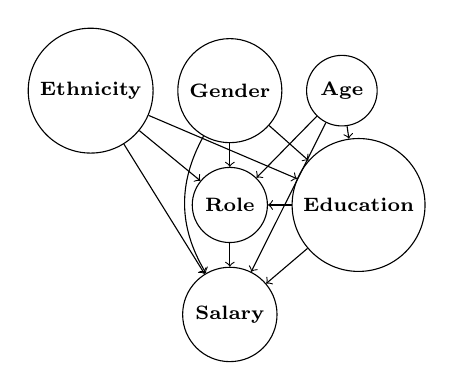
\begin{tikzpicture}[node distance=0.6cm and 1cm, every node/.style={minimum size=0.5cm}]
        \tikzset{vertex/.style = {draw, circle, align=center}}

        \node[vertex] (Ethnicity) {\bf\scriptsize{{Ethnicity}}};
        \node[vertex, right=0.3cm of Ethnicity] (Gender) {\bf{\scriptsize{Gender}}};
        \node[vertex, right=0.3cm of Gender] (Age) {\bf{\scriptsize{Age}}};
        \node[vertex, below=0.3cm of Gender] (Role) {\bf{\scriptsize{Role}}};
        \node[vertex, right=0.3cm of Role] (Education) {\bf{\small{\scriptsize{Education}}}};
        \node[vertex, below=0.3cm of Role] (Salary) {\bf{\scriptsize{Salary}}};

        \draw[->] (Ethnicity) -- (Salary);
        \draw[->] (Gender) -- (Role);
        \draw[->] (Age) -- (Role);
         \draw[->] (Education) -- (Role);
           \draw[->] (Education) -- (Salary);
             \draw[->] (Ethnicity) -- (Education);
                \draw[->] (Ethnicity) -- (Role);
             \draw[->] (Gender) -- (Education);
               \draw[->] (Age) -- (Education);
                 \draw[->] (Role) -- (Salary);
        \draw[->] (Gender) to[bend right] (Salary);
        \draw[->] (Age) -- (Salary);
    \end{tikzpicture}
    \caption{Partial causal DAG for the Stack Overflow dataset.}
    \label{fig:causal_DAG}
\end{figure}



 \begin{example}
Figure \ref{fig:causal_DAG} depicts a partial causal DAG for the SO dataset over the attributes in Table \ref{tab:data} as endogenous variables (we use a larger causal DAG with all 20 attributes in our experiments). 
  Given this causal DAG, we can observe that the role that a coder has in their company depends on their education, age gender and ethnicity.
\end{example}
\par


\par
\paratitle{Intervention} In Pearl's model, a treatment $T = t$ (on one or more variables) is considered as an {\em intervention} to a causal DAG by mechanically changing the DAG such that the values of node(s) of $T$ in $G$ are set to the value(s) in $t$, which is denoted by $\doop(T = t)$. Following this operation, the probability distribution of the nodes in the graph changes as the treatment nodes no longer depend on the values of their parents. Pearl's model gives an approach to estimate the new probability distribution by identifying the confounding factors $Z$ described earlier using conditions such as {\em d-separation} and {\em backdoor criteria} \cite{pearl2009causal}, which we do not discuss in this paper.


\par
\paratitle{Average Treatment Effect} The effects of an intervention are often measured by evaluating
% \par
% \paratitle{Causal inference, Treatment, ATE, and CATE}
% \newtextold{One of the primary goals  of {\em causal inference} is to estimate the effect of making a change in terms of a {\em treatment} $T$ (often referred to as an intervention)
% on the outcome $O$. 
% %A variable that is modified is often referred to as the treatment variable $T$ and the metric used to captures 
% The effect of treatment $T$ on outcome $O$ is measured by 
% %is known as 
{\em Conditional Average treatment effect (CATE)}, 
%a {\em treatment variable} $T$ on an outcome variable $O$ (e.g., what is the effect of higher \verb|Education| on \verb|Salary|). 
measuring the effect of an intervention on a subset of records~\cite{rubin1971use,holland1986statistics} by calculating the difference in average outcomes between the group that receives the treatment and the group that does not (called the {\em control} group), providing an estimate of how the intervention by $T$ influences an outcome $O$ for a given subpopulation. 
% Mathematically,
% \begin{equation}
%     %{\small ATE(T,O) = \mathbb{E}[O \mid \doop(T=1)] -      \mathbb{E}[O \mid \doop(T=0)]}
%     {\small ATE(T, O) = \mathbb{E}[O \mid \doop(T=1)] -  
%     \mathbb{E}[O \mid \doop(T=0)]}
% \label{eq:ate}
% \end{equation}
% In our work, where the treatment with maximum effect may vary among different subpopulations, we are interested in computing the \emph{Conditional Average Treatment Effect} (CATE), which measures the effect of a treatment on an outcome on \emph{a subset of input units}~\cite{rubin1971use,holland1986statistics}. 
Given a subset of the records defined by (a vector of) attributes $B$ and their values $b$, 
%g {\in} \Qagg(\db)$ defined by a predicate $G {=} g$ 
we can compute $CATE(T,O \mid B = b)$ as:
{
\begin{eqnarray}    
    %CATE(T,O \mid G=g) = \mathbb{E}[O \mid \doop(T=1)&, G=g] -  \mathbb{E}[O \mid \doop(T=0), G=g] 
   % CATE(T,O \mid B = b) = 
    \mathbb{E}[O \mid \doop(T=1), B = b] -  
    \mathbb{E}[O \mid \doop(T=0), B = b]\label{eq:cate}
\end{eqnarray}
}
Setting $B=\phi$ is equivalent to the ATE estimate.
The above definitions assumes that the treatment assigned to one unit does not affect the outcome of another unit (called the {Stable Unit Treatment Value Assumption (SUTVA)) \cite{rubin2005causal}}\footnote{This assumption does not hold for causal inference on multiple tables and even on a single table where tuples depend on each other.}. 


The ideal way of estimating the ATE and CATE is through {\em randomized controlled experiments}, 
where the population is randomly divided into two groups (treated and control, for binary treatments): 
%treated group that receives the treatment and control group that does not (denoted by 
%{the \em treated} group 
denoted by 
$\doop(T = 1)$ 
%for a binary treatment)  (the {\em control} group, 
and $\doop(T = 0)$ resp.)~\cite{pearl2009causal}.
%\sr{edited up to here, going to read the rest first, this section should not look like causumx}
%\par
%\par
However, randomized experiments cannot always be performed due to ethical or feasibility issues. In these scenarios, observational data is used to estimate the treatment effect, which requires the following additional assumptions. 
% {\em Observational Causal Analysis} still allows sound causal inference under additional assumptions. Randomization in controlled trials mitigates the effect of {\em confounding factors}, i.e., attributes that can affect the treatment assignment and outcome. Suppose we want to understand the causal effect of \verb|Education| on \verb|Salary| from the SO dataset.  %in Example~\ref{ex:running_example}. 
% We no longer apply Eq. (\ref{eq:ate}) since the values of \verb|Education| were not assigned at random in this data, and obtaining higher education largely depends on other attributes like \verb|Gender|, \verb|Age|, and \verb|Country|. 
% Pearl's model provides ways to account for these confounding attributes $Z$ to get an unbiased causal estimate from observational data under the following assumptions ($\independent$ denotes independence):
% \vspace{-2mm}
\newtextold{
The first assumption is called {\em unconfoundedness} or {\em strong ignorability}  \cite{rosenbaum1983central} says that the independence of outcome $O$ and treatment $T$ conditioning on a set of confounder variables  (covariates) $Z$, i.e.,
%\begin{eqnarray}
 $    O \independent T | Z {=} z$.
 %\label{eq:unconfoundedness}
%\end{eqnarray}
The second assumption called {\em overlap or positivity} says that there is a chance of observing individuals in both the treatment and control groups for every combination of covariate values, i.e., 
%\begin{eqnarray}
   $ 0 < Pr(T {=} 1 ~~|~~Z {=} z)< 1 $.
   %\label{eq:overlap}
%\end{eqnarray}
}
%\sg{Is this overlap or positivity? maybe both are the same?} \sr{yeah - same - from Google AI - The overlap assumption, also known as the positivity assumption, is a key assumption in causal inference that states that there is a chance of observing individuals in both the treatment and control groups for every combination of covariate values.}
% The above conditions are known as {\em Strong Ignorability} in Rubin's model \cite{rubin2005causal}.
The unconfoundedness assumption requires that the treatment $T$ and the outcome $O$ be independent when conditioned on a set of variables $Z$. In SO, assuming that only $Z$ =\{\verb|Gender|, \verb|Age|, \verb|Country|\} affects $T = $ \verb|Education|, if we condition on a fixed set of values of $Z$, i.e., consider people of a given gender, from a given country, and at a given age, then $T = $ \verb|Education| and $O = $ \verb|Salary| are independent. For such confounding factors $Z$,  Eq. (\ref{eq:cate}) reduces to the following form 
(positivity 
gives the feasibility of the expectation difference): 
 \vspace{-1mm}
{\small
\begin{flalign}    
% \begin{eqnarray}
   % % & ATE(T,O) = \mathbb{E}_Z \left[\mathbb{E}[O \mid T=1, Z = z] -  
   %  \mathbb{E}[O \mid T=0, Z = z] \right] \label{eq:conf-ate}\\
 & CATE(T,O {\mid} B {=} b) {=} \nonumber
    \mathbb{E}_Z \left[\mathbb{E}[O {\mid} T{=}1, B {=} b, Z {=} z] {-}  
    \mathbb{E}[O {\mid} T{=}0, B {=} b, Z {=} z]\right]\label{eq:conf-cate}
\end{flalign}
% \end{eqnarray}
}
% \vspace{-4mm}
This equation contains conditional probabilities and not $\doop(T = b)$, which can be estimated from an observed data. 
Pearl's model gives a systematic way to find such a $Z$ when a causal DAG is available. 




\section{An Analysis of Enumeration in OMT}%
\label{sec:analysis}

As described in~\sref{sec:omt-solving}, a basic \omt{} solving schema involves
the interaction of a combinatorial and a theory-specific optimization
components. In the combinatorial component, a \smt{} solver enumerates
\T{}-satisfiable truth assignments that propositionally satisfy the problem
formula $\vi$ conjoined with increasingly tighter bounds on the cost of the
optimum solution. In the theory-specific component, a \T-minimizer finds a
\T{}-model of minimum cost within the constraints imposed by the given truth
assignment. This model is then used to tighten the upper bound for the cost of
the optimum model and continue the search, until the formula is found
unsatisfiable.

Since the enumeration is based on the CDCL(\T) schema~\cite{marques-silvaConflictDrivenClauseLearning2021},
these truth assignments are typically \emph{total}, i.e., they assign a truth value to
each atom of the formula. %In the following example, we illustrate how this can
%
% be suboptimal in many cases, 
% causing an unnecessary increase in the number of
% search iterations.
%
However, we point out that total truth assignments can often over-constrain the search space for the optimum model, whereas relying on \emph{partial} truth assignments can be much more effective. 
Intuitively,
\emph{by removing from the current satisfying truth
    assignment \T{}-constraints that are not strictly necessary for the propositional
    satisfaction of the formula, we enlarge the area within which the optimum model
    is searched, thus increasing the chances of finding a better optimum model.}
%
This means that the solver can add a tighter upper bound
to the cost of the global optimum, potentially reducing the number of search
iterations needed to find it, and consequently the overall solving time.
Moreover, this improvement can be crucial for anytime OMT solving, as it allows
the solver to converge faster to better solutions within the given time limit.
% This concept is similar to the idea of pure-literal filtering (see~\sref{sec:bg:smt}), with the difference that this is performed only once a \T-satisfiable total truth assignment is found, and not only pur

%Following this observation, we investigated how applying
%assignment-reduction techniques to feed the
We illustrate this idea in the following example.
% \T-minimizer with short partial
% models can improve the effectiveness of the \omt{} search.
% by adapting truth-assignment minimization techniques to the \omlarat{} framework.

% \subsection{OMT with partial assignments}%
% \label{sec:approach:linear-search}

\begin{figure}[t]
    %
% --- inline annotations
%
\newcommand{\red}[1]{{\color{red}#1}}
\newcommand{\todo}[1]{{\color{red}#1}}
\newcommand{\TODO}[1]{\textbf{\color{red}[TODO: #1]}}
% --- disable by uncommenting  
% \renewcommand{\TODO}[1]{}
% \renewcommand{\todo}[1]{#1}



\newcommand{\VLM}{LVLM\xspace} 
\newcommand{\ours}{PeKit\xspace}
\newcommand{\yollava}{Yo’LLaVA\xspace}

\newcommand{\thisismy}{This-Is-My-Img\xspace}
\newcommand{\myparagraph}[1]{\noindent\textbf{#1}}
\newcommand{\vdoro}[1]{{\color[rgb]{0.4, 0.18, 0.78} {[V] #1}}}
% --- disable by uncommenting  
% \renewcommand{\TODO}[1]{}
% \renewcommand{\todo}[1]{#1}
\usepackage{slashbox}
% Vectors
\newcommand{\bB}{\mathcal{B}}
\newcommand{\bw}{\mathbf{w}}
\newcommand{\bs}{\mathbf{s}}
\newcommand{\bo}{\mathbf{o}}
\newcommand{\bn}{\mathbf{n}}
\newcommand{\bc}{\mathbf{c}}
\newcommand{\bp}{\mathbf{p}}
\newcommand{\bS}{\mathbf{S}}
\newcommand{\bk}{\mathbf{k}}
\newcommand{\bmu}{\boldsymbol{\mu}}
\newcommand{\bx}{\mathbf{x}}
\newcommand{\bg}{\mathbf{g}}
\newcommand{\be}{\mathbf{e}}
\newcommand{\bX}{\mathbf{X}}
\newcommand{\by}{\mathbf{y}}
\newcommand{\bv}{\mathbf{v}}
\newcommand{\bz}{\mathbf{z}}
\newcommand{\bq}{\mathbf{q}}
\newcommand{\bff}{\mathbf{f}}
\newcommand{\bu}{\mathbf{u}}
\newcommand{\bh}{\mathbf{h}}
\newcommand{\bb}{\mathbf{b}}

\newcommand{\rone}{\textcolor{green}{R1}}
\newcommand{\rtwo}{\textcolor{orange}{R2}}
\newcommand{\rthree}{\textcolor{red}{R3}}
\usepackage{amsmath}
%\usepackage{arydshln}
\DeclareMathOperator{\similarity}{sim}
\DeclareMathOperator{\AvgPool}{AvgPool}

\newcommand{\argmax}{\mathop{\mathrm{argmax}}}     


    \centering
    \begin{subfigure}{0.33\textwidth}%
        \resizebox{\columnwidth}{!}{\begin{tikzpicture}
    \path (0,0) pic {planes};
    % fill
    \fill[plane, opacity=\planeopacity] (BL) -- (TL) -- (TR) -- cycle;
    \fill[plane, opacity=\planeopacity] (13/3,\mY) -- (2, \MY) -- (TL) -- (BL) -- cycle;
    \fill[plane, opacity=\planeopacity] (\mX,2) -- (\MX, 2) -- (BR) -- (BL) -- cycle;
    \fill[plane, opacity=\planeopacity] (-2,\mY) -- (BR) -- (TR) -- (-2,\MY) -- cycle;
    \fill[plane, opacity=\planeopacity] (4,\MY) -- (4, \mY) -- (BL) -- (TL) -- cycle;
    %lines
    \draw[dashed, name path=plane1] (BL) -- (TR) node[above left] {\LARGE$2x-3y\leq 6$};
    \draw[dashed, name path=plane2] ( 13/3,\mY) -- (2, \MY) node[above] {\LARGE$y \leq -3x + 9$};
    \draw[dashed, name path=plane3] (-3, 2) -- (23/3, 2) node[below left] {\LARGE$y \leq 2$};
    \draw[dashed, name path=plane4] (-2,3) -- (-2,-4) node[below] {\LARGE$\neg(x < -2)$};
    \draw[dashed, name path=plane5] (4,\MY) -- ( 4,\mY) node[below] {\LARGE$x \leq 4$};
    % Compute intersection points
    \path[name intersections={of=plane3 and plane4, by={A}}];
    \path[name intersections={of=plane2 and plane3, by={B}}];
    \path[name intersections={of=plane5 and plane3, by={C}}];
    \path[name intersections={of=plane1 and plane3, by={D}}];
    \path[name intersections={of=plane1 and plane5, by={E}}];
    \path[name intersections={of=plane1 and plane2, by={F}}];
    \path[name intersections={of=plane1 and plane4, by={G}}];
    % Draw bold lines around the intersection
    \draw[very thick] (A) -- (B) -- (F) -- (G) -- cycle;
    % Draw the intersection polygon
    \fill[opacity=.4, top color=white, bottom color=blue, shading angle=64.76] (A) -- (B) -- (F) -- (G) -- cycle;
    % optimum point
    \path (0,0) pic {axes};
    \draw[fill=red]   (F) circle (1.5mm);
\end{tikzpicture}}%
        \caption{Total assignment $\mu$~\eqref{eq:omt-partial-assignments:total-assignment:mu}}%
        \label{fig:omt-partial-assignments:step1}%
    \end{subfigure}%
    \begin{subfigure}{0.33\textwidth}%
        \resizebox{\columnwidth}{!}{\begin{tikzpicture}
    % Draw the Cartesian plane
    \path (0,0) pic {planes};
    % fill
    \fill[plane, opacity=\planeopacity] (BL) -- (TL) -- (TR) -- cycle;
    %   \fill[plane, opacity=\planeopacity] (13/3,\mY) -- (2, \MY) -- (TL) -- (BL) -- cycle;
    \fill[plane, opacity=\planeopacity] (\mX,2) -- (\MX, 2) -- (BR) -- (BL) -- cycle;
    \fill[plane, opacity=\planeopacity] (-2,\mY) -- (BR) -- (TR) -- (-2,\MY) -- cycle;
    \fill[plane, opacity=\planeopacity] (4,\MY) -- (4, \mY) -- (BL) -- (TL) -- cycle;
    % lines
    \draw[dashed, name path=plane1] (BL) -- (TR) node[above left] {\LARGE$2x-3y\leq 6$};
    \draw[dashed, name path=plane2, opacity=0.3] ( 13/3,\mY) -- (2, \MY) node[above] {\LARGE$y \leq -3x + 9$};
    \draw[dashed, name path=plane3] (-3, 2) -- (23/3, 2) node[below left] {\LARGE$y \leq 2$};
    \draw[dashed, name path=plane4] (-2,3) -- (-2,-4) node[below] {\LARGE$\neg(x < -2)$};
    \draw[dashed, name path=plane5] (4,\MY) -- ( 4,\mY) node[below] {\LARGE$x \leq 4$};
    % Compute intersection points
    \path[name intersections={of=plane3 and plane4, by={A}}];
    \path[name intersections={of=plane2 and plane3, by={B}}];
    \path[name intersections={of=plane5 and plane3, by={C}}];
    \path[name intersections={of=plane1 and plane3, by={D}}];
    \path[name intersections={of=plane1 and plane5, by={E}}];
    \path[name intersections={of=plane1 and plane2, by={F}}];
    \path[name intersections={of=plane1 and plane4, by={G}}];
    % Draw bold lines around the intersection
    \draw[very thick] (A) -- (C) -- (E) -- (G) -- cycle;
    % Draw the intersection polygon
    \fill[opacity=.4, top color=white, bottom color=blue, shading angle=64.76] (A) -- (C) -- (E) -- (G) -- cycle;
    \path (0,0) pic {axes};
    \draw[fill=red]   (E) circle (1.5mm);
\end{tikzpicture}}%
        \caption{Partial assignment $\muprime$~\eqref{eq:omt-partial-assignments:total-assignment:muprime}}%
        \label{fig:omt-partial-assignments:step2}%        
    \end{subfigure}%
    \begin{subfigure}{0.33\textwidth}%
        \resizebox{\columnwidth}{!}{\begin{tikzpicture}
    \path (0,0) pic {planes};
    % fill
    \fill[plane, opacity=\planeopacity] (BL) -- (TL) -- (TR) -- cycle;
    %   \fill[plane, opacity=\planeopacity] (13/3,\mY) -- (2, \MY) -- (TL) -- (BL) -- cycle;
    \fill[plane, opacity=\planeopacity] (\mX,2) -- (\MX, 2) -- (BR) -- (BL) -- cycle;
    \fill[plane, opacity=\planeopacity] (-2,\mY) -- (BR) -- (TR) -- (-2,\MY) -- cycle;
    %    \fill[plane, opacity=\planeopacity] (4,\MY) -- (4, \mY) -- (BL) -- (TL) -- cycle;
    % lines
    \draw[dashed, name path=plane1] (BL) -- (TR) node[above left] {\LARGE$2x-3y\leq 6$};
    \draw[dashed, name path=plane2, opacity=0.3] ( 13/3,\mY) -- (2, \MY) node[above] {\LARGE$y \leq -3x + 9$};
    \draw[dashed, name path=plane3] (-3, 2) -- (23/3, 2) node[below left] {\LARGE$y \leq 2$};
    \draw[dashed, name path=plane4] (-2,3) -- (-2,-4) node[below] {\LARGE$\neg(x < -2)$};
    \draw[dashed, name path=plane5, opacity=0.3] (4,\MY) -- ( 4,\mY) node[below] {\LARGE$x \leq 4$};
    % Compute intersection points
    \path[name intersections={of=plane3 and plane4, by={A}}];
    \path[name intersections={of=plane2 and plane3, by={B}}];
    \path[name intersections={of=plane5 and plane3, by={C}}];
    \path[name intersections={of=plane1 and plane3, by={D}}];
    \path[name intersections={of=plane1 and plane5, by={E}}];
    \path[name intersections={of=plane1 and plane2, by={F}}];
    \path[name intersections={of=plane1 and plane4, by={G}}];
    % Draw bold lines around the intersection
    \draw[very thick] (A) -- (C) -- (D) -- (G) -- cycle;
    % Draw the intersection polygon
    \fill[opacity=.4, top color=white, bottom color=blue, shading angle=64.76] (A) -- (D) -- (G) -- cycle;
    \path (0,0) pic {axes};
    \draw[fill=red]   (D) circle (1.5mm);
\end{tikzpicture}}
        \caption{Partial assignment $\mupprime$~\eqref{eq:omt-partial-assignments:total-assignment:mupprime}}%
        \label{fig:omt-partial-assignments:step3}%        
    \end{subfigure}%
    \caption{
        Graphical representation of~\Cref{ex:omt-partial-assignments}. For each step, the half-planes representing the constraints in the truth assignment are delimited by dashed lines and colored in grey. The intersection of these constraints is colored in blue, with a gradient that follows the value of $\obj$ (the lower the value of $\obj$, the more intense the color), and the red dot represents the optimum model found within this region.
    }%
    \label{fig:omt-partial-assignments}%
\end{figure}

\begin{example}%
    \label{ex:omt-partial-assignments}
    Consider the \omlarat{} problem \pair{\vi}{\obj} where \vi{} is the formula in~\eqref{eq:smt} in~\Cref{ex:smt}, and $\obj\defas -2x$.
    Consider the following scenario, which is graphically represented in~\Cref{fig:omt-partial-assignments}. Consider the \larat{}-satisfiable total truth assignment that propositionally satisfies $\vi$:
    \begin{equation}%
        \label{eq:omt-partial-assignments:total-assignment:mu}
        \mu\defas\set{(2x-3y\leq 6),(y\leq 2),\neg(x<-2),(y\leq-3x+9),(x\leq 4)}.
    \end{equation} 
    The optimum model of $\mu$ is \set{x\mapsto{}3,y\mapsto{}0} with $\obj=-6$ (\Cref{fig:omt-partial-assignments:step1}). % This cost is then used to tighten the upper bound by adding the constraint $(\obj < -6)$ and continue the search. 
    We notice, however, that, e.g., the constraint $(y\leq-3x+9)$ is not strictly necessary for propositionally satisfying $\vi$, as $\vi$ is satisfied also by:
    \begin{equation}%
        \label{eq:omt-partial-assignments:total-assignment:muprime}
        \muprime\defas\mu\setminus\set{(y\leq-3x+9)}=\set{(2x-3y\leq 6),(y\leq 2),\neg(x<-2),(x\leq 4)}.
    \end{equation}
    %Suppose, instead, that we drop the unnecessary constraint $(y\leq-3x+9)$ from $\mu$. 
    The optimum model of $\muprime$ is \set{x\mapsto{}4,y\mapsto{}2/3} with
    $\obj=-8$ (\Cref{fig:omt-partial-assignments:step2}).
    %
    If we further remove the unnecessary constraint $(x \leq 4)$, then we obtain
    \begin{equation}%
        \label{eq:omt-partial-assignments:total-assignment:mupprime}
        \mupprime\defas\muprime\setminus\set{(x \leq
        4)}=\set{(2x-3y\leq 6),(y\leq 2),\neg(x<-2)}
    \end{equation}
    with optimum model \set{x\mapsto{}6,y\mapsto{}2} and $\obj=-12$ (\Cref{fig:omt-partial-assignments:step3}). Finally, we could remove
    either $\neg(x<-2)$ or $(y\leq 2)$. In the first case, we would obtain a
    partial truth assignment with the same optimum model as $\mupprime$, since the
    constraint does not ``oppose'' to the optimization of $\obj$ in \mupprime. In the second
    case, instead, by removing $(y\leq 2)$ we would obtain an assignment where the value of
    \obj{} is unbounded, and the optimum model has $\obj=-\infty$.
\end{example}

In general, partial truth assignments have an optimum model that is necessarily better or equal to that of the total truth assignments extending them. Since multiple partial truth assignments can be obtained from a total one, the choice of which constraints to drop can be crucial to improve the quality of the optimum model found.
\section{Exploiting Partial Truth Assignments in OMT}%
\label{sec:approach}
\begin{algorithm}[t]
    \newcommand{\res}{\textsf{res}}
    \begin{algorithmic}[1]
        %\begin{rschange}
        \caption[A]{{\sc Linear-search OMT with partial assignments}($\vi, \obj$)\\
            \hspace*{\algorithmicindent}\textbf{Input}:
            Formula $\vi$, objective $\obj$\\
            \hspace*{\algorithmicindent}\textbf{Output}: $\satres/\unsatres$, optimum model $\M$}%
        \label{alg:omt-partial}
        \STATE \makebox[.5cm][c]{$\M$}$\gets \emptyset$ \algorithmiccomment{Best model found so far}
        \STATE \makebox[.5cm][c]{$\ub$}$\gets \infty$ \algorithmiccomment{Current upper bound}
        \STATE \makebox[.5cm][c]{$\res$}$\gets \satres$ \algorithmiccomment{Status of the search}
        \WHILE{$\res = \satres$}
        \STATE $\tuple{\res,\eta} \gets \incrementalsmt(\vi\wedge(\obj<\ub))$
        \IF{$\res = \satres$}
        \STATE\label{alg:line:omt-partial:minimize} \makebox[.5cm][c]{$\color{blue}\mu$}$\color{blue}\gets\omtminimizeassignment(\vi,\eta,\obj)$
        \STATE \makebox[.5cm][c]{$\M$}$\gets \minimize(\mu,\obj)$
        \STATE \makebox[.5cm][c]{$\ub$}$\gets \M(\obj)$
        \ENDIF
        \ENDWHILE
        \IF{$\M = \emptyset$}
        \RETURN $\tuple{\unsatres,\emptyset}$
        \ELSE
        \RETURN $\tuple{\satres,\M}$
        \ENDIF
    \end{algorithmic}
\end{algorithm}

The general schema of our approach is presented in~\Cref{alg:omt-partial}. This
algorithm is a variant of the basic \omt{} linear-search
schema~\cite{sebastianiOptimizationSMTLAQ2012,sebastianiOptimizationModuloTheories2015}
described in~\sref{sec:bg:omt}. The main difference is the call to the
$\omtminimizeassignment$ procedure (line~\ref{alg:line:omt-partial:minimize}),
which is responsible for reducing the truth assignment to be fed to the
\T-minimizer, provided that the resulting partial truth assignment still
propositionally satisfies the formula. Depending on the implementation of this
procedure, the assignment-reduction strategy can be more or less effective in
improving the search for the global optimum.

In \sref{sec:approach:basic-assignment-minimization} and
\sref{sec:approach:guided-assignment-minimization}, we describe two possible
implementations of this procedure.

% \TODO{Say something about correctness of the approach?}
% \TODO{Say something about relation with pure-literal filtering?}

\subsection{Basic Assignment Reduction}%
\label{sec:approach:basic-assignment-minimization}

The first approach is to reduce the truth assignment using~\Cref{alg:minimize}
in~\sref{sec:bg:partial-truth-assignments}, i.e., iterating over all the
literals in the current truth assignment $\eta$, and dropping them one by one,
if possible.
%This approach is simple and general, but it may not be effective in practice, as it does not take into account the properties of the \omt{} search strategy.
A straightforward improvement is to only try to drop \T-literals, since they
are the ones that, if dropped, can potentially enlarge the area within which
the optimum \T-model is searched. This procedure is simple and general, and
comes with a limited overhead, as each truth assignment is scanned only once to
find the literals to drop, and the \T-minimizer is called only once for each
candidate assignment.

This approach, however, might not be very effective in practice, as it ``blindly''
removes literals from the truth assignment without taking into account the
properties of the \omt{} search strategy. In particular, it may drop literals that
are not relevant for the optimization, enlarging the search area in the wrong
direction, possibly preventing from dropping other literals that are more
relevant.%does not take

\subsection{OMT-Guided Assignment Reduction}%
\label{sec:approach:guided-assignment-minimization}
%The main limitation of the previous approach is that the heuristics used to choose the atoms to leave unassigned do not take into account the properties of the \omt{} search strategy. 
We propose an ad-hoc assignment-reduction technique for \omt{} solving, which
is outlined in~\Cref{alg:omt-minimize-assignment-guided}.
%
%address these points.
%investigate \emph{on-demand} truth assignment minimization.
% By this term, we mean that, once a \larat-satisfiable satisfying (partial) truth assignment has been found, and the \larat-minimizer has found a minimal model within the corresponding area, then we can try to remove just some of the \larat-atoms and look if a better model exists within the new enlarged area. Moreover, since both the constraints and the cost function are linear, by the simplex method
% the optimum model lies on a vertex of the polytope. As an heuristic, we can choose to drop one of the constraints that form the vertex, since a better model is likely to be found in that portion of space. 
%
%
Suppose that, after the \T-minimizer has found a minimum model within the
current truth assignment $\mu$
(line~\ref{alg:omt-minimize-assignment-guided:line:minimize1}), it returns also
one (or more) literal(s) that limit the current minimum
(line~\ref{alg:omt-minimize-assignment-guided:line:propose1}). These literals
are part of some (possibly minimal) $\muprime\subseteq\mu$ such that
$\muprime\cup\set{\obj<\M(\obj)}$ is \T-unsatisfiable. Intuitively, the removal
of any literal $\ell\in\muprime$ is very likely to lead to a better optimum model,
provided that $\mu\setminus\set{\ell}$ still propositionally satisfies $\vi$
(line~\ref{alg:omt-minimize-assignment-guided:line:ifcandrop}).%the list of the literals%This corresponds to a minimal 

%these literals, if dropped, are likely
%to lead to a better optimum model. 
We can then iteratively drop these literals and re-run the \T-minimizer, until
no more literals can be dropped
(lines~\ref{alg:omt-minimize-assignment-guided:line:while}--\ref{alg:omt-minimize-assignment-guided:line:propose2}).
\begin{algorithm}[t]
    \begin{algorithmic}[1]
        %\begin{rschange}
        \caption[A]{\omtminimizeassignmentguided($\vi, \eta$, $\obj$)\\
            \hspace*{\algorithmicindent}\textbf{Input}:
            Formula $\vi$, \T-satisfiable total truth assignment $\eta$ satisfying $\vi$, objective $\obj$\\
            \hspace*{\algorithmicindent}\textbf{Output}: Reduced truth assignment $\mu\subseteq\eta$ satisfying $\vi$}%
        \label{alg:omt-minimize-assignment-guided}
        \STATE\makebox[.5cm][c]{$\mu$}$\gets\eta$
        \STATE\makebox[.5cm][c]{$\M$}$\gets\minimize(\mu,\obj)$\label{alg:omt-minimize-assignment-guided:line:minimize1}
        \STATE\makebox[.5cm][c]{$\ell$}$\gets\proposelit()$\label{alg:omt-minimize-assignment-guided:line:propose1}
        \WHILE{$\ell\neq\bot$}\label{alg:omt-minimize-assignment-guided:line:while}
        \IF{$\mu\setminus\set{\ell}$ satisfies all clauses in $\vi$}\label{alg:omt-minimize-assignment-guided:line:ifcandrop}
        \STATE \makebox[.5cm][c]{$\mu$}$\gets \mu \setminus \set{\ell}$\label{alg:omt-minimize-assignment-guided:line:drop}
        %\STATE $\tpop(\ell)$\label{alg:omt-minimize-assignment-guided:line:tpop}
        \STATE \makebox[.5cm][c]{$\M$}$\gets\minimize(\mu,\obj)$\label{alg:omt-minimize-assignment-guided:line:minimize2}
        \ENDIF
        \STATE $\ell\gets\proposelit()$\label{alg:omt-minimize-assignment-guided:line:propose2}
        \ENDWHILE
        \RETURN $\mu$
    \end{algorithmic}
\end{algorithm}

We describe a possible implementation of the $\proposelit$ procedure
in~\Cref{alg:omt-minimize-assignment-guided} for the case of \omlarat{}.
%
As we have seen in~\sref{sec:bg:omt}, a \larat{}-minimizer can be implemented
as a variant of the Simplex
method~\cite{dutertreFastLinearArithmeticSolver2006,sebastianiOptimizationSMTLAQ2012},
by which an optimum model is always found on a vertex of the polytope defined
by the conjunction of \larat-constraints on which it is invoked. Thus, in this
case, the candidate constraints to be dropped are those that form such vertex.
This information can be easily obtained from the Simplex tableau~\cite{dutertreFastLinearArithmeticSolver2006}.
%  \TODO{Find a way to easily explain this.\\
%  The tableau stores
%  $x_i = bi + \sum_{x_j\in\N} a_{i,j}x_j$, forall $x_i\in\B$\\
%  and then it keeps track of the bounds for each variable $l_i\leq x_i\leq u_i$\\
%  Basically, we look for $x_i\in\N$ such that\\
%  $\beta[x_i] = u_i$ and $a_{\obj,i} < 0$\\
%  $\beta[x_i] = l_i$ and $a_{\obj,i} > 0$\\
%  where $\beta[x_i]$ is the current value of $x_i$.\\
%  For each such $x_i$, we get the constraint imposing the
%  bound.
%  }

For other theories, the implementation of the $\proposelit$ procedure may be
more complex, requiring the extraction of a (possibly minimal) conflict set of $\mu\cup\set{\obj<\M(\obj)}$.
In general, also heuristic strategies can be used, as they only
provide suggestions to the assignment-reduction procedure, and do not affect
the correctness of the search.

Regarding the computational cost, the proposed approach can be more expensive than
the basic assignment reduction, as it requires the \T-minimizer to be called
multiple times. \T-minimizers, however, are typically designed to be called
incrementally, maintaining the state of the previous calls, and thus the
overhead of multiple calls is limited.
% \GMSIDENOTE{Remove or expand?}
% Another possible source of complexity is that the incrementality of \T-minimizer is based on a stack interface, whereas
% \omtminimizeassignmentguided{} requires to drop any literal in the assignment,
% which may require a more complex data structure to be implemented efficiently.

\section{Experiments}
\label{sec:Experiments}
We first demonstrate the effectiveness of rule-based metrics (\S\ref{sec: Features Comparison}) and ScholarDetect models (\S\ref{sec:ScholarDetect Evaluation}) in \texttt{LLMetrica}, then apply these methods to real-world conference data to assess and predict LLM penetration trends (\S\ref{sec:Temporal Analysis}). Finally, case studies are used to explore the specific differences between human-written and LLM-generated content (\S\ref{sec: Case Study}).

% case studies provide deeper insights into the distinguishing features of human-written vs. LLM-generated content (\S\ref{sec: Case Study}).

% we conduct case studies to gain deeper insights into the distinctive characteristics of human-written and LLM-generated content (\S\ref{sec: Case Study}).





\subsection{Features Comparison: Human vs LLM}
\label{sec: Features Comparison}
We apply the proposed rule-based metrics (\S\ref{sec:metric}) to  \texttt{ScholarLens} to compare the features of human-written and LLM-generated texts, and find that the feature preferences of LLM-generated texts can be effectively compared and evaluated.

% Results are shown in Figure~\ref{fig:compare_general} (general features) and Figure~\ref{fig:compare_specific} (specific features).


% Please add the following required packages to your document preamble:
% \usepackage{multirow}
% \begin{table*}[]
% \begin{tabular}{c|c|ccc|ccc|ccc}
% \hline
% \multirow{2}{*}{}         & \multirow{2}{*}{Model} & \multicolumn{3}{c|}{Abstract} & \multicolumn{3}{c|}{Meta-Reivew} & \multicolumn{3}{c}{Reiview}                  \\ \cline{3-11} 
%                           &                        & Human   & LLM     & Overall   & Human    & LLM      & Overall    & Human & LLM   & \multicolumn{1}{c|}{Overall} \\ \cline{2-11} 
% \multirow{3}{*}{Baseline} & MAGE                   & 64.46   & 37.07   & 54.58     & 65.80    & 28.34    & 53.70      & 92.98 & 57.60 & \multicolumn{1}{c|}{87.95}   \\
%                           & RaiDetector            & 62.04   & 71.21   & 67.25     & 57.39    & 70.25    & 64.96      & 24.48 & 26.84 & \multicolumn{1}{c|}{25.68}   \\
%                           & HNDCDetector           & 54.59   & 85.85   & 78.43     & 62.63    & 76.74    & 71.33      & 86.39 & 54.90 & \multicolumn{1}{c|}{79.09}   \\ \hline
% \end{tabular}
% \caption{the F1 score performance of our fine-tuning model compare with two of current detect model}
% \label{tab:fine-detection}
% \end{table*}


% Please add the following required packages to your document preamble:
% \usepackage{booktabs}
% \usepackage{multirow}
\begin{table*}[t]
\centering
\scalebox{0.64}{
\begin{tabular}{@{}l|p{1.3cm}|rrr|rrr|rrr|r@{}}
\toprule
\multirow{2}{*}{\textbf{Model}}                                  & \multirow{2}{*}{\parbox{1.3cm}{\textbf{LLM Source}}} & \multicolumn{3}{c|}{\textbf{Abstract}}                          & \multicolumn{3}{c|}{\textbf{Meta-Review}}                       & \multicolumn{3}{c|}{\textbf{Review}}                            & \multicolumn{1}{l}{\multirow{2}{*}{\textbf{Avg.}}} \\ \cmidrule(lr){3-11}
                                                                 &   \multirow{1}{*}                     & Human               & LLM                 & Overall             & Human               & LLM                 & Overall             & Human               & LLM                 & Overall             & \multicolumn{1}{l}{}                                  \\ \midrule
\textbf{MAGE}                                                    & \multirow{3}{*}{-}                 & 40.62               & 35.14               & 38.00               & 40.58               & 33.43               & 37.21               & 92.98               & 57.60                & 87.95               & 54.39                                                 \\
\textbf{RAIDetect}                                               &                                    & 49.51               & 78.36               & 69.71               & 38.42               & 73.50                & 62.94               & 24.48               & 26.85               & 25.68               & 52.78                                                 \\
\textbf{HNDCDetect}                                              &                                    & 54.59               & 85.85               & 78.43               & 57.93               & 83.88               & 76.69               & 86.39               & 54.90                & 79.09               & 78.07                                                 \\ \midrule
\multirow{4}{*}{\textbf{$\text{ScholarDetect}_{\text{Abs}}$}}    & GPT-4o                             & 97.02\small ±0.50          & 99.02\small ±0.15          & 98.53\small ±0.23          & 87.65\small ±3.01          & 95.06\small ±1.48          & 92.95\small ±2.00          & 97.44\small ±0.20          & 79.97\small ±1.96          & 95.45\small ±0.37          & 95.64                                                 \\
                                                                 & Gemini                             & 84.40\small ±3.11          & 93.48\small ±1.59          & 90.80\small ±2.13          & 90.62\small ±1.98          & 95.06\small ±1.21          & 92.93\small ±1.63          & 96.41\small ±0.64          & 68.68\small ±7.26          & 93.56\small ±1.19          & 92.43                                                 \\
                                                                 & Claude                             & 91.61\small ±1.09          & 96.90\small ±0.46          & 95.47\small ±0.65          & 83.79\small ±4.74          & 93.02\small ±2.60          & 90.25\small ±3.40          & 95.69\small ±0.89          & 58.84\small ±12.55         & 92.20\small ±1.68          & 91.97                                                 \\
                                                                 & Mix                                & \underline{97.94\small ±0.16}          & \underline{99.32\small ±0.05}          & \underline{98.98\small ±0.07}          & 93.84\small ±0.23          & 97.81\small ±0.09          & 96.76\small ±0.13          & 97.56\small ±0.20          & 81.16\small ±1.92          & 95.68\small ±0.37          & 97.14                                                 \\ \midrule
\multirow{4}{*}{\textbf{$\text{ScholarDetect}_{\text{Meta}}$}}   & GPT-4o                             & 78.59\small ±1.64          & 90.47\small ±1.19          & 86.81\small ±1.45          & 99.53\small ±0.13          & 99.84\small ±0.04          & 99.76\small ±0.06          & 97.98\small ±0.21          & 84.95\small ±1.89          & 96.44\small ±0.39          & 94.34                                                 \\
                                                                 & Gemini                             & 80.13\small ±2.71          & 91.45\small ±1.56          & 88.05\small ±2.02          & 97.70\small ±1.86          & 99.19\small ±0.67          & 98.80\small ±0.98          & 97.65\small ±0.30          & 81.90\small ±2.69          & 95.83\small ±0.54          & 94.23                                                 \\
                                                                 & Claude                             & 62.42\small ±13.17         & 69.60\small ±16.38         & 66.93\small ±15.79         & 86.72\small ±7.94          & 94.15\small ±3.67          & 91.88\small ±5.02          & 97.82\small ±0.62          & 83.23\small ±5.56          & 96.14\small ±1.11          & 84.98                                                 \\
                                                                 & Mix                                & 84.20\small ±3.59          & 94.12\small ±2.24          & 91.47\small ±2.89          & \underline{99.84\small ±0.10}          & \underline{99.95\small ±0.03}          & \underline{99.92\small ±0.05}          & \textbf{99.52\small ±0.16} & \textbf{96.86\small ±1.08} & \textbf{99.17\small ±0.28} & 96.85                                                 \\ \midrule
\multirow{4}{*}{\textbf{$\text{ScholarDetect}_{\text{Hybrid}}$}} & GPT-4o                             & 97.69\small ±0.35          & 99.23\small ±0.13          & 98.84\small ±0.19          & 99.33\small ±0.17          & 99.78\small ±0.06          & 99.67\small ±0.08          & 97.73\small ±0.16          & 82.72\small ±1.42          & 95.98\small ±0.28          & \underline{98.16}                                                 \\
                                                                 & Gemini                             & 85.88\small ±0.19          & 94.32\small ±0.10          & 91.90\small ±0.13          & 97.84\small ±1.19          & 99.25\small ±0.43          & 98.89\small ±0.63          & 97.69\small ±0.31          & 82.29\small ±2.83          & 95.91\small ±0.56          & 95.56                                                 \\
                                                                 & Claude                             & 85.61\small ±1.67          & 94.11\small ±0.84          & 91.64\small ±1.13          & 96.49\small ±1.22          & 98.77\small ±0.44          & 98.18\small ±0.65          & 97.48\small ±0.26          & 80.35\small ±2.44          & 95.53\small ±0.47          & 95.13                                                 \\
                                                                 & Mix                                & \textbf{98.11\small ±0.35} & \textbf{99.37\small ±0.11} & \textbf{99.06\small ±0.17} & \textbf{99.88\small ±0.00} & \textbf{99.96\small ±0.00} & \textbf{99.94\small ±0.00} & \underline{98.06\small ±0.18}          & \underline{85.69\small ±1.53}          & \underline{96.59\small ±0.32}          & \textbf{98.53}                                        \\ \bottomrule
\end{tabular}}
\caption{Detection performance comparison of baseline models and ScholarDetect. \textbf{Bold} denotes the best performance, and \underline{underlined} denotes the second-best. ``Avg.'' shows the average overall score across the three test data types.}
\label{tab:fine-detection}
\end{table*}




\paragraph{General Linguistic Features}

Figure~\ref{fig:compare_general} shows trends in the characteristics of LLM-generated texts, with slight variations across different data types. Each metric reflects the consistency of features across texts generated by the three LLMs in at least one data type, demonstrating the `comparability' effectiveness of the chosen metrics.
Moreover, regardless of the data type or LLM used, LLM-generated texts consistently show higher values for Average Word Length (AWL) and Long Word Ratio (LWR), and lower values for Stopword Ratio (SWR) and Readability (FRE). This suggests that LLM-generated texts tend to use longer words, avoid excessive stopwords, and have lower readability.
For shorter text types, such as abstracts and meta-reviews, the observed increase in Type Token Ratio (TTR) reflects greater lexical diversity in LLM-generated texts.
This may be due to the conciseness inherent in short-form LLM-generated content. In contrast, for longer reviews, TTR decreases, potentially highlighting the limitations of LLMs in producing long-form content~\cite{wang-etal-2024-m4, wu2025survey}. Longer reviews may lack specificity~\cite{du-etal-2024-llms}, resulting in redundancy and repetitive segments.
Additionally, LLM-generated reviews tend to be more positive and subjective, suggesting a more favorable tone and less neutral objectivity. This aligns with \citet{jin-etal-2024-agentreview}, who found that LLM-generated reviews generally assign higher scores and show a higher acceptance rate.

\paragraph{Specific Semantic Features}
Figure~\ref{fig:compare_specific} shows the preferences of human-written and LLM-generated texts in both meta-reviews and reviews, based on four specific semantic features.
Notably, Since each LLM generates only one review per paper in \texttt{ScholarLens}, while each paper usually has multiple reviews, we combine reviews from all three LLMs into a unified set, so comparisons do not distinguish between them.
Comparative results show that LLM-generated meta-reviews exhibit higher semantic similarity to the referenced reviews, with lower sentence specificity.
This suggests that sentences within LLM-generated meta-reviews are more semantically similar to each other (prone to redundancy) and tend to mirror the content of the referenced reviews. 
A similar trend is observed for reviews, where the two specific features also show consistent patterns.
It is important to note that for the reviews, we assume all are LLM-generated in this experiment, which may amplify the differences in these semantic features. In reality, having more than two LLM-generated reviews per paper may be uncommon, which would likely reduce the observed disparity.

% Figure~\ref{fig:compare_specific} shows that LLM-generated meta-reviews exhibit higher semantic similarity to the referenced reviews. Additionally, the specificity of segments is lower, indicating that segments within LLM-generated meta-reviews are more semantically similar to each other (prone to redundancy) and tend to mirror the content of the referenced reviews. Similarly, for reviews, the trends observed in the two specific features are also consistent.
% It is important to note that for the reviews, we assume all are LLM-generated in this experiment, which may amplify the differences in the two semantic features. In reality, having more than two LLM-generated reviews per paper is rare, which would likely reduce the observed disparity.


\begin{figure}[t]
    \centering
    \begin{minipage}{0.55\linewidth}
        \centering
        \includegraphics[width=\linewidth]{fig/meta_specific_compare.pdf}
        \captionsetup{font=footnotesize}
        \subcaption{Meta-Review}
    \end{minipage}
    \hfill
    \begin{minipage}{0.4\linewidth}
        \centering
        \includegraphics[width=\linewidth]{fig/review_specific_compare.pdf}
        \captionsetup{font=footnotesize}
        \subcaption{Review}
    \end{minipage}
    \hfill
    \caption{Comparison of Human-Written and LLM-Generated Text Based on \textbf{Specific features} for Review and Meta-Review.}
    \label{fig:compare_specific}
\end{figure}
% AgentReview~\cite{jin-etal-2024-agentreview}.

\subsection{ScholarDetect Evaluation: Detectability}
\label{sec:ScholarDetect Evaluation}
We evaluate the trained model-based detectors, ScholarDetect (\S\ref{sec:detectors}), on the \texttt{ScholarLens} test sets and find that scholarly LLM-generated texts can be effectively identified.




\paragraph{Experimental Setup}
\textbf{(i)} \textbf{Training Setup}: 
We adopt Longformer~\cite{Beltagy2020Longformer} as the base model for training our ScholarDetect detection models, as it has shown competitive performance among pretrained language models~\cite{li-etal-2024-mage, cheng2024beyond}. Specifically, we train for five epochs in each configuration of the training set, using a learning rate of 2-e5.
\textbf{(ii)} \textbf{Metric}: 
For evaluation metrics, we report the F1 score for each class (human-written and LLM-generated), as well as the overall weighted F1 score to account for class imbalance. 
Each experimental setup (training data type and LLM-generated text source) is evaluated through three random trials, and we report the average performance along with the standard deviation. 
\textbf{(iii)} \textbf{Baselines}:
We compare the performance of three advanced detection model baselines: MAGE~\cite{li-etal-2024-mage}, RAIDetect~\cite{dugan-etal-2024-raid}, and HNDCDetect~\cite{cheng2024beyond}.
\textbf{(iv)} \textbf{Test Sets}:
All models are evaluated on test sets from three data types: abstract, meta-review, and review, with the first two being shorter texts and reviews being long-form. 
The LLM-generated data includes tasks such as refinement (for abstracts) and summarization (for meta-reviews and reviews).

\paragraph{Experimental Results}
The detection performance comparison results are presented in Table~\ref{tab:fine-detection}. Our trained ScholarDetect models consistently outperform the existing advanced baseline models, underscoring the importance of developing detection systems specifically tailored for the scholarly domain.
The training approach that combines mixed LLM sources and hybrid data types yields the best overall performance, demonstrating robustness across various LLM sources and data types.
Interestingly, the model trained on meta-reviews performs best when tests on reviews, likely because both data types share a similar comment-based focus and offer a ``synthesized'' perspective in LLM-generated text. 
This is further supported by ScholarDetect$_\text{Abs}$, which struggles to identify LLM-generated reviews when trained only on abstracts (F1: LLM < Human).
Additionally, when trained on a single LLM source, the GPT-4o-based detectors show the strongest generalization, especially on the abstract test set. 
Most ScholarDetect models outperform human-written text in detecting LLM-generated content on the meta-review and review test sets, but the reverse is true for the review test set.


% Here we present the results of training longformer. The loss rate of the trained model is shown in the table~\ref{tab:longformer_training_loss}, and the model is named according to the timestamp at which it was trained.

% We used our trained models to detect the metareview data from ICLR 2020-2024. We found that the AI generation rate was low from 2020 to 2023, but there was a sharp increase in 2024. Although the training was based on metareview data, we also applied our models to analyze abstracts, where a similar sharp rise was observed in 2024. Please see figure~\ref{fig:AI-generated metareview percentage} and figure~\ref{fig:AI-processed abstract percentage} for details.



\begin{figure}[t]
    \centering
    \begin{minipage}{0.98\linewidth}
        \centering
        \includegraphics[width=\linewidth]{fig/feature_trend_Abstract.png}
        \captionsetup{font=footnotesize}
        \subcaption{Abstract}
    \end{minipage}
    \hfill
    \begin{minipage}{0.98\linewidth}
        \centering
        \includegraphics[width=\linewidth]{fig/feature_trend_Meta-Review.png}
        \captionsetup{font=footnotesize}
        \subcaption{Meta-Review}
    \end{minipage}
    \hfill
    \begin{minipage}{0.98\linewidth}
        \centering
        \includegraphics[width=\linewidth]{fig/feature_trend_Review.png}
        \captionsetup{font=footnotesize}
        \subcaption{Review}
    \end{minipage}
    \hfill

    \caption{Temporal trends based on \textbf{four robust general linguistic metrics}.
    % \red{$\boldsymbol{\uparrow \downarrow \rightarrow}$} represents the feature preference of LLM-generated text, as identified in the comparisons in Figures~\ref{fig:compare_general} and~\ref{fig:compare_specific}. \green{$\boldsymbol{\checkmark}$} indicates alignment between the feature trend and preference, signifying increased LLM penetration.
    }
    \label{fig:trend_general}
\end{figure}

% \begin{figure}[t]
%     \centering
%     \begin{minipage}{1\linewidth}
%         \centering
%         \includegraphics[width=\linewidth]{fig/specific_trend_meta.PNG}
%         \captionsetup{font=footnotesize}
%         \subcaption{Meta-Review}
%     \end{minipage}
%     \hfill
%     \begin{minipage}{1\linewidth}
%         \centering
%         \includegraphics[width=\linewidth]{fig/specific_trend_review.PNG}
%         \captionsetup{font=footnotesize}
%         \subcaption{Review}
%     \end{minipage}
%     \hfill
%     \caption{Temporal trends based on \textbf{specific semantic metrics}.}
%     \label{fig:trend_specific}
% \end{figure}

\begin{figure}[t]
    \centering
    \begin{minipage}{0.49\linewidth}
        \centering
        \includegraphics[width=\linewidth]{fig/specific_trend_meta.png}
        \captionsetup{font=footnotesize}
        \subcaption{Meta-Review}
    \end{minipage}
    \hfill
    \begin{minipage}{0.49\linewidth}
        \centering
        \includegraphics[width=\linewidth]{fig/specific_trend_review.png}
        \captionsetup{font=footnotesize}
        \subcaption{Review}
    \end{minipage}
    \hfill
    \caption{Temporal trends based on \textbf{specific semantic metrics}.}
    \label{fig:trend_specific}
\end{figure}

\begin{figure}[t]
    \centering
    \includegraphics[width=1\linewidth]{fig/detection_trend_conference.png}
    \caption{Abstarct: Trend based on detection model.}
    \label{fig:trend_detect_abs}
\end{figure}

\begin{figure}[t]
    \centering
    \includegraphics[width=1\linewidth]{fig/detection_trend_review.png}
    \caption{Abstarct: Trend based on detection model.}
    \label{fig:trend_detect_review}
\end{figure}


\subsection{LLM Penetration: Temporal Analysis}
\label{sec:Temporal Analysis}
We apply the proposed rule-based metrics and model-based detectors to assess and detect LLM penetration in recent scholarly texts (up to 2024), including abstracts, meta-reviews, and reviews. 

% We apply the proposed rule-based metrics and model-based detectors to assess and detect LLM penetration in recent scholarly texts (up to 2024), including abstracts, meta-reviews, and reviews.
% specifically, for rule-based metrics, we only adopt the four most robust general linguistic metrics across three data types.

\paragraph{Trend in Rule-based Evaluation}
For the general linguistic metrics, we use only the four most robust (AWL, LWR, SWR, FRE), which show consistent preferences across the three data types, and we adopt all four specific semantic metrics.
Figure~\ref{fig:trend_general} illustrates the trend in general linguistic features across three data types in ICLR, while Figure~\ref{fig:trend_specific} shows the trend in specific semantic features for meta-reviews and reviews. 
Almost all the metrics show consistent LLM preference trends across their associated data types, with an overall year-on-year increase, supporting the rising trend of LLM penetration in scholarly writing.
Interestingly, among these metrics used to evaluate reviews, four show anomalous trend changes in 2023, highlighting the difficulties of using rule-based metrics to track LLM penetration in the complex and varied nature of review data.



% Additionally, six features in review data show anomalous trend changes in 2023, highlighting the challenges of using rule-based metrics to track LLM penetration.
% For the specific metrics, except for the SFIRF feature in reviews, which shows the same anomalous trend changes in 2023, the remaining three metrics also demonstrate a clear increasing trend in LLM penetration.



% These trends partially demonstrate the increasing LLM penetration but also highlight the limitations and challenges of relying on simple rule-based metrics.
% Specifically, regarding the general metrics, the four features (AWL, LWR, SWR, FRE) with consistent preferences in Figure~\ref{fig:compare_general}(b) demonstrate increasing LLM penetration across all data types, except for an outlier in the FRE feature for reviews in 2023. This underscores the robustness of these metrics. 
% These general metrics capture LLM penetration most effectively for abstracts, but fewer features exhibit this trend for meta-reviews and reviews, likely due to the more standardized nature of abstracts compared to the complexity of comment-type data. 
% Additionally, six features in review data show anomalous trend changes in 2023, highlighting the challenges of using rule-based metrics to track LLM penetration.
% For the specific metrics, except for the SFIRF feature in reviews, which shows the same anomalous trend changes in 2023, the remaining three metrics also demonstrate a clear increasing trend in LLM penetration.

% Specifically, the red arrows next to the title of each sub-figure represent the feature preference of LLM-generated text, as identified in the feature comparisons presented in Figures~\ref{fig:compare_general} and~\ref{fig:compare_specific}. The green checkmarks above the x-axis indicate that the feature trend for each corresponding metric aligns with the feature preference, signifying an increase in LLM penetration.

% \red{$\boldsymbol{\uparrow \downarrow \rightarrow}$} represent the feature preference of LLM-generated text, as identified in the feature comparisons presented in Figures~\ref{fig:compare_general} and~\ref{fig:compare_specific}. \green{$\boldsymbol{\checkmark}$} indicates that the feature trend for each corresponding metric aligns with the feature preference, signifying an increase in LLM penetration.

\paragraph{Trend in Model-based Detection}
Based on the performance shown in Table~\ref{tab:fine-detection} and the available evaluation data, we select ScholarDetect$_\text{Hybrid}$, which performs best on abstracts, to detect instances of LLM-assisted writing in seven conference abstracts.
% Based on the performance presented in Table~\ref{tab:fine-detection} and the available evaluation data sources, we adopt ScholarDetect$_\text{Hybrid}$, which performs best on abstracts, to probe seven conference abstracts for identifying instances of LLM-assisted writing.
Additionally, we utilize three variants of ScholarDetect (Abs, Meta, Hybrid) to analyze all ICLR meta-reviews and reviews. The detected LLM penetration rates (i.e., the proportion of text predicted to be LLM-generated) are presented in Figures~\ref{fig:trend_detect_abs} and~\ref{fig:trend_detect_review}.
In the abstract evaluation data, the LLM penetration rate across all involved conferences increases starting in 2023 and continues to rise in 2024, likely driven by ChatGPT’s initial release in November 2022 and its subsequent updates.
In contrast, a noticeable increase appears in 2024 for comment-based data, particularly in reviews, although the overall rate remains lower than in abstracts.
This may be attributed to the 2023 update of ChatGPT\footnote{\href{https://help.openai.com/en/articles/6825453-chatgpt-release-notes}{ChatGPT — Release Notes}}, which enabled PDF uploads and content analysis, as well as the higher standards required for LLM-generated content in reviews, which limit the penetration rate.
Specifically, ScholarDetect$_\text{Hybrid}$ predicts the highest LLM penetration rate for two comment-based data types in 2024.  For shorter meta-review texts, ScholarDetect$_\text{Abs}$'s rate is close to ScholarDetect$_\text{Hybrid}$ but higher than ScholarDetect$_\text{meta}$. We hypothesize this is due to the greater role of LLMs in refining these texts. Based on insights from ~\citet{cheng2024beyond}, we propose a fine-grained LLM-generated text detection approach using three-class role recognition (human-written, LLM-synthesized, LLM-refined) for meta-reviews. Our results show that the LLM-refined role plays a more dominant part in LLM penetration.\footnote{Experimental details of the three-class LLM role recognition are in Appendix~\ref{app:Fine-Grained}.}



\begin{table}[t]
    \centering
    \scalebox{0.8}{
    \begin{tabular}{@{}l|p{8cm}}
    \toprule
    \textbf{POS} & \textbf{ Top 10 GPT-4o Preferred Words in Meta-Reviews} \\ \midrule
    \textbf{\small NOUN}   & \small \underline{\textbf{refinement}}, \underline{\textbf{advancements}}, \underline{\textbf{methodologies}}, \underline{\textbf{articulation}}, 
    \textbf{highlights}, \underline{reliance}, \underline{\textbf{enhancement}}, \underline{\textbf{underpinnings}}, \underline{\textbf{enhancements}}, \underline{\textbf{transparency}}  \\ \midrule
    \textbf{\small VERB}   & \small \underline{enhance}, \underline{enhancing}, deemed, \underline{\textbf{showcasing}}, express, \underline{offering}, \underline{enhances}, \underline{\textbf{recognizing}}, commend, praised                  \\ \midrule
    \textbf{\small ADJ}  & \small \underline{\textbf{innovative}}, \underline{\textbf{collective}}, \underline{enhanced}, \underline{\textbf{established}}, \underline{notable}, \underline{outdated}, varied, \underline{undefined}, \underline{\textbf{comparative}}, \underline{\textbf{noteworthy}}
            \\ \midrule
    \textbf{\small ADV}  & \small \underline{\textbf{collectively}}, \underline{\textbf{inadequately}}, \underline{\textbf{reportedly}}, \underline{\textbf{comprehensively}}, \underline{robustly}, \underline{\textbf{occasionally}}, \underline{\textbf{predominantly}}, \underline{notably}, \underline{\textbf{innovatively}}, \underline{\textbf{effectively}}
          \\ 
  \bottomrule
  \toprule
    \textbf{POS} & \textbf{ Top 10 GPT-4o Preferred Words in Abstracts} \\ \midrule
    \textbf{\small NOUN}   & \small abstract, \underline{\textbf{advancements}}, realm, \underline{\textbf{alterations}}, aligns, \underline{\textbf{methodologies}}, \underline{clarity}, \underline{\textbf{adaptability}}, \underline{surpasses}, \underline{\textbf{examination}}
  \\ \midrule
    \textbf{\small VERB}   & \small \underline{enhancing}, \underline{\textbf{necessitates}}, \underline{\textbf{necessitating}}, \underline{featuring}, \underline{revised}, \underline{\textbf{influenced}}, \underline{\textbf{encompassing}}, \underline{enhances}, \underline{\textbf{showcasing}}, \underline{surpasses}
                  \\ \midrule
    \textbf{\small ADJ}  & \small \underline{\textbf{innovative}}, \underline{\textbf{exceptional}}, \underline{pertinent}, \underline{intricate}, \underline{pivotal}, \underline{\textbf{necessitate}}, \underline{\textbf{distinctive}}, \underline{enhanced}, akin, potent
            \\ \midrule
    \textbf{\small ADV}  & \small \underline{\textbf{inadequately}}, \underline{\textbf{predominantly}}, \underline{\textbf{meticulously}}, \underline{\textbf{strategically}}, \underline{notably}, abstract, swiftly, \underline{\textbf{additionally}}, \underline{adeptly}, \underline{thereby}
          \\ 
  \bottomrule
    \end{tabular}
    }
    \caption{Top-10 LLM-preferred words in GPT-4o-generated vs. human-written meta-reviews and abstracts. \textbf{Bold} denotes \textit{long words}, and \underline{underlined} denotes \textit{complex-syllabled words}.}
    \label{tab:word_case}
\end{table}

\subsection{Case Study}
\label{sec: Case Study}
To investigate the specific differences between LLM-generated and human-written text, we focus on GPT-4o, conducting case studies at both the word and pattern levels. 
(i) At the word level, we design a Two-Sample t-test based on word proportions~\cite{cressie1986use, 10.1093/biomet/34.1-2.28}\footnote{\url{https://www.statology.org/two-sample-t-test/}. Method details of case studies and additional results are in the Appendix~\ref{app: cs-details}.} to identify the LLM-preferred words.
Table~\ref{tab:word_case} shows the top 10 preferred words in four key part-of-speech (POS)
% \footnote{\lz{We have tried various POS tagging tools such as NLTK, spaCy, Stanford CoreNLP and others. All the tools that we have tried have the problem of mislabeling the POS of minor words.}} 
categories from GPT-4o-generated abstracts and meta-reviews, compared to those in human-written versions. We find that LLMs tend to generate \textit{long words} ($\geq$ 10 letters) and \textit{complex-syllabled words} ($\geq$ 3 syllables)~\cite{gunning1952technique}. This further supports the reliability of the four general linguistic metrics for assessing LLM penetration.
Moreover, GPT-4o shows a strong preference for the word `enhance' in scholarly writing and peer reviews, with its variants appearing in the top 10 list.
(ii) At the pattern level, manual inspection of paired data samples from comment-based data\footnote{Conducted by one of the authors on 100 paired meta-reviews and 20 paired reviews.}, followed by automated evaluation of the full dataset, reveals that human-written (meta-)reviews exhibit: 
\textit{personability}, frequently using the first person to express opinions; \textit{interactivity}, often incorporating questions; and \textit{attention to detail}, citing relevant literature to support arguments. 


%\subsubsection{Word-level}
% Considering the validity of word-level preference, we introduce a two-sample statistical hypothesis-testing framework~\cite{cressie1986use, 10.1093/biomet/34.1-2.28}\footnote{\url{https://www.statology.org/two-sample-t-test/}} to explore LLMs' preferred words. The details are presented in the \ref{subsubsec:hypothesis_calculation_judgment} section of the appendix.

% A manual inspection of a selected word set reveals some typical features of words preferred by LLMs:
% (1) \textbf{Rich and precise in meaning}: Words that convey a complex and exact sense. (e.g., "Applicability"(noun) specifically refers to "the applicability of a theory)
% (2) \textbf{Strong sense of academic formality}: Words used to maintain a serious and formal tone. (e.g., “Enhance” implicitly conveys the precise meaning of "systematic improvement", adding a serious and formal style to texts)

%Table~\ref{tab:gpt4o_preferred_meta_t5} presents the top 5 most preferred words for GPT4o, categorized by POS in the meta-review. These words reflect the two features mentioned before.

%For instance: 
%"Comprehensive"(adjective) precisely means "thorough and without omission". 
%"Applicability"(noun) specifically refers to "the applicability of a theory" .
%"Enhance" (verb) is more formal than "improve" and implicitly conveys the precise meaning of "systematic improvement".
%"particularly"(adverb) precisely means "especially", adding a serious and formal style to texts.



% \begin{table}[h]
%    \centering
%    \scalebox{0.9}{
%        \begin{tabular}{@{}l|p{2cm}|c|p{2cm}@{}}
%            \toprule
%            \textbf{POS} & \begin{tabular}[c]{@{}c@{}}\textbf{word}\end{tabular} & \textbf{POS} & \begin{tabular}[c]{@{}c@{}}\textbf{word}\end{tabular} \\
%            \midrule
%            \multirow{5}{*}{\textbf{Noun}} 
%            & clarity & \multirow{5}{*}{\textbf{Adj}} 
%            & innovative \\
%            & applicability &  & potential \\
%            & comparisons &  & comprehensive \\
%            & validation &  & theoretical \\
%            & improvements &  & insufficient \\
%            \midrule
%            \multirow{5}{*}{\textbf{Verb}} 
%            & existing & \multirow{5}{*}{\textbf{Adv}} 
%            & particularly \\
%            & introduces &  & however \\
%            & enhance &  & effectively \\
%            & presents &  & collectively \\
%            & lacks &  & especially \\
%            \bottomrule
%        \end{tabular}
%    }
%    \caption{Top5 preferred words for GPT4o categorized by POS(meta-review)}
%    \label{tab:gpt4o_preferred_meta_t5}
% \end{table}

%\subsubsection{Sentence and paper Level}
%Further more, we conducted an analysis of the differences between human-written and llm-generated texts at the sentence and paper level, focusing on meta-reviews and reviews.
%Furthermore, we proposed three major categories of features - \textbf{language style features}, \textbf{structural pattern features}, and \textbf{content functional features} - to analyse the differences between human-written and LLM-generated texts at the sentence and paper levels, focusing on meta-reviews and reviews.

%\paragraph{meta-review:} In meta-reviews, LLMs have features as follows:
%\textbf{language style features:}
%(1) \textbf{Question Usage Style:} LLMs don't like to use questions. Instead, they prefer to state the information directly.
%(2) \textbf{First-Person Term Frequency:} First-person expressions such as “we...” and “I...” are rare in LLM-generated meta-reviews.
%\textbf{structural pattern features:}
%(3) \textbf{No additional Citations:} LLMs do not cite additional materials, such as citations like "[1] https://arxiv.org/pdf/2112.06905.pdf" in review.
%(4) \textbf{Preferred Opening Phrases:} Different LLMs have their own favored starting patterns. E.g., the pattern “(The) Reviewers...” is preferred by Gemini and Claude.
%\textbf{content functional features:}
%(5) \textbf{Content Focus Difference:} LLMs mainly focus on providing summaries in meta-reviews. In contrast, human offer more detailed suggestions or different opinions.% or express the reviewers' attitudes towards the paper.

%The specific examples and data used for this analysis are included in the appendix for reference.

%\paragraph{review:} %The review consists of five parts: 1. Summary of the Paper; 2. Strengths and Weaknesses; 3. Clarity, Quality, Novelty, and Reproducibility; 4. Summary of the Review. 
%In reviews, LLMs exhibit the same features in terms of (1) \textbf{Question Usage Style} and (2) \textbf{First-Person Term Frequency} as in meta - reviews. (3) \textbf{No additional Citations:}
%LLMs also exhibit some more specific features
%(4) \textbf{Content Telling Style:} In the "Summary of the Paper" part, LLMs directly state the paper's content, while human often mention the authors' thoughts lhor thinks...", which rarely appears in LLM - generated paper summaries.
%(5) \textbf{Preferred Opening Phrases:} In the "Summary of the Review" section of review, GPT4o, Gemini and Claude all prefer to "This/The paper...".
%(6) \textbf{Cliche-filled summary:} In the "Summary or the review" part, LLMs often make broad and empty statements and exaggerate by overusing general phrases like "significant contribution".%, and this situation is more obvious in reviews than in meta-reviews.
%(6) \textbf{No additional Citations:} LLMs do not cite additional materials, such as citations like "[1] https://arxiv.org/pdf/2112.06905.pdf" in review.

%The specific examples and data used for this analysis are included in the appendix for reference.

\section{Conclusions}

This work presents the building blocks for a novel, efficient transportation system applied to a pest detection and control scenario in vineyards, relying on flying and ground robots. 
We propose an implementation of the pest detection system that runs onboard the Crazyflie 2.1 nano-UAV on the ultra-low power multi-core GWT GAP9 SoC.
Due to the limited resources available on this platform, we explore and deploy a CNN-based detection system, i.e., the SSDLite-MobileNetV3 CNN (\SI{584}{\mega MAC/inference}), scoring an mAP of 0.79 with a throughput of~\SI{6.8}{frame/\second} at~\SI{33}{\milli\watt} on the GAP9 SoC.

We integrate the CNN-based insect detector with an obstacle avoidance algorithm running onboard the Crazyflie 2.1 nano-UAV to allow the autonomous exploration of vineyards.
Our local routing A*-based obstacle avoidance algorithm is able to reach up to 100\% of the planned waypoints, avoiding all the obstacles in two out of three environments with increasing complexity (from 0 to 10\% of the entire area covered with~\SI{1}{\meter\squared} obstacles).

If compared to the pre-planned path (B) and to the random (R) explorer baselines, our local routing algorithm (W) increases the number of waypoints visited within the battery life of the UAV between 16\% in the smallest environment, i.e., a~10$\times$\SI{10}{\meter} vineyard, to 90\% in our~40$\times$~\SI{40}{\meter} environment. 
The algorithm achieves real-time performance with planning requiring less than \SI{170}{\milli\second} on the STM32 MCU available on the nano-UAV while performing real-time flight control tasks.
Our multi-UAV system, using a swarm of 25 UAVs to explore a~200$\times$\SI{200}{\meter} vineyard, allows us to save up to~$\sim$\SI{20}{\hour}, i.e., 100\% of the time if no insects are detected, to perform pest control, paving the way to fully autonomous precise and effective pest control with an efficient transportation system applied to vineyards.


\FloatBarrier
\newpage
% \begin{credits}
%     \subsubsection{\ackname}
%     Here you can put acknowledgments.
% \end{credits}
%
% ---- Bibliography ----
%
% BibTeX users should specify bibliography style 'splncs04'.
% References will then be sorted and formatted in the correct style.
%
\bibliographystyle{splncs04}
\bibliography{bibliography}


%
\end{document}
